\documentclass[10pt]{article}
\usepackage{graphicx} % Required for inserting images
\usepackage{tabularx,lipsum,environ,amsmath,amssymb}
\usepackage{algorithm}
\usepackage{algpseudocode}
\usepackage{placeins}
\usepackage{xcolor}
\usepackage{amsthm}
\usepackage{hyperref}
\usepackage{graphicx}
\usepackage{subcaption}
\usepackage{afterpage}  % For \afterpage command


\usepackage{apxproof}

\makeatletter

%\usepackage[a4paper, total={6in, 8in}]{geometry}
\usepackage[margin=1in]{geometry}


%\newtheorem{theorem}{Theorem}
%\newtheorem{lemma}{Lemma}

\newtheoremrep{theorem}{Theorem}
\newtheoremrep{lemma}{Lemma}


\newenvironment{hashtable}[1][]
  {\begin{tabular}[#1]{
     @{} 
     > {\small} r <{\normalsize~\rlap{\fbox{\strut~~}}$~~\rightarrow$~}
     @{} l @{}}}
  {\end{tabular}}


\newcommand{\lca}{\texttt{lca}}

\newcommand{\problemtitle}[1]{\gdef\@problemtitle{#1}}% Store problem title
\newcommand{\probleminput}[1]{\gdef\@probleminput{#1}}% Store problem input
\newcommand{\problemquestion}[1]{\gdef\@problemquestion{#1}}% Store problem question
\NewEnviron{problem}{
  \problemtitle{}\probleminput{}\problemquestion{}% Default input is empty
  \BODY% Parse input
  \par\addvspace{.5\baselineskip}
  \noindent
  \begin{tabularx}{\textwidth}{@{\hspace{\parindent}} l X c}
    \multicolumn{2}{@{\hspace{\parindent}}l}{\@problemtitle} \\% Title
    \textbf{Input:} & \@probleminput \\% Input
    \textbf{Problem:} & \@problemquestion% Question
  \end{tabularx}
  \par\addvspace{.5\baselineskip}
}
\makeatother

\newcommand{\ml}[1]{\begingroup\color{blue}#1\endgroup}
\newcommand{\rk}[1]{\begingroup\color{red}#1\endgroup}

\title{Tractable Reconciliation with Segmental Duplications}
\author{Reza Kalhor, Manuel Lafond, Celine Scornavacca}
\date{}

\begin{document}

\maketitle


\begin{abstract}
    Abstract here, note that title page does not count.
    Also find a better paper title.
\end{abstract}

\newpage

\section{Introduction}

\rk{The evolutionary paths of gene families often deviate from the species' history due to macro-evolutionary events beyond simple speciation. This divergence can arise from various factors, such as gene duplication, gene loss, horizontal gene transfer, or incomplete lineage sorting \cite{maddison1997gene}. To reveal these macro-evolutionary events, reconciliation methods are used to align gene trees with the species tree by analyzing the discrepancies between their topologies \cite{goodman1979fitting, page1994maps}.} During evolution, gene duplication is an essential mechanism for the development of novel functions, which allows novel species to arise and adapt to their environment \cite{kalhor2024rigorous}. \rk{Examining these macro-evolutionary events helps us gain a clearer understanding of evolutionary mechanisms and improves our ability to reconstruct ancestral genomes \cite{dondi2017approximating, lafond2016link, lafond2018accurate, ullah2015integrating}. Moreover, since gene families are interconnected in their evolution, a robust approach would be to reconcile multiple gene trees simultaneously while specifically accounting for segmental duplications—events that impact entire chromosome segments rather than individual genes \cite{duchemin2017decostar}.} (several models infer duplications and losses, most assume that gene histories are independent, even though segmental events are know to occur, lca is the de facto standard, etc) \rk{In previous research on modeling segmental gene duplications, three primary models have been explored: the Episode Clustering (EC) problem, the Minimum Episodes (ME) problem \cite{bansal2008multiple, guigo1996reconstruction}, and the Multiple Gene Duplication (MGD) problem \cite{fellows1998multiple}. Both the EC and MGD problems focus on grouping duplications by minimizing the number of locations in the species tree where at least one duplication occurred. However, the MGD problem introduces an additional constraint: a cluster cannot contain two gene duplications from the same gene tree. Among these, the ME problem is considered more biologically relevant because it aims to minimize the actual number of segmental duplications. Most exact solutions proposed for the ME problem \cite{luo2009linear, paszek2017efficient} focus on a constrained version, where the possible mappings of a gene tree node are limited to specific intervals \cite{bansal2008multiple}. Additionally, Delabre et al. \cite{delabre2018reconstructing} explored the reconstruction of syntenic block evolution. Their model allows for segmental duplications but is more restrictive, requiring that every gene family within a block evolves along the same tree.}

Although several models have been introduced to find segmental duplications, their power over the traditional lca-mapping is unclear.   To our knowledge, it has not been established whether there are situations where the lca-mapping cannot find enough evolutionary signals to recover segmental events accurately.  In this work, we focus on comparing the lca-mapping with the reconciliation model introduced in [REF] \cite{dondi2019reconciling}, which considers segmental duplications and single losses. Unlike previous multi-gene approaches, the model allows ancestral gene speciation nodes to be relabeled to duplications when they are believed to be part of a segmental event.  Such remappings imply gene losses, and considering such losses naturally limit how far a gene can be remapped with respect to the lca-mapping.




Finding a most parsimonious reconciliation under this model \cite{dondi2019reconciling} was shown to be NP-hard, but a $O(\lceil \delta/\lambda \rceil^d \cdot n)$ time algorithm is given, where $\delta$ is the cost of a segmental duplication, $\lambda$ is the cost of a single loss, and $d$ is the number of segmental duplications in an optimal scenario. 



Unfortunately, the implementation of this algorithm can only handle small datasets - it could not terminate on modest Simphy simulated instances with around 30 species and 100 gene trees.  Due to these limitations, the potential of the novel model against the lca-mapping has not been fully explored.  Since practical exact algorithms appear difficult to achieve, we turn to heuristics to explore this question.  We introduce an approach that starts with a given initial mapping, typically the lca-mapping, then explores the solution space by performing gene remapping moves until convergence or until no such move is relevant.  This can be used in a greedy manner in a hill-climbing strategy by always choosing the optimal move until exhaustion, or stochastically by assigning a probability to each move based on their change in reconciliation cost.  The supported moves include remapping a single gene up or down, or remapping a set of genes in the same segmental duplication together in a single move.

Even with this simple strategy, the gargantuan size of the solution space comes with algorithmic challenges.  In datasets of moderate size, there can be hundreds of thousands of possible moves, which need to be re-evaluated at each iteration.  On the other hand, minimizing the computation time per iteration is crucial, as it determines how much of the solution space we can explore in reasonable time. 
We thus propose a dynamic programming approach that allows computing in time O(1) the change in cost of every possible gene remapping move.  We use this algorithm to implement several reconciliation space exploration strategies, which can mainly be classified as greedy and stochastic.  We then use this implementation to study the strengths and weaknesses of the lca-mapping in the presence of various amounts of segmental duplications. 
We draw several conclusions from experiments on extensive simulations using simphy: we show that if fractionation occurs after a whole genome duplication (WGD), then the lca-mapping (...)




% \section{Problem}
% Under Minimum Episode (ME) model that duplication events can affect gene in the same species but can't contain a gene and one of its descendants (is shown that the problem of finding the optimal reconciliation with minimum number of ME duplication is NP-hard and the complexity of proposed algorithm is $O((\delta/\lambda)^{d+1}.n)$, $\delta$ is cost of segmental duplication and $\lambda$ is cost of segmental loss).\\ So, what we want to do? is define an algorithm to find segmental dups and losses with better complexity under ME model (unrestricted ME?) or a scalable algorithm?\\



% \begin{problem}
%   \problemtitle{Segmental Reconciliation Algorithm}
%   \probleminput{A set of gene trees $G'$, a species tree $S$, mapping $m$, cost of segmental duplication $\delta$ and cost of loss $\lambda$}
%   \problemquestion{Inferring ME segmental duplications + losses events with minimum cost }
% \end{problem}

\section{Preliminary notions}

All trees in this paper are rooted and are assumed to be binary.  The root of a tree $T$ is denoted $r(T)$ and its set of leaves is $L(T)$.  The \emph{distance} between two nodes $u, v$ of $T$ is the number of edges on the unique path between $u$ and $v$, and is denoted $dist_T(u, v)$.  
The \emph{height} of $T$ is the maximum distance between $r(T)$ and a leaf of $T$ and is denoted $h(T)$.
A \emph{forest} is a graph in which each connected component is a tree.  We denote the set of trees that form $F$ as $t(F)$.  The set of leaves of $F$ is $L(F) = \bigcup_{T \in t(F)} L(T)$, and the \emph{height} of $F$ is $h(F) = \max_{T \in t(F)} h(T)$.
For $X \subseteq V(F)$, the subgraph of $F$ induced by $X$ is denoted $F[X]$.
For $v \in V(F)$ contained in some tree $T \in t(F)$, the \emph{height} of $v$ is the height of the subtree of $T$ rooted at $v$, and the \emph{depth} of $v$ is the distance between $r(T)$ and $v$.


A node $u \in V(F)$ is a descendant of a node $v \in V(F)$ if $u$ and $v$ are in the same tree $T$ of $t(F)$, and $v$ is on the path between $r(T)$ and $u$, in which case $v$ is an ancestor of $u$.  We write $u \preceq_F v$ if $u$ is a descendant of $v$, and $u \prec_F v$ when $u \neq v$.  We may drop the subscript $F$ if it is clear from the context.  If $u \prec v$ and $uv \in E(F)$, then $u$ is a \emph{child} of $v$ and $v$ is the \emph{parent} of $u$.  
Two nodes $u, v$ of $F$ are \emph{incomparable} if neither is an ancestor of the other.
If $X \subseteq L(F)$ is a set of leaves that all belong to the same tree of $t(F)$, we write $\lca_F(X)$ for the lowest common ancestor of $X$, that is, the node of $F$ that is an ancestor of every element of $X$ and that is the farthest from the root of the tree.  We may write $\lca_F(x, y)$ instead of $\lca_F(\{x, y\})$.
Note that a tree is a special case of a forest, so all the above notation also applies to trees.



\subsubsection*{Reconciliations}

A \emph{gene tree} is a tree in which the leaves contain extant genes, and 
a \emph{gene forest} is a forest $G$ of gene trees.  A \emph{species tree} is a tree $S$ in which $L(S)$ is a set of extant species. 
A \emph{leaf species map} is a function $\sigma : L(G) \rightarrow L(S)$ that assigns each extant gene to its extant species.

Given a gene forest $G$, a species tree $S$, and a leaf species map $\sigma$, a \emph{reconciliation} is a map $m : V(G) \rightarrow V(S)$ that assigns each gene forest node to a species node.
Moreover, $m$ must satisfy the following conditions:
\begin{itemize}
    \item for each $u \in L(G)$, $m(u)=\sigma(u)$;
    \item 
    for each non-root node $u \in V(G)$ with parent $p_u$, we have $m(u) \preceq_S m(p_u)$.
\end{itemize}
The first condition states that a reconciliation should preserve our knowledge of the species that contain extant genes, whereas the second condition states that the gene-species map should be time-consistent, i.e., a gene $g$ cannot belong to a species that existed before the species of an ancestor of $g$.

The \emph{lca-mapping} between $G$ and $S$ is the unique reconciliation $\mu$ that, for each internal node $u$ of $G$, satisfies
\[
\mu(u) = \lca_S( \{ \sigma(w) : w \in L(G) \mbox{ and } w \preceq u \} ).
\]
That is, the lca-mapping assigns each gene tree node the lowest possible species according to the time-consistency rule of reconciliation.  See Figure~\ref{fig:fig1} top row for an example.


\subsubsection*{Speciation, duplication, and loss}

In the species tree $S$, each internal node $x$ represents a species that underwent a speciation event, and the two children of the node are the species that result from this event.  
As for the gene forest $G$, each internal node $u$ represents an ancestral gene that either underwent speciation at the same time as its species $m(u)$, in which case the two children of $u$ should be found in the two child species of $m(u)$, or that underwent duplication, in which case the two children are the copies of $u$ and should be in $m(u)$.  Of course, genes can also be lost, and the observed children of $u$ may be found in species that are \emph{lower} than the expectation.  Nonetheless, we can still formulate clear rules as to when a gene node represents a speciation ($Spec$) or duplication ($Dup$) event.


\begin{figure}[htb]
    \centering
    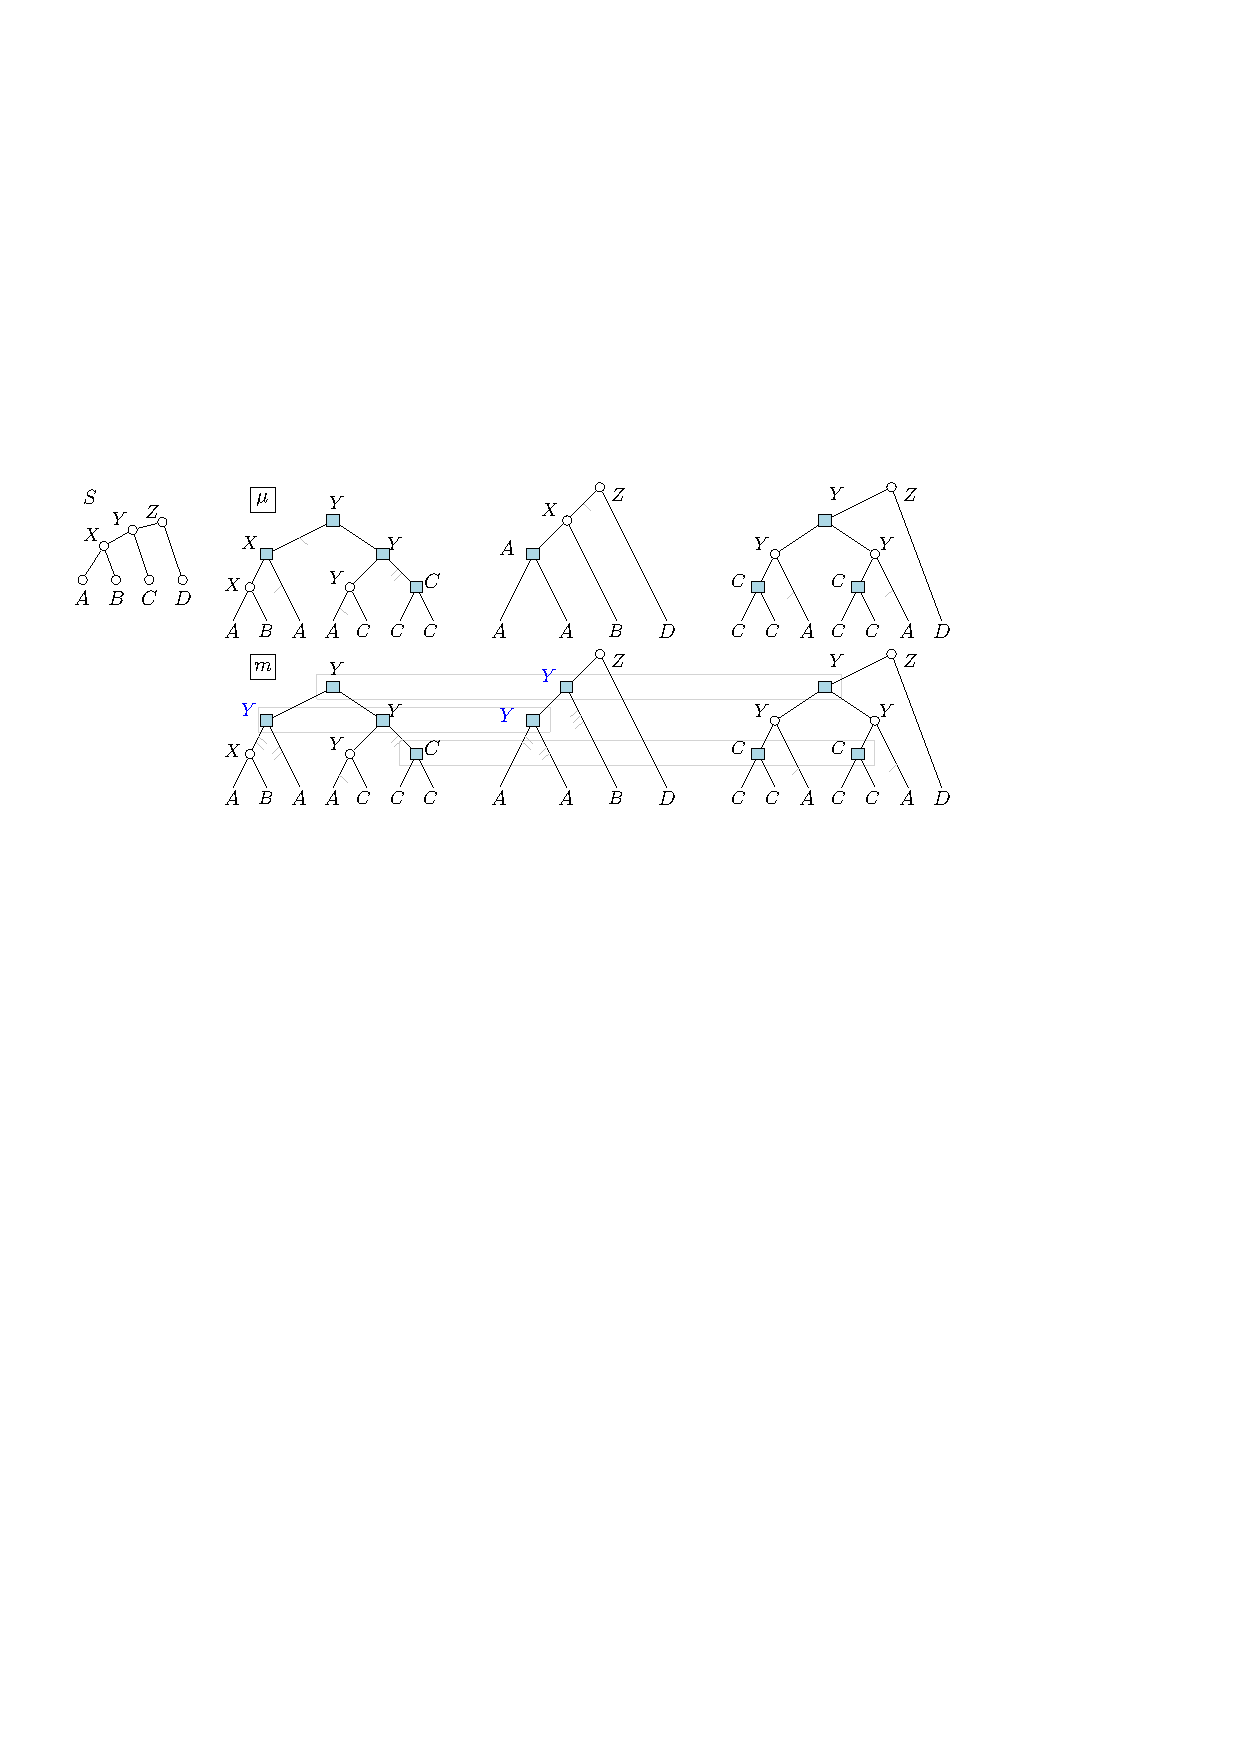
\includegraphics[width=0.8\linewidth]{figs_theory/fig1.pdf}
    \caption{Two possible segmental reconciliations for the same set of gene trees.  The top row shows a species tree $S$ with a gene forest of three gene trees.  The leaves are labeled by $\sigma$, that is, the species that contains them, and the internal node labels represent the lca-mapping $\mu$. 
    Duplications are shown as a blue square,  speciations as a white circle, and losses as light gray edges.
    On the bottom row, an alternate reconciliation $m$ with modified mappings in blue.  This can be explained with three segmental duplications, highlighted by gray rectangles.
    }
    \label{fig:fig1}
\end{figure}



Let $G$ be a gene forest, $S$ a species tree, $\sigma$ a leaf species map, and $m$ a reconciliation.  The \emph{event labeling under $m$} is a function $ev_m : V(G) \setminus L(G) \rightarrow \{Spec, Dup\}$ that assigns an event to each ancestral gene as follows.
Let $u$ be an internal node of $G$ and let $u_1$ and $u_2$ be its two children. 
Then:
% \begin{itemize}
%     \item if $m(u_1)$ and $m(u_2)$ are incomparable and $m(u)=lca(m(u_l),m(u_r))$, then $ev_m(u) = Spec$;
%     \item otherwise, $ev_m(u) = Dup$.
% \end{itemize}
\begin{align*}
    ev_m(u) = \begin{cases}
        Spec & \mbox{if $m(u_1)$ has children $x_1, x_2$ such that} \\
        & \mbox{$u_1 \preceq_S x_1$ and $u_2 \preceq_S x_2$}\\
        Dup &\mbox{otherwise.}
    \end{cases}
\end{align*}
A node $u \in V(G)$ with $m(u) = s$ and $ev_m(u) = Dup$ is called an \emph{$s$-duplication} (with respect to $m$).
In essence, $u$ is a speciation when its two child gene descend from the two distinct species that resulted from the speciation event.  Notice that such a node could be predicted as a duplication, but it was shown that under parsimony, if a node can be a $Spec$ according to $m$, then it should be a $Spec$.  As an example, in middle gene tree of Figure~\ref{fig:fig1}, the node mapped to $X$ according to $\mu$ is a $Spec$ (top), but the same node mapped to $Y$ according to $m$ is a $Dup$ (bottom).

Gene losses are counted on the branches of $G$ by listing the species that should be present but are not.  More specifically, for an edge $uv \in E(G)$, with $u$ the parent of $v$, the number of losses on $uv$ is 
\begin{align*}
    l_m(uv) = \begin{cases}
        dist_S(m(u), m(v)) - 1 &\mbox{if $ev_m(u) = Spec$} \\
        dist_S(m(u), m(v)) &\mbox{if $ev_m(u) = Dup$}
    \end{cases}
\end{align*}

% \begin{itemize}
%     \item if $m(u)$ is a speciation: number of loss for node $u$ is $l(u)=dist(m(u),m(u_l))+dist(m(u),m(u_r))-2$ where $dist$ returns the distance between two nodes (number of edges between two nodes).
%     \item if $m(u)$ is a duplication: number of loss for node $u$ is $l_m(u)=dist(m(u),m(u_l))+dist(m(u),m(u_r))$.
% \end{itemize}

The total number of losses under $m$ is
    $l_m = \sum_{uv \in E(G)} l_m(uv)$.
In the traditional DL model, the goal is to find a reconciliation that minimizes the number of $Dup$ nodes plus the number of losses.  We now turn to our segmental model.





\subsubsection*{Segmental duplications}




For a reconciliation $m$ and a species $s \in V(S)$, the \emph{duplication forest} of $s$ (under $m$), denoted $F_m(s)$ is the subgraph of $G$ induced by the duplications mapped to $s$:
\[
F_m(s) = G[ \{v \in V(G) : m(v) = s \mbox{ and } ev_m(v) = Dup\}].
\]
A segmental duplication is a single duplication event that contains multiple genes.  Since such genes must coexist, they must be incomparable in $F$, and it is not hard to see that 
the smallest possible number of segmental duplications in species $s$ is the height of $F_m(s)$.  As a shorthand, we write $H_m(s) = h(F_m(s))$ to denote that height.  The total number of segmental duplications according to $m$ is
\begin{align*}
    d_m = \sum_{s \in V(S)} H_m(s).
\end{align*}
For example in Figure~\ref{fig:fig1}, $d_{\mu} = 5$ (two duplications in $Y$, one in $X, A, C$), whereas $d_m = 3$ (two duplications in $Y$, one in $C$).


We can finally state our formulation.

\medskip

\noindent 
The \textsc{Most Parsimonious Segmental Reconciliation}

\noindent 
\textbf{Input:} a gene forest $G$, a species tree $S$, a leaf species map $\sigma$, and a duplication cost $\delta$ and loss cost $\lambda$.

\noindent 
\textbf{Goal:} find a reconciliation $m$ between $G$ and $S$ that minimizes
$\delta \cdot d_m + \lambda \cdot l_m$.
% \[\delta \cdot \left( \sum_{s \in V(S)} H_m(S) \right) + \lambda \cdot \left( \sum_{uv \in E(G)} l_m(uv) \right)\]

\medskip

We note that it was shown in [REF] that the lca-mapping $\mu$ is a solution for the problem when $\delta \leq \lambda$, but otherwise the problem is NP-hard.






\section{Efficient exploration of the solution space}

Since the \textsc{Most Parsimonious Segmental Reconciliation} is NP-hard, we turn to algorithms that can explore the space of solutions efficiently.  
We propose the following basic strategy:  

\medskip

\noindent
1) start with an initial reconciliation $m$ (typically $\mu$); \\
2) for each gene node $u \in V(G)$, and for each species $s$ that $u$ could possibly be mapped to, compute the change in cost in $m$ if we remap $u$ to $s$; \\
3) choose one of the remapping moves from the previous step according to some criteria, and apply the remapping; \\
4) repeat step 2 until no more moves need to be considered.

\medskip

In the following, we clarify what is meant by ``possibly mapped to'' and ``applying the remapping'', and later on discuss concrete strategies to choose moves and stop exploring. 
In what follows, we let $G$ be a gene forest, $S$ a species tree, and $m$ is a reconciliation on which we want to apply a move.  We consider the following types of moves.

\begin{figure}
    \centering
    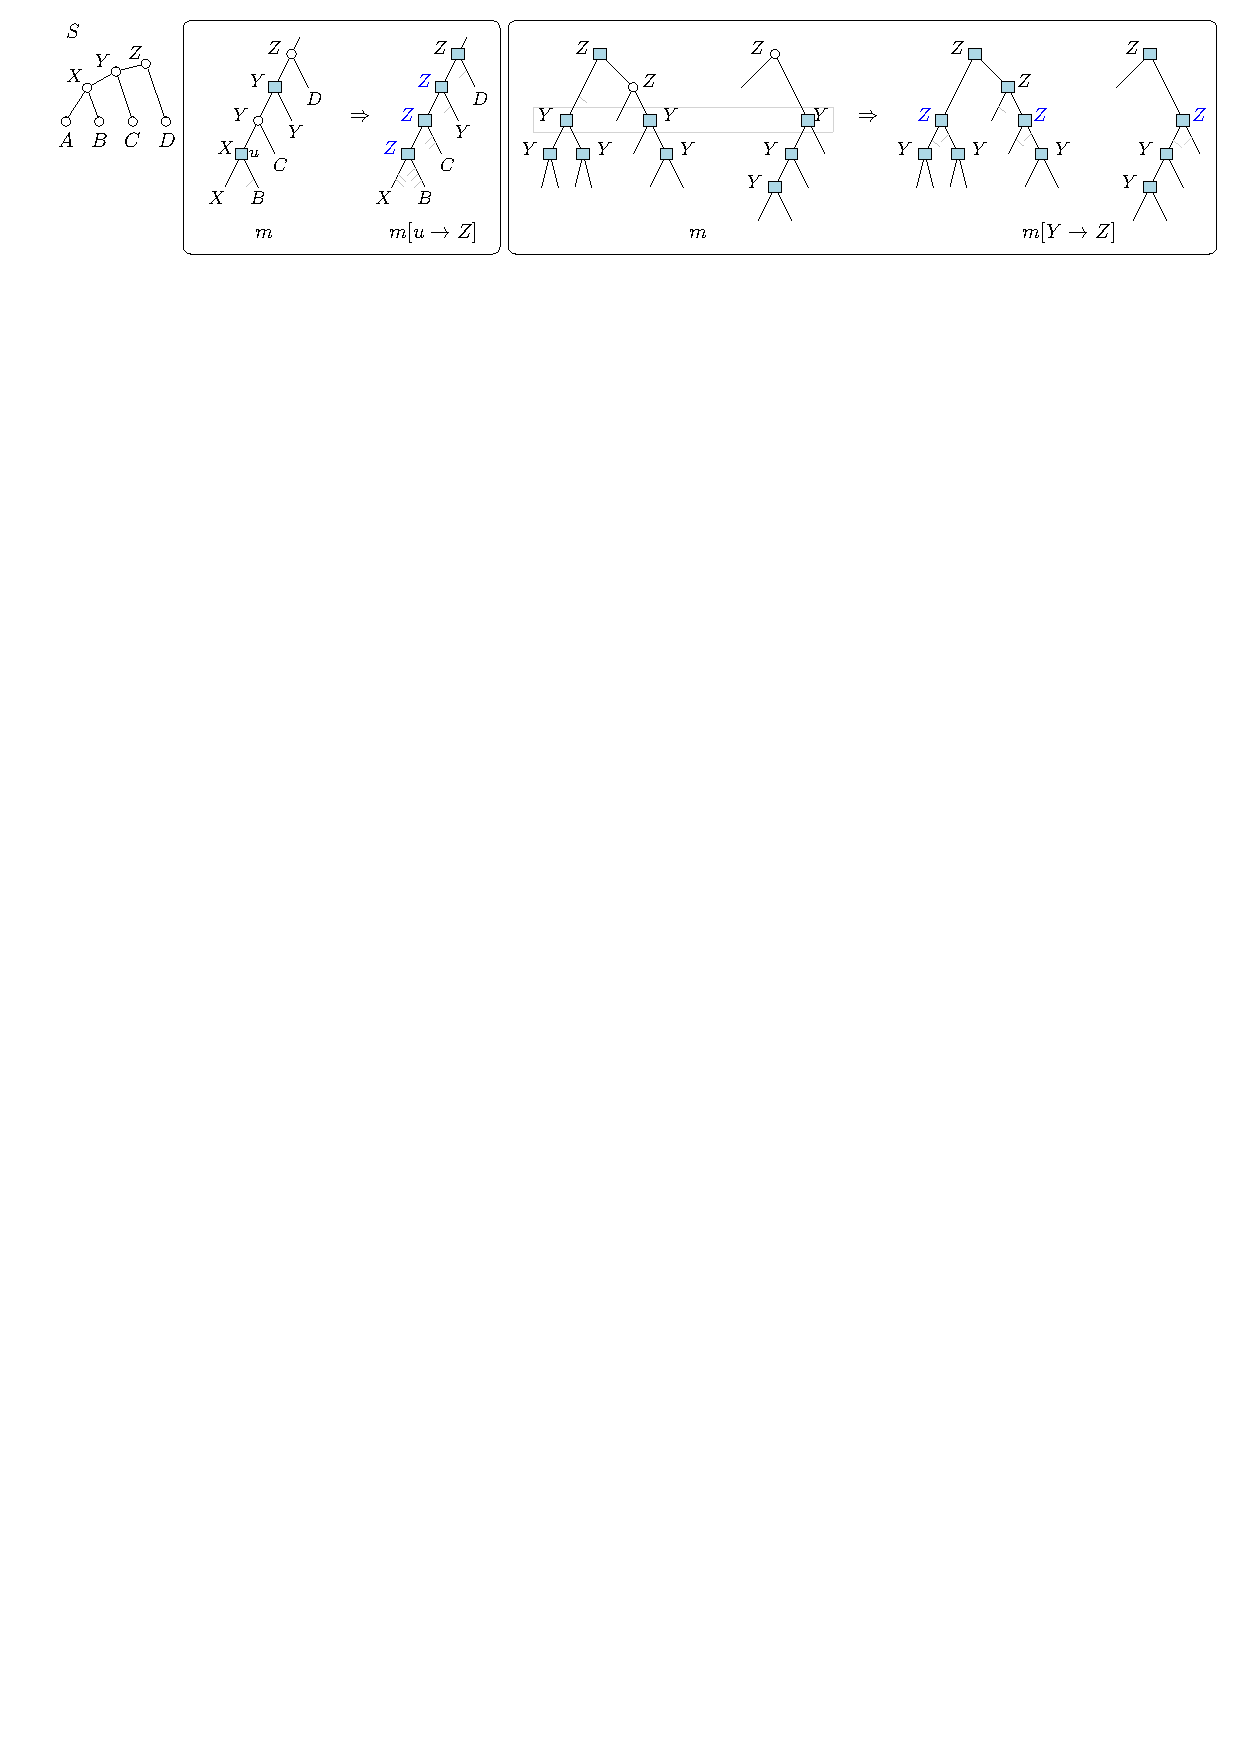
\includegraphics[width=1\linewidth]{figs_theory/upmoves.pdf}
    \caption{An illustration of up-moves and bulk up-moves.  Left: the species tree $S$.  Middle: a portion of a gene tree undergoing an up-move that remaps $u$ from $X$ to $Z$.  To satisfy time-consistency, the parent and grand-parent of $u$ must also be remapped to $Z$, which creates a chain of duplications in $Z$ and additional losses.  Right: a bulk up-move that takes the earliest segmental duplication in $Y$ spanning two gene trees, which consists of the roots of the trees in $F_m(Y)$, and remaps them to the species $Z$.}
    \label{fig:up-moves}
\end{figure}

\medskip 

\noindent 
\textbf{Up-moves.}
Let $u \in V(G)$ and let $s \succ m(u)$.
A node $u \in V(G)$ can be mapped to any ancestor of $\mu(u)$.  Such a remapping may create time inconsistencies, for instance if we remap $u$ to a species that pre-existed $m(p_u)$, where $p_u$ is the parent of $u$.  We therefore support remapping moves that can also remap ancestors to preserve time-consistency.  See Figure~\ref{fig:up-moves} left box for an example, where remapping $u$ to $Z$ enforces remapping all the ancestors in $Y$.

The \emph{up-remapping of $u$ to $s$} is another mapping denoted $m[u \rightarrow s]$ in which:
\begin{itemize}
    \item 
    $m[u \rightarrow s](w) = s$ for every ancestor $w$ of $u$ such that $m(w) \prec s$ (including $u$);

    \item 
    $m[u \rightarrow s](w) = m(w)$ for every other node of $G$.
    
\end{itemize}
The astute reader may ask whether up-moves that remap parents are necessary, as it would be simpler to only consider moves that do not remap the parent.  Let us call this a \emph{simple} up-move.  The middle gene tree in Figure~\ref{fig:fig1} shows the advantage of the more complex type of up-moves.  In that tree, we would like the $A$-duplication to be remapped to $Y$ to save one duplication, but with simple moves we would need to remap $X$ to $Y$ first.  However, that moves does not decrease the number of segmental duplications, but increases the number of losses, so it is strictly worse.  The more complex remap from $A$ to $Y$ lets us find an improved reconciliation directly, without having to go through a worse reconciliation first.


\medskip 

\noindent
\textbf{Bulk up-moves.}  We may need to remap several genes upwards to save a segmental duplication.  One way is to take the genes in the same segmental duplication in some species $s$, and move that duplication to an ancestor of $s$.
For $s \in V(S)$ and $t \succ s$, the \emph{bulk up-remapping from $s$ to $t$}
is another mapping $m[s \rightarrow t]$ in which, for every root $u$ of the forest $F_m(s)$ in any order, we apply the up-move that remaps $u$ to $t$.  



Note that such bulk up-moves always reduce the height of $F_m(s)$, although it can increase
the duplication height of other species.  
This is illustrated in Figure~\ref{fig:up-moves}, where the roots of the $Y$ duplication forest are all remapped to $Z$, thereby reducing the number of segmental duplications in $Y$.  Also note that such a move is guaranteed to increase the number of losses.  Therefore, they can only be advantageous if they reduce the height of $F_m(s)$ without increasing another height.  
%A bulk up-remapping from $s$ to $t$ will be called \emph{admissible} if $d_{m[s \rightarrow t]} < d_m$. 






\medskip 

\noindent 
\textbf{Down-moves.}
A down-move remaps $u \in V(G)$ to a species $s$ below $m(u)$.  Since $\mu(u)$ is the lowest possible, such an $s$ must satisfy $\mu(s) \preceq s \prec m(u)$, and we may need to remap descendants of $u$ to $s$ to avoid time-inconsistencies.
The \emph{down-remapping of $u$ to $s$} is another mapping $m[u \rightarrow s]$ in which
\begin{itemize}
    \item 
    $m[u \rightarrow s](w) = s$ for every descendant $w$ of $u$ such that $m(w) \succ s$ (including $u$);

    \item 
    $m[u \rightarrow s](w) = m(w)$ for every other node of $G$.
    
\end{itemize}


Notice that the notation $m[u \rightarrow s]$ does not distinguish between up-moves and down-moves, that distinction can be deduced from $s$.
Also note that unlike up-moves, applying a down-move to $u$ may make it change from a $Dup$ node to a $Spec$, and even its parent $p_u$ can become a $Spec$.


\medskip 

\noindent
\textbf{Bulk down-moves.} As for up-moves, several genes may be remapped ``downwards'' at once to save a duplication (or more).  Here, we take the deepest segmental duplication in $s$, and move it to a lower species.

For $s \in V(S)$ and $t \prec s$, the \emph{bulk remapping from $s$ to $t$} is another mapping $m[s \rightarrow t]$ that takes each deepest leaf $u$ of $F_m(s)$, that is, every $u$ of depth $H_m(s)$ in $F_m(s)$, and applies the down-remapping of $u$ to $t$.  If such a down-move is not possible because $\mu(u) \preceq t \prec s$ does not hold, then $m[s \rightarrow t]$ is \emph{invalid}.  
Note that valid bulk down-remappings always reduce the number of losses (see~\cite{dondi2019reconciling}), and hence they are advantageous if they do not increase the number of segmental duplications.  


\subsubsection*{Exploration strategies and bottlenecks}

We implemented standard \emph{greedy} and \emph{stochastic} strategies.
In the greedy strategy, we (1) start from the lca-mapping $\mu$; (2) compute the change in cost of every possible up, down, bulk-up, and bulk-down move; (3) apply the move that reduces the cost by a maximum amount, and repeat the second step.  We stop when, at step 3, every move strictly increases the reconciliation cost.

The stochastic strategy uses a simulated annealing algorithm by assigning a probability from the Boltzmann distribution to each move, based on its change in cost.  
The process is as follows:
\begin{enumerate}
    \item 
    start with $m = \mu$ as the lca-mapping;

    \item 
    for each possible move that results in a new reconciliation $m'$, compute $r = \delta (d_{m'} - d_m) + \lambda (l_{m'} - l_m)$, which is the change in reconciliation cost if we apply the move;

    \item 
    assign the weight $w_{m'} = e^{r / (kT)}$, where $k$ is the Boltzmann constant and $T$ is a user-specified \emph{temperature} parameters that specifies how likely the most cost-reducing moves are taken;

    \item 
    obtain a vector of weights $(w_{m_1}, \ldots, w_{m_l})$ from the list of computed moves.  Normalize the vector so that its entries sum to one, and use it as a probability distribution to sample an element from the vector, and apply the chosen move to obtain an updated reconciliation;

    \item 
    repeat Step 2 until convergence (i.e., no improvement in cost was made for a specified number of iterations), or until a specified maximum number of iterations is reached.
\end{enumerate}

The main bottleneck of this procedure is Step 2, the computation of cost changes of each move. 
In order to perform as many iterations as possible, our goal is to compute all such entries as efficiently as possible.  
However, a purely naive algorithm would be too slow.
Consider the set of all possible up-moves, for example.
Let us note that every node $u \in V(G)$ must be mapped to an ancestor $s$ of $\mu(u)$, and so there are $O(h(S))$ possibilities, and therefore $O(|V(G)|h(S))$ entries to compute. 
For each such entry, the naive algorithm would recalculate the forest heights in every gene tree in time $O(|V(G)| + |V(S)|)$ (which is actually difficult to avoid, because chains of remapping may affect several duplication heights).  
If we assume that $|V(G)| > |V(S)|$,  we get a total time of $O(|V(G)|^2 h(S))$ to compute every entry, per iteration.
 
Since our goal is to scale to gene forests with thousands of trees, and thus tens of thousands of nodes, a quadratic dependency on $|V(G)|$ is not acceptable to perform large numbers of iterations.  The complexity can be reduced by maintaining the forest heights per species in each gene tree separately, so that remappings only involve recalculations in the current tree, but the complexity per entry would still be linear in the size of that tree, plus the number of trees and $|V(S)|$.  In the following, we aim for an amortized time of $O(1)$ per entry.

\subsection{Computing the change in cost of up-moves}

We now describe in detail how the change in cost of each up-move can be computed efficiently.  
Consider a valid up-move $m[u \rightarrow s]$ that remaps $u$ to $s \succ m(u)$. 
For any $t \in V(S)$, 
we denote $\Delta(u, s, t) = H_{m[u \rightarrow s]}(t) - H_m(t)$, which is the change in duplication height in species $t$ after remapping $u$ to $s$. 
Note that $\Delta(u, m(u), t) = 0$, since remapping $u$ to $m(u)$ changes nothing.
Then denote
\[
\Delta(u, s) = \sum_{t \in V(S)} \Delta(u, s, t)
\]
which is actually equal to $d_{m[u \rightarrow s]} - d_m$, the \emph{total} change in duplication heights after remapping $u$ to $s$. 

We also need to account for losses, and denote by $\Lambda(u, s)$ the total change in the number of losses after remapping $u$ to $s$.  Recalling that $l_m$ is the number of losses in $m$, we have
\[
\Lambda(u, s) = l_{m[u \rightarrow s]} - l_m.
\]





\subsubsection{Changes in duplication costs}

Let us first focus on $\Delta(u, s)$ entries first.
We first show that if we calculate those in pre-order on $G$ (i.e, parents are handled before children), then we can re-use the information from the parents and only require a constant number of entries.  

\begin{toappendix}
In the following, we provide the complete formal arguments on the correctness of our up-moves computations.  
We first show that only the changes in $m(u)$ and $s$ need specific calculation, as $Dup$ nodes in other species are the same whether we remap $u$ to $s$ or its parent $p_u$ to $s$.

\begin{lemmarep}\label{lem:parent-remap-t}
    Let $u \in V(G)$ be a non-root vertex with parent $p_u$, let $s \in V(S)$ be an ancestor of $m(p_u)$, and let $t \in V(S) \setminus \{s, m(u)\}$.  
    Then $F_{m[u \rightarrow s]}(t) = F_{m[p_u \rightarrow s]}(t)$, that is, the set of $Dup$ nodes mapped to $t$ is the same under $m[u \rightarrow s]$ or $m[p_u \rightarrow s]$.
\end{lemmarep}

\begin{proof}
    Assume as stated that $s \succeq m(p_u)$, and observe that for a gene forest node $w \neq u$, $w$ is an ancestor of $u$ with $m(w) \prec s$ if and only if $w$ is an ancestor of $p_u$ with $m(w) \prec s$, because $u$ and $p_u$ have the same ancestors except $u$ itself.  Let $R_u$ (resp. $R_{p_u}$) be the ancestors of $u$ (resp. $p_u$) such that $m(w) \prec s$, noting that $R_{p_u} = R_u \setminus \{u\}$.
    Note that $R_u$ contains precisely the nodes that get remapped to $s$ in $m[u \rightarrow s]$ (the $R$ stands for ``remapped'').  Also note that $R_{p_u}$ could be empty if $s = m(p_u)$.
    
    Let $t \in V(S) \setminus \{s, m(u)\}$. 
    Let $w \in F_{m[u \rightarrow s]}(t)$, so that $w$ is a $Dup$ node under $m[u \rightarrow s]$ such that $m[u \rightarrow s](w) = t$.  Then $w \notin R_u$, since such ancestors get remapped to $s$ in $m[u \rightarrow s]$.  Hence $m(w) = m[u \rightarrow s](w) = t$. Also, $w \notin R_{p_u}$, so it does not get remapped in $m[p_u \rightarrow s]$ as well, and thus $m[p_u \rightarrow s](w) = t$.  
    We must also show that $w$ is a $Dup$ node under $m[p_u \rightarrow s]$.  To see this, consider the children $w_1, w_2$ of $w$ in $G$ (which exist since $Dup$ nodes are internal).  If no child of $w$ is in $R_u$, then no child of $w$ is in $R_{p_u}$, implying that $m[u \rightarrow s](w_i) = m[p_u \rightarrow s](w_i)$ for $i = 1,2$.  Since $Dup$ nodes are determined by the mapping of their children, we have that $w$ is a $Dup$ node under $m[p_u \rightarrow s]$ as well.
    It is also possible that one child $w_i$ of $w$ is in $R_u$ (but not two, since $R_u$ induces a path).  If that child is also in $R_{p_u}$, we have $s = m[u \rightarrow s](w_i) = m[p_u \rightarrow s](w_i)$.  The other child of $w$ is not in $R_u$ and does not change its map, and we get the same conclusion.  If that child $w_i$ is not in $R_{p_u}$ but is in $R_u$, then $w_i = u$ is the only possibility.  Hence $w_i = p_u$.  But this cannot be, because $p_u \notin R_{p_u}$ is only possible if $s = m(p_u)$, whereas we have $m(w) = t$.  Hence, we deduce that $w$ is a $Dup$ node mapped to $t$ if we remap $p_u$ to $s$, and thus $F_{m[u \rightarrow s]}(t) \subseteq F_{m[p_u \rightarrow s]}(t)$.
    
    Conversely, let $w \in F_{m[p_u \rightarrow s]}(t)$ be a $Dup$ node under $m[p_u \rightarrow s]$ such that $m[u \rightarrow s](w) = t$.  Similarly as before, $w \notin R_{p_u}$ and thus $m(w) = t$.  Moreover, $t \neq m(u)$  implies that $w \neq u$.  Therefore, $w \notin R_u$, and thus $m[u \rightarrow s](w) = m(w) = t$. 
    As before, consider the children $w_1, w_2$ of $w$.  If none of them is in $R_{p_u}$, then none of them is in $R_u$ (since $w \neq p_u$), and if one of them is in $R_{p_u}$, that child is also in $R_u$.  Thus the children of $w$ has the same map and it is also a $Dup$ node mapped to $t$ under $m[u \rightarrow s]$.  Hence $F_{m[p_u \rightarrow s]}(t) \subseteq F_{m[u \rightarrow s]}(t)$.
\end{proof}

Lemma~\ref{lem:parent-remap-t} allows us to simplify the computation of changes in cost.
\end{toappendix}

\begin{lemmarep}\label{lem:deltasum}
    Let $u \in V(G)$ and let $s \in V(S)$ be an ancestor of $m(u)$.
    If $u$ is a root, or if $u$ has parent $p_u$ satisfying $s \prec m(p_u)$, then
    \[
    \Delta(u, s) = \Delta(u, s, s) + \Delta(u, s, m(u)).
    \]
    Otherwise, $u$ has a parent $p_u$ satisfying $s \succeq m(p_u)$, in which case
    \begin{align*}
    \Delta(u, s) = \Delta(p_u, s) &~- \Delta(p_u, s, s) - \Delta(p_u, s, m(u)) \\
    &~+ \Delta(u, s, s) + \Delta(u, s, m(u)).
    \end{align*}
\end{lemmarep}

\begin{proofsketch}
	If $u$ is a root, it suffices to notice that only $u$ gets remapped, and only the heights in $m(u)$ and $s$ can change.    If $s \prec m(p_u)$, again only the $u$ gets remapped, and the type of $p_u$ ($Spec$ or $Dup$) does not get affected, and the same argument applies.  In the last case, the remapping only affects duplications in $s, m(u)$, or $t$ with $m(u) \prec t \prec s$.  For those, the set of $t$-duplications that get removed is the same whether we remap $u$ to $s$ or $p_u$ to $s$, because such a duplication must be a strict ancestor of $u$.  Hence the difference in duplication heights for those $t$'s is already counted in $\Delta(p_u, s)$.  It is possible to have differences in $s$ or $m(u)$ though, so we take $\Delta(p_u, s)$, remove $\Delta(p_u, s, s)$ and $\Delta(p_u, s, m(u))$ which could be different, and replace them with $\Delta(u, s, s)$ and $\Delta(u, s, m(u))$.
\end{proofsketch}

\begin{proof}
    Suppose that $u$ is a root of $G$.  Since up-moves can only remap ancestors of $u$, it follows that $u$ is the only node that gets remapped in $m[u \rightarrow s]$.  Hence, aside from $u$, all the nodes have the same map as well as their children, and therefore $Dup$ nodes mapped to $t \notin \{m(u), s\}$ are the same in either $m$ or $m[u \rightarrow s]$, and thus $\Delta(u, s, t) = 0$ for each such $t$.  Therefore, the summation for $\Delta(u, s)$ can only be affected by $\Delta(u, s, s)$ and $\Delta(u, s, m(u))$, as stated.
    
    If $u$ is not a root but $s \prec m(p_u)$, it is still true that all nodes except $u$ keep the same map under $m[u \rightarrow s]$, including $p_u$. 
    Moreover, the children of all such nodes have the same map, except $p_u$ whose child $u$ has changed.
    Thus all $Dup$ nodes in $t \neq s, m(u)$ are the same before and after, except possibly $p_u$.
    If $p_u$ is a $Dup$ under $m$, it is easy to check that this also holds under $m[u \rightarrow s]$.  If $p_u$ was a $Spec$, then $m(p_u)$ has children $x_1, x_2$ and $m(u) \preceq x_1$ (and the other child descends from $x_2$).  Since $m(u) \preceq s \prec m(p_u)$, we have $s \preceq x_1$ as well and $p_u$ is still a $Spec$ under $m[u \rightarrow s]$.  Hence, duplication forests in $t$ are also preserved in this case.  It again follows that only $\Delta(u, s, s)$ and $\Delta(u, s, m(u))$ contribute to $\Delta(u, s)$. 
    

    So assume that $s \succeq m(p_u)$.
    By Lemma~\ref{lem:parent-remap-t}, 
    for $t \notin \{m(u), s\}$, the $Dup$ nodes in $t$ are identical under $m[u \rightarrow s]$ and $m[p_u \rightarrow s]$.  
    It follows that $H_{m[u \rightarrow s]}(t) = H_{m[p_u \rightarrow s]}(t)$, and therefore that $\Delta(u, s, t) = \Delta(p_u, s, t)$.
    We may conclude that 
    \begin{align*}
        \Delta(u, s) &= \sum_{t \in V(S)} \Delta(u, s, t) \\
        &= \Delta(u, s, s) + \Delta(u, s, m(u)) + \sum_{t \in V(S) \setminus \{s, m(u)\}} \Delta(u, s, t) \\
        &= \Delta(u, s, s) + \Delta(u, s, m(u)) + \sum_{t \in V(S) \setminus \{s, m(u)\}} \Delta(p_u, s, t) \\
        &= \Delta(u, s, s) + \Delta(u, s, m(u)) + \Delta(p_u, s) - \Delta(p_u, s, s) - \Delta(p_u, s, m(u))
    \end{align*}
    which, after reordering the terms, yields the claimed equality.
\end{proof}



    As a consequence of Lemma~\ref{lem:deltasum}, using a top-down approach, one can obtain $\Delta(u, s)$ by reusing $\Delta(p_u, s)$ and computing only four additional values, at most.
    Still, these are not trivial to obtain in $O(1)$ time, and we need auxiliary data structures to achieve this efficiently\footnote{\ml{Illustrate those concepts.  Also I am boring myself at this point, too much notation to remember, any way to reduce the dryness of the text?}}.  Later on we discuss how to maintain this information while still achieving $O(1)$ time per entry.

\begin{itemize}
    
    \item 
    For a $Dup$ node $u \in V(G)$ under $m$, denote by $h_m(u)$ the height of $v$ in $F_m( m(u) )$.  
    That is, $h_m(u)$ is the number of segmental $m(u)$-duplications that contain $v$ or one of its descendants.

    
    \item 
    For $s \in V(S)$ and integer $k$, denote by $B[s, k]$ the set of nodes of $G$ whose height is $k$ in $F_m(s)$.  
    That is, $B[s, k] = \{v \in V(G) : m(v) = s, h_m(v) = k\}$. 

    \item 
    For $u \in V(G)$ and $s \succeq m(u)$, define $c_m(u, s)$ as the number of ancestors $v$ of $u$ satisfying $s \succeq m(v)$.
    %
    % \begin{align*}
    %     c_m(u, s) = \begin{cases}
    %         1 &\mbox{if $u$ is a root of $G$ or $s \prec m(p_u)$} \\
    %         c_m(p_u, s) + 1 &\mbox{otherwise}
    %     \end{cases}
    % \end{align*}
    This quantity is the length of the duplication chain that ends at $u$ if we remap it to $s$.  
    
    
 
    % \item 
    % For $s \in V(S)$ and integer $k$, denote by $D[s, k]$ the set of nodes of $G$ whose depth is $k$ in $F_m(s)$.  
    % That is, $D[s, k] = \{v \in V(G) : m(v) = s, d_m(v) = k\}$.  

\end{itemize}



    
% \begin{figure}
%     \centering
%     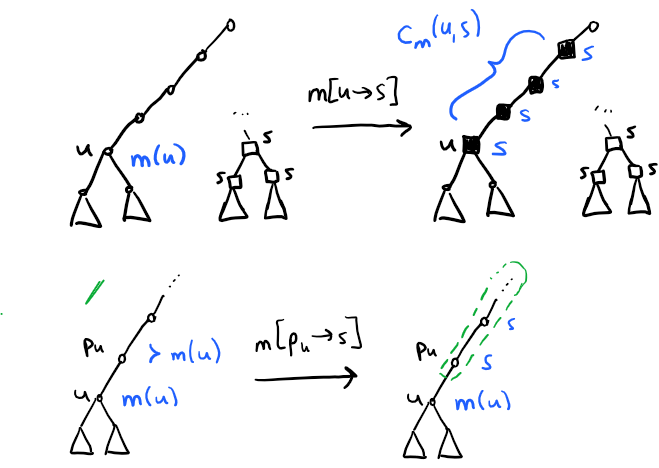
\includegraphics[width=0.7\textwidth]{deltauss.png}
%     \caption{Illustration of the cases covered by Lemma~\ref{lem:deltauss}.  Top shows $\Delta(u, s, s)$: the new height in $s$ in $m[u \rightarrow s]$ is either the chain in $s$ that ends at $u$, or the height of a subtree that was already there.
%     Bottom is $\Delta(p_u, s, m(u))$: if $m(p_u) \succ m(u)$, then in $m[p_u \rightarrow s]$ only ancestors of $p_u$ are affected, which does not change the height in $m(u)$.  Otherwise, $m(p_u) = m(u)$, as stated in Lemma~\ref{lem:deltauss}.}
%     \label{fig:deltauss}
% \end{figure}


\begin{figure}
    \centering
    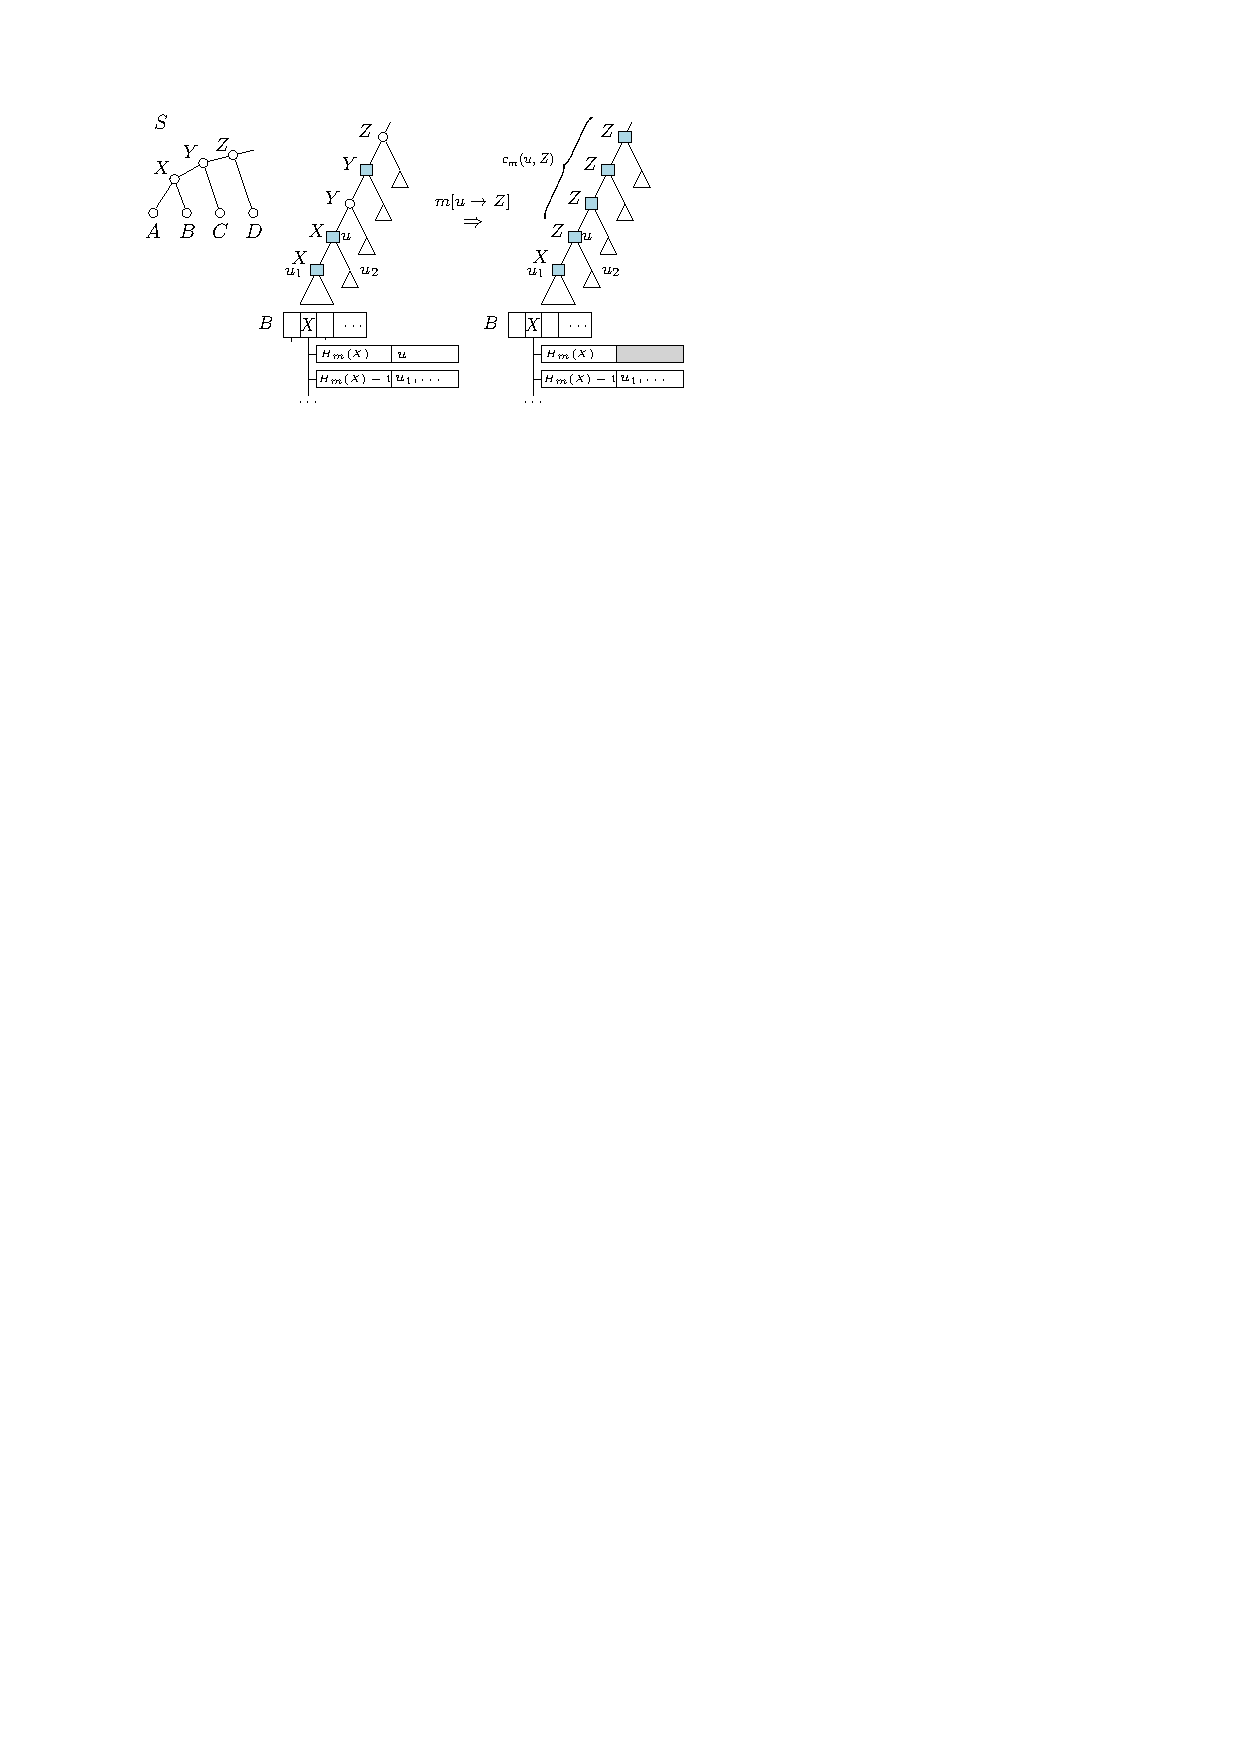
\includegraphics[width=0.65\linewidth]{figs_theory/cmu.pdf}
    \caption{Illustration of Cases 1 and 3.(a) from Lemma~\ref{lem:deltauss}. 
    For Case 1, $\Delta(u, s, s) = \Delta(u, Z, Z)$, and the length of the chain of $Z$-duplications ending at $u$ after remapping is $c_m(u, Z) = 4$.  Either this chain is the maximum height in $Z$-duplications after remapping, or some other untouched subtree still has the maximum height.  For Case 3.(a), $\Delta(u, s, m(u)) = \Delta(u, Z, X)$, a representation of $B$ is shown at the bottom.  If $B[s, H_m(s)] = B[X, H_m(X)]$ only contains $u$, then after remapping $u$ that entry becomes empty and a child $u_1$ of $u$ is now a root of a highest $X$-duplication subtree (of height $H_m(X) - 1$).}
    \label{fig:deltacases}
\end{figure}





Assuming we compute $\Delta(u, s, t)$ values in pre-order, the value of $\Delta(p_u, s, s)$ needed in Lemma~\ref{lem:deltasum} is easy to obtain: if $m(p_u) = s$, then it is $0$, and otherwise that value is necessary to compute $\Delta(p_u, s)$, and so it will have been computed and stored when handling $p_u$.  The next lemma states how the other three required values can be calculated.

\begin{lemmarep}\label{lem:deltauss}
    Let $u \in V(G)$ and let $s \in V(S)$ be a strict ancestor of $m(u)$.  Then the following holds:
    \begin{enumerate}
    \item 
    $\Delta(u, s, s) = \max(c_m(u, s) - H_m(s), 0)$.
    

    \item 
    If $u$ has a parent $p_u$ satisfying $s \succeq m(p_u)$, then 
    \begin{align*}
        \Delta(p_u, s, m(u)) = \begin{cases}
            0 &\mbox{ if $m(u) \prec m(p_u)$} \\
            \Delta(p_u, s, m(p_u)) &\mbox{ otherwise.} \\
        \end{cases}   
    \end{align*}

    
        \item 
        for the value of $\Delta(u, s, m(u))$, the following cases arise:

        \begin{enumerate}
            \item 
        if $u$ is a root or $m(u) \neq m(p_u)$, then
        \begin{align*}
            \Delta(u, s, m(u)) = \begin{cases}
                -1 &\mbox{if  $B[m(u), H_m(m(u))] = \{u\}$} \\
                0 &\mbox{ otherwise} 
            \end{cases}
        \end{align*}


        \item 
        if $m(u) = m(p_u)$, then let $h' = H_{m[p_u \rightarrow s]}(m(u)) = H_m(m(u)) + \Delta(p_u, s, m(u))$, which is the height in $m(u)$ if we remap $p_u$ to $s$.  
        Then
        \begin{align*}
            \Delta(u, s, m(u)) = \Delta(p_u, s, m(u)) + \begin{cases}
                0 &\mbox{ if $h' \neq h_m(u)$} \\
                -1 &\mbox{ if $h' = h_m(u)$ and $B[m(u), h'] = \{u\}$} \\
                0 &\mbox{ if $h' = h_m(u)$ and $B[m(u), h'] \neq \{u\}$} 
            \end{cases}
        \end{align*}
    \end{enumerate}
    


    
\end{enumerate}
\end{lemmarep}


\begin{proofsketch}
For 1., one can show that the longest $s$-duplication path in $m[u \rightarrow s]$ either starts at $u$ and goes upwards, in which case the length of the path is $c_m(u, s)$, or the longest $s$-duplication path was already present and there is $0$ change.  
For 2., if $m(u) \prec m(p_u)$, then remapping $p$ to $s$ does not affect any node mapped to $m(u)$, and otherwise only $m(u) = m(p_u)$ is possible.  
For 3.(a), the height in $m(u)$ cannot increase, and the only way to decrease it is if $u$ was the sole root of a maximum-height tree in $F_m(m(u))$.
This holds if and only if $B[m(u), H_m(m(u))] = \{u\}$, and the height can only drop by $1$ since the children of $u$ keep the same map.

For 3.(b), we rely on $h'$, the height in $m(u)$ if we remap $p_u$ to $s$.  In $m[p_u \rightarrow s]$, one of three things can happen: $u$ is not the root of a maximum height subtree in $m(u)$ (in which case $h' \neq h_m(u)$ and $\Delta(u, s, m(u)) = \Delta(p_u, s, m(u))$); $u$ is the sole root of a maximum height subtree, in which case $h' = h_m(u)$ and $B[m(u), h'] = \{u\}$ and now remapping $u$ decreases the duplication height; or there are multiple roots of maximum height subtrees, in which case there is no change in heights.  The expression for $\Delta(u, s, m(u))$ considers these three cases.
\end{proofsketch}


\begin{proof}
    We argue the three values separately.

    \noindent
    \textbf{Case 1: $\Delta(u, s, s)$.}
    Consider $\Delta(u, s, s)$ first.  
    First note that under $m[u \rightarrow s]$, is a $Dup$ node in $s$ and none of its children is mapped to $s$.  
    Consider the path $P$ that starts at $u$ and, going upwards, includes the ancestors of $u$ mapped to $s$ in $m[u \rightarrow s]$.
    Then $P$ includes $u$, plus any ancestor $v$ of $u$ that got remapped (so $s \succ m(v)$), plus any ancestor $v$ such that $s = m(v) = m[u \rightarrow s](v)$.  Thus by definition, the number of nodes of $P$ is equal to $c_m(u, s)$.

    We note that $H_{m[u \rightarrow s]}(s) \geq H_m(s)$, because the $m[u \rightarrow s]$ has strictly more $Dup$ nodes mapped to $s$ than $m$, namely because of $u$.  
    Now let $Q$ be a root-to-leaf path of maximum length in $F_{m[u \rightarrow s]}(s)$, so that the number of nodes in $Q$ is $H_{m[u \rightarrow s]}(s)$.  
    If $Q$ contains $u$, then $P = Q$ and 
    $\Delta(u, s, s) = c_m(u, s) - H_m(s)$.  Since this is at least $0$, our $\max$ expression is correct in this case.
   
    If $Q$ does not contain $u$, then $c_m(u, s) \leq H_{m[u \rightarrow s]}(s)$.  We also note that $Q$ could not contain an ancestor $v$ of $u$ such that $s \succ m(v)$.  Indeed, such a node $v$ has children not mapped to $s$ under $m$, and under $m[u \rightarrow s]$ it only has a child mapped to $s$ that leads to $u$.  Thus any maximal $Dup$ path in $s$ containing such a $v$ ends in $u$.
    Thus, $Q$ does not contain any node that got remapped from $m$ to $m[u \rightarrow s]$, and so that $Dup$ path in $s$ was also present under $m$.
    We thus get $H_{m[u \rightarrow s]}(s) \leq H_m(s)$, and because the duplication height in $s$ cannot decrease, equality holds and $\Delta(u, s, s) = 0$.  In that case, $c_m(u, s) \leq H_{m[u \rightarrow s]}(s)$ implies that our $\max$ expression will return $0$.  In all cases $\Delta(u, s, s)$ is correct.
    
 
 % The intuition is that the highest duplication subtree at $s$ is either a subtree that was already there, or is obtained from the chain of $s$ that ends at $u$.

    \medskip

    \noindent
    \textbf{Case 2: $\Delta(u, s, m(u))$.}
    For $\Delta(p_u, s, m(u))$, if $m(u) \prec m(p_u)$, then notice that no ancestor of $p_u$ is mapped to $m(u)$.  Therefore, remapping $p_u$ to $s$, which is an ancestor of $m(p_u)$ and thus of $m(u)$, cannot affect the duplication height in $m(u)$.  In this case, $\Delta(p_u, s, m(u)) = 0$ as stated.
    If instead $m(u) \succeq m(p_u)$, then by time-consistency, only $m(u) = m(p_u)$ is possible, hence $\Delta(p_u, s, m(u)) = \Delta(p_u, s, m(p_u))$.

    \medskip 

    \noindent 
    \textbf{Case 3: $\Delta(u, s, m(u))$.}
    We note that the height of the duplication forest in $m(u)$ cannot increase when remapping $u$ to $s$, since this remapping reduces the number of nodes mapped to $m(u)$.
    Suppose that $u$ is a root or $m(u) \neq m(p_u)$.  
    Suppose that $B[m(u), H_m(m(u))] = \{u\}$.  Then there is only one subtree of $F_m(m(u))$ of height $H_m(m(u))$ and its root is $u$.
    When we remap $u$ to $s$, the largest possible height in $m(u)$ is then $H_m(m(u)) - 1$, which is achieved by one of the children of $u$.  In this case, the duplication height in $m(u)$ is reduced by $1$, and so putting $\Delta(u, s, m(u)) = -1$ in this case is correct.
    So assume that $B[m(u), H_m(m(u))]$ contains some node $v$ other than $u$ (note that the $B$ entry cannot be empty).  Then $m(u) \neq m(p_u)$ implies that $v$ is not $p_u$ nor any of its ancestors.  Thus $v$ is incomparable with $u$, and thus the duplication subtree rooted at $v$ is still present in $m[u \rightarrow s]$.  Hence the height has not reduced, and since it cannot decrease, $\Delta(u, s, m(u)) = 0$ is the correct value to apply in this case.
    


    Next suppose that $m(u) = m(p_u)$.  Let $h' = H_{m[p_u \rightarrow s]}(m(u))$ be the height of the duplication forest in $m(u)$ under $m[p_u \rightarrow s]$. If $h' \neq h_m(u)$, then some subtree of height $h'$ in $m(u)$ is present under $m[p_u \rightarrow s]$ and is not rooted at any ancestor of $p_u$  (because those are mapped to $s$ or above).  It is also not rooted at $u$ since $h' \neq h_m(u) = h_{m[p_u \rightarrow s]}$.  It is therefore not rooted at an ancestor of $u$ and so this subtree is also present under $m[u \rightarrow s]$.  It follows that $H_{m[u \rightarrow s]}(m(u)) \geq h'$.  On the other hand, $H_{m[u \rightarrow s]}(m(u)) \leq  h'$, since $m[u \rightarrow s]$ has strictly less nodes mapped to $m(u)$ than $m[p_u \rightarrow s]$.  Thus $H_{m[u \rightarrow s]}(m(u)) = h'$, and we get 
    \[
    H_{m[u \rightarrow s]}(m(u)) - H_m(m(u)) = h' - H_m(m(u)) = \Delta(p_u, s, m(u))
    \]
    which is the correct value we give to $\Delta(u, s, m(u))$.
    
    
    So assume that $h' = h_m(u)$.  
    Then under $m[p_u \rightarrow s]$, $u$ is the root of a $Dup$ tree in $m(u)$ of maximum height.  If $B[m(u), h'] = \{u\}$, then $u$ is the only subtree with height $h'$ under $m$.  Noting that remapping $p_u$ and some ancestors to $s$ cannot create new $Dup$ subtrees in $m(u)$ with that same height, it follows that $u$ is also the only subtree with that height under $m[p_u \rightarrow s]$ as well.  Since the only difference between $m[u \rightarrow s]$ and $m[p_u \rightarrow s]$ is that $u$ is remapped to $s$, the height of that subtree is one less under $m[u \rightarrow s]$ than under $m[p_u \rightarrow s]$ (achieved by one of the children of $u$, as before).
    Thus putting $\Delta(u, s, m(u)) = \Delta(p_u, s, m(u)) - 1$ is correct in this case.

    Finally, suppose that $B[m(u), h']$ contains some node $v$ other than $u$.
    Because under $m$, $u$ and $v$ both root a $Dup$ subtree in $m(u)$ of the same height $h'$, $v$ cannot be an ancestor or descendant of $u$ and is thus incomparable with $u$.  Hence, the $v$ subtree is present under either $m[p_u \rightarrow s]$ or $m[u \rightarrow s]$. 
    Thus, $H_{m[u \rightarrow s]}(m(u)) \geq h'$ and, using the previous argument, $H_{m[u \rightarrow s]}(m(u)) \leq h'$.  This implies equality and then $\Delta(u, s, m(u)) = \Delta(p_u, s, m(u))$.
\end{proof}






\subsubsection{Changes in loss costs}

\ml{[ML if we run out of space, maybe send this to an appendix to give priority to experiment results.]}
Recall that $\Lambda(u, s) = l_{m[u \rightarrow s]} - l_m$ is the total change in the number of losses after remapping $u$ to $s$. 
For a mapping $m'$, we define:
        \begin{align*}
            i_{m'}(u) = \begin{cases}
                0 &\mbox{if  $u$ is duplication under $m'$} \\
                2 &\mbox{if  $u$ is speciation under $m'$}
            \end{cases}
        \end{align*}
Assuming that $s$ is a strict ancestor of $m(u)$, we also define an auxiliary value  $\lambda(u,s)$ as the total change in the number of losses between $u$ and its children $u_l, u_r$, that is:
    \begin{align*}
    \lambda(u, s) =~&dist(s , m(u_l))  - dist(m(u), m(u_l))~+ \\
    &dist(s , m(u_r)) -  dist(m(u), m(u_r)) + i_m(u)
    \end{align*}
The reason for adding the $i_m(u)$ term is that if $u$ is a $Spec$ under $m$, it will be a $Dup$ under $m[u \rightarrow s]$ and require additional loss on each child branch.

\begin{lemma}\label{lem:firstcaseloss}
    Let $u \in V(G)$ and let $s \in V(S)$ be a strict ancestor of $m(u)$.
    Then:

    \begin{enumerate}
        \item 
        If $u$ is a root, then $\Lambda(u, s) = \lambda(u, s)$.

        \item 
        if $u$ has a parent $p_u$ and $s \preceq m(p_u)$, then
        \begin{align*}
        \Lambda(u, s) = \lambda(u, s) +  ~&dist(m(p_u) , s) - dist(m(p_u), m(u))~+\\
        &i_{m}(p_u) - i_{m[u \rightarrow s]}(p_u).
        \end{align*}

        \item 
        if $u$ has a parent $p_u$ and $s \succ m(p_u)$, then
        \begin{align*}
        \Lambda(u, s) = \Lambda(p_u, s) + \lambda(u, s) - dist(s, m(u))
        \end{align*}
    \end{enumerate}
\end{lemma}

\begin{proof}
    If $u$ is a root, the only edges of $G$ on which the number of losses changes are those adjacent to $u$, which are the edges leading to the children of $u$.  In that case, the expression $\lambda(u, s)$ is easily seen to represent the number of changes in losses.
    
    Suppose that $u$ is not a root but $s \preceq m(p_u)$.  Then $p_u$ does not get remapped, and so the changes in number of losses only occur on the edges incident to $u$.  This includes the edges leading to the children of $u$, which again are handled by $\Lambda(u, s)$, but also the edge $(p_u, u)$.  
    If $p_u$ is a $Dup$ under $m$, then it must be a $Dup$ under $m[u \rightarrow s]$ as well since $s \succ m(u)$.
    In that case, the number of losses on $(p_u, u)$ under $m$ is $dist(m(p_u), m(u))$ and under $m[u \rightarrow s]$ it is $dist(m(p_u), s)$.  Since $i_m(p_u) = i_{m[u \rightarrow s]}$ in this case, our value of $\Lambda(u, s)$ is correct in this case. 

    If $p_u$ is a $Spec$ under $m$, it could be a $Spec$ or a $Dup$ under $m[u \rightarrow s]$.
    Suppose it remains a $Spec$.  
    Then the difference in the number of losses is 
    \[
    dist(m(p_u), s) - 1 - (dist(m(p_u), m(u) - 1))
    \]
    and our value of $\Lambda(u, s)$ is again correct.
    If $p_u$ becomes a $Dup$.  Let $v$ be the child of $p_u$ other than $u$.  Note the change from $Spec$ to $Dup$ adds an extra loss on $(p_u, v)$. 
    Then the difference in the number of losses is 
    \[
    dist(m(p_u), s) + 1 - (dist(m(p_u), m(u) - 1))
    \] 
    and, since $i_m(p_u) - i_{m[u \rightarrow s]}(p_u) = 2$, our value is correct.

    Finally, assume that $s \succ m(p_u)$. In this case, $p_u$ and some of its ancestors gets remapped.  In this case, one can see this remapping $u$ to $s$ in two phases: first remap $p_u$ to $s$, which introduces $\Lambda(p_u, s)$ losses, then remap $u$ to $s$.  Note that no losses remain on the $(p_u, s)$ edge after the second phase, so the losses on that edge counted in the first phase need to be subtracted.  Because $p_u$ is a $Dup$ after remapping it to $s$, there are $dist(s, m(u))$ losses on $(p_u, s)$ to subtract.  The only other change introduced by this second phase are the $\lambda(u, s)$ losses created on the children of $u$.  
    This justifies our expression for $\Lambda(u, s)$.
\end{proof}









\subsubsection{Wrapping up: complexity of computing every entry}

We have gathered all the necessary steps to compute $\Delta(u, s)$ for every $u \in V(G)$ and $s \succ m(u)$.  To achieve amortized $O(1)$ time per entry, we must argue that the set of all entries can be computed in total time $O(|V(G)|h(S))$.
Recall that we need access to values $h_m(u), B[s, k]$, $c_m(u, s)$, and $H_m(s)$.  We first assume that we have computed and stored the lca-mapping, that we may query in time $O(1)$ whether a node is an ancestor of the other, and that we have access to $dist_S(x, y)$ in $O(1)$ time (this pre-processing is only needed once before the first iteration and can be achieved in time $O(|V(G)| + |V(S)|)$).
To compute the necessary values:

\begin{enumerate}
    
    \item 
    the values $h_m(u)$ can be calculated in time $O(|V(G)|)$ through a post-order traversal of $G$.  If $u$ is a speciation, then $h_m(u) = 0$ because it is not even part of $F_m(m(u))$.  If $u$ is a duplication, then $h_m(u) = 1 + \max_{v \in C(u)} h_m(v)$, where $C(u)$ is the set of children of $u$ mapped to $m(u)$ (the maximum is defined as $0$ if $C(u)$ is empty).  Note that checking whether $u$ is a $Spec$ or $Dup$ can be done in $O(1)$ time by comparing $m$ with $\mu$.

    
    \item 
    for the the sets $B[s, k]$, assuming $O(1)$ time for searching and inserting into hash tables,$B$ can be filled in time $O(|V(G)|)$ by adding each $u$ to $B[s, h_m(u)]$.

    \item 
    the values $H_m(s)$ can easily be obtained while computing the previous step, as $H_m(s)$ is the maximum $k$ such that $B[s, k]$ is non-empty.

    \item 
    for the values $c_m(u, s)$, we compute them in time $O(|V(G)| h(S))$ through a pre-order traversal of $G$, where for each $u \in V(G)$ we iterate over every $s \succeq \mu(u)$, noting that constant time per $c_m$ entry can be done using the fact that $c_m(u, s) =
    1$ if $u$ is a root of $G$ or $s \prec m(p_u)$, and otherwise $c_m(p_u, s) + 1$.
\end{enumerate}

Overall, the pre-processing step takes time no more than $O(|V(G)|h(S))$.
Once this is done, we can compute $\Delta(u, s)$ and $\Lambda(u, s)$ for each $u$ and each $s$ in pre-order.  
By computing those in pre-order, one can check that the expressions from Lemma~\ref{lem:deltasum} and Lemma~\ref{lem:deltauss} can all be computed in time $O(1)$, if we have access to the entries of $p_u$ when arriving at a node $u$.  We thus get the following.
% \begin{itemize}
%     \item 
%     If $u$ is a root, then compute and store $\Delta(u, s, s)$ and $\Delta(u, s, m(u))$, and obtain $\Delta(u, s)$.
    
%     One can check from Lemma~\ref{lem:deltauss} that these values only require access to $c_m(u, s), H_m(s)$, and checkign whether $B[m(u), H_m(m(u))] = \{u\}$, which can all be done in constant time.
    
%     \item 
%     If $u$ is not a root, then compute and store $\Delta(u, s, s), \Delta(u, s, m(u)), \Delta(p_u, s, m(u)),$ and $\Delta(p_u, s, s)$, then obtain $\Delta(u, s)$.  
%     For the first three, one can check from Lemma~\ref{lem:deltauss} that they can all be computed in constant time using the pre-processed data structures and stored entries for $p_u$.  In particular, $\Delta(p_u, s, m(p_u))$ must have been computed when $s \succeq m(p_u)$, as well as $\Delta(p_u, s, m(u))$ when $m(u) = m(p_u)$.  
%     As for $\Delta(p_u, s, s)$, it is $0$ when $m(p_u) = s$, and otherwise, whether $p_u$ is a root or not, the value of $\Delta(p_u, s, s)$ had to be computed when handling $\Delta(p_u, s)$.

%     \item 
%     For losses, we assume that $dist(x, y)$ can be accessed in constant time for any pair of species nodes $x$ and $y$.  This can easily be achieved using a $O(|V(S)|)$ time pre-processing of $S$.
%     Thus each $\lambda(u, s)$ can be calculated in constant time, and since the expressions from Lemma~\ref{lem:firstcaseloss} only rely on $\lambda(u, s)$, species tree distances, and $\Lambda(p_u, s)$, each entry takes constant time.
    
% \end{itemize}

% Since the pre-processing time is $O(|V(G)|h(S))$ and each $\Delta(u, s)$ and $\Lambda(u, s)$ entry takes constant time, we get the following.

\begin{theorem}
Given a gene forest $G$, a species tree $S$, and a reconciliation $m$, the value of each possible entry for up-moves $\Delta(u, s)$ and $\Lambda(u, s)$ can be computed in total time $O(|V(G)|h(S))$.
\end{theorem}


\textbf{Remark.}  The above assumes a worst-case situation where the auxiliary data structures and each $\Delta$ and $\Lambda$ values must be recalculated after each iteration, implying a time of $O(|V(G)|h(S))$ per iteration.  However, applying an up-move only affects one gene tree, so the data structures can be updated efficiently after the first iteration.  For instance, when applying a remapping from $u$ to $s$, the $c_m(u, s)$ and $h_m(u)$ entries only need to be updated for the nodes of the tree containing $u$, and likewise updating the $B[s, k]$ entries only needs to relocate the nodes in that same tree.  Moreover, applying an up-move can only remap $h(G)$ genes, and thus affect the duplication height of $O(h(G))$ species, meaning that recalculating all $\Delta(u, s)$ may not be necessary for every $s$.  Developing a formal analysis of the optimal time-per-update is a complicated matter, and we leave it for future work.












\subsubsection{Computing the change in cost of down-moves}

The computation of down-moves uses similar ideas: pre-process $G$ and $S$ in time $O(|V(G)|h(S))$ to obtain values of interest, and use them to compute every $\Delta(u, s)$ entry in constant time.  Because down-moves remap descendants, we calculate the entries in a post-order fashion and use the information from the children through the iterations.  One major differences in this idea is that for a gene tree node $u$ with children $u_1, u_2$, the computations performed at $u_1$ did not ``see'' the $u_2$ subtree, and vice-versa.  For example, if both the $u_1$ and $u_2$ subtrees contain a maximum height subtree in some species $t$, applying a down-move on either $u_1$ or $u_2$ does not alter the duplication height in $t$.  However, a down-move on $u$ may destroy both of these subtrees, a fact that is difficult to recover from the local information stored at $u_1$ or $u_2$.  Our pre-processing mus ttherefore store the largest $t$-duplication subtree not contained below $u$, for each $u$ and each $t$.  It is challenging to obtain this in time $O(|V(G)|h(S))$, but we show that it can be done, and after that we can apply techniques that are similar to up-moves.
Because this is a bit involved and similar to up-moves, we refer the interested reader to the Appendix for the full details.


\begin{toappendix}
We now formalize the ideas for the efficient computation of down-move changes, starting with the pre-processing.  Since the high-level ideas are similar to up-moves, our proofs are more expeditive, and the recurrences needed to the computation are provided inside the proofs.

For $u \in V(G)$, we write $[u]$ to denote the set of descendants of $u$ (including itself).
For a duplication forest $F_m(s)$, we use $F_m(s) - [u]$ to denote the forest obtained from $F_m(s)$ 
and removing any of its vertices that belong to $[u]$.  Note that $[u]$ may contain some (or all) vertices not in $F_m(s)$, which have no effect.
For a gene forest node $u$ and species node $s$, we let $g(u, s)$ be the height of the forest $F_m(s) - [u]$.
These values are crucial to compute down-moves efficiently, and we show that they can be handled in a pre-processing step.

\begin{lemma}
There is a pre-processing algorithm that runs in time $O(|V(G)|)$ and that allows accessing $g(u, s)$ in time $O(1)$, 
for any $u \in V(G)$ and $s \in V(S)$.
\end{lemma}

\begin{proof}
Let $u$ be a gene tree node and $s$ a species tree node.
If $h_m(s) = 0$, then $g(u, s)$ is clearly $0$ since removing vertices cannot increase the number of segmental duplications, so assume that $h_m(s) > 0$.
Let $v_s$ be any element of $B[s, h_m(s)]$, so that the $v_s$ is the root of a maximum-height tree $T$ in $F_m(s)$.  
Let $v_s'$ be a deepest leaf of $T$.  
If $u$ is incomparable with $v_s'$ or if $u \prec v_s'$, then we have $g(u, s) = h_m(s)$, since removing $[u]$ does not affect the longest path of the duplication subtree rooted at $v_s$.  
These cases can be handled in $O(1)$ time, so it suffices to consider the case where $v_s' \preceq u$.  

If $u = v_s$, we can obtain $g(u, s) = g(v_s, s)$ by removing from the $B$ data structure every $s$-duplication that descends from $v_s$ (by doing this in pre-order starting from $v_s$, each removal takes constant time).  As a result, $g(v_s, s)$ is the highest $k$ such that $B[s, k]$ is non-empty, which can then be obtained in constant time.  We store this value and then reinsert the removed elements from $B$ to retrive its original state.

For $u$ such that $v_s' \preceq u \prec v_s$, then either the longest duplication path in $F_m(s) - [u]$ uses $p_u$, or not.  
If $p_u$ is used, then $g(u, s) = dist_T(v_s, p_u) + h_{F_m(s)}(u')$, where $u'$ is the sibling of $u$, i.e., the child of $p_u$ other than $u$.  The latter height is $0$ if $u'$ is not a duplication mapped to $s$, or otherwise it is $h_m(u')$, both cases verifiable in constant time.  If $p_u$ is not used, then the longest duplication path in  $F_m(s) - [u]$ does not use the sibling $u'$ either, since if this was the case this path could be extended to include $p_u$ (which is mapped to $s$ since it is between $v_s'$ and $v_s$). 
Therefore, this path does not use $p_u$ nor any of its descendants, meaning that it is also in $F_m(s) - [p_u]$, and thus $g(u, s) = g(p_u, s)$.  
Either case can be calculated in constant time (if we process the nodes of the $v_s - v_s'$ path top-down and store the $g(u, s)$ values in order), and we take the maximum.

Finally, it remains to compute $g(u, s)$ for $u \succ v_s$.  
These values are computed starting from the parent of $v_s$ and going upwards. 
For each encountered $u$, we remove from the $B$ data structure all the $s$-duplications that descend from $u$ that have not been removed so far, and 
put $g(u, s)$ as the maximum $k$ such that $B[s, k]$ is non-empty.  Once this is done we reinsert the removed entries.
This can be achieved in time proportional to the number of $s$-duplications as follows.  First we remove every $s$-duplication that descends from $v_s$ (again).
Then, the other elements of $B$ to remove at each $u$ can be enumerated quickly, as they are the $s$-duplications $w$ satisfying $lca(w, v_s) = u$.
The nodes that satisfy this condition can be computed and stored in a pre-processing step by iterating over all the $s$-duplications $w$, and adding $w$ to a list of nodes associated with $lca(v_s, w)$ (if $w \notin V(T)$, we ignore it).  

Overall, if we let $n_s$ denote the number of $s$-duplications in the same tree as $v$, obtaining every $g(u, s)$ entry requires the following:\\
- we find $v_s$ and $v_s'$ in time $O(n_s)$ by going through the $s$-duplications;\\
- nodes $u$ incomparable to $v_s$ or below $v_s'$ take $O(1)$ time.  There is nothing to compute or store for this case, as we check for incomparability or descendance when $g(u, s)$ is queried; \\
- we put $u = v_s$, and spend time $O(n_s)$ to remove and reinsert entries in $B$;\\
- for $v_s' \preceq u \prec v_s$, the recurrence based on $g(p_u, s)$ given above takes time $O(1)$, and there are $O(n_s)$ such entries; \\
- for $u \succ v_s'$, we delete entries from $B$.  Since we go upwards from $v_s$, each $s$-duplication in $T$
gets deleted once during the upwards traversal, so computing $g(u, s)$ for the ancestors of $v_s$ 
takes total time $O(n_s)$.

It follows that for each $s$, obtaining every $g(u, s)$ takes time $O(n_s)$.  
Iterating over every $s \in V(S)$, the total time is proportional to the sum of the $n_s$'s, which is $O(|V(G)|)$.
\end{proof}
\end{toappendix}




\begin{theoremrep}
Given a gene forest $G$, a species tree $S$, and a reconciliation $m$, the value of each possible entry for down-moves $\Delta(u, s)$ and $\Lambda(u, s)$ can be computed in total time $O(|V(G)|h(S))$.
\end{theoremrep}

\begin{proof}
Denote by $\mu$ the lca-mapping between $G$ and $S$, which we assume has been computed in a pre-processing step.
First notice that any gene tree node can only be remapped to a species $s$ with $\mu(u) \preceq s \prec m(u)$.  Hence there are $O(h(S))$ possibilities, and thus $O(|V(G)|h(S))$ entries to compute.
We calculate the values $\Delta(u, s)$ for each $u$ in post-order, and for each possible $s$ in a top-down manner (so, starting with $s$ as the chilld of $m(u)$ and going downwards to $\mu(s)$.

Now let $u \in V(G)$ and $s \in V(S)$ with $\mu(u) \preceq s \prec m(u)$.  We assume that $u$ has a parent $p_u$ and sibling $u'$ (the child of $p_u$ other than $u$).  If $u$ is a root of $G$, if suffices to ignore the cases that include $p_u$ in the rest of the proof.

Consider the possible species $t$ for which the set of $t$-duplications could possibly change in $m[u \rightarrow s]$.  
The obvious cases are $t = s$ and $t = m(u)$.  Aside those, a gene tree node could incur change because it gets remapped, or because it was a duplication and became a speciation (we let the reader verify that down-moves cannot turn speciations into duplications).   In $m[u \rightarrow s]$, the only nodes that get remapped are descendants of $u$ mapped to a node on the path between $s$ and $m(u)$, including $m(u)$ but excluding $s$.  The nodes that can become a speciation are descendants of $u$ that get remapped to $s$, or $p_u$.  In the latter case, $s$ and $m(u')$ must be incomparable and $m(p_u) = lca_S(s, m(u'))$.  Then we must have $m(p_u) = m(u)$, as otherwise $p_u$ would not be a duplication node [EXPAND THIS AT SOME POINT].
To summarize, only the duplication heights that can change are those in species on the $s - m(u)$ path, inclusively.  Thus we have 
\[
\Delta(g, s) = \Delta(u, s, s) + \Delta(u, s, m(u)) + \sum_{s \prec t \prec m(u)} \Delta(u, s, t).
\]

Notice that for any $t$ with $s \prec t \prec m(u)$, 
we have $\Delta(u, s, t) = g(u, t) - H_m(t)$, because in $m[u \rightarrow s]$, there is no $t$-duplication above $u$, and every $t$-duplication that descends from $u$ is remapped to $s$.  Thus, the remaining height in $t$-duplications is the same as in $F_m(t) - [u]$.  
We would like to obtain the term $\sum_{s \prec t \prec m(u)} \Delta(u, s, t)$ in constant time.  It is $0$ when $s = m(u)$ or when $s$ is a child of $m(u)$, since there is no $t$ to enumerate.
Otherwise, consider $t$ with $s \prec t \prec m(u)$, and the parent $p_s$ of $s$ in $S$.  If $p_s \prec t \prec m(u)$ also holds, then by the previous paragraph, $\Delta(u, s, t) = g(u, t) - h_m(t) = \Delta(u, p_s, t)$.  That is, there is equality because whether we remap $u$ to $s$ or $p_s$, the same set of $t$-duplications are remapped.  
We get that 
\[
\sum_{s \prec t \prec m(u)} \Delta(u, s, t) = \Delta(u, s, p_s) + \sum_{p_s \prec t \prec m(u)} \Delta(u, p_s, t)
\]
The value $\Delta(u, s, p_s)$ is $g(u, p_s) - H_m(t)$, as argued before (this applies because we assume that $s$ is not $m(u)$ or its child).  
Therefore, as we process the values of $\Delta(u, s)$ for each $s$ top-down, 
at each $s$ we can store the value of the summation $\sum_{s \prec t \prec m(u)} \Delta(u, s, t)$.  When processing the next $s$, 
we have access to the value of $\sum_{p_s \prec t \prec m(u)} \Delta(u, p_s, t)$ in time $O(1)$.  We can then add the term $\Delta(u, s, p_s)$ to it and store it, adding time $O(1)$.  
Therefore, the summation part also adds only $O(1)$ overhead.

To compute $\Delta(u, s, m(u))$, we consider two cases.  
If $m(p_u) \neq m(u)$, then no ancestor of $u$ is a $m(u)$-duplication.  Therefore, the only $m(u)$-duplications that get removed descend from $u$, and it follows that $\Delta(u, s, m(u)) = g(u, m(u))$.  
Assume that $m(p_u) = m(u)$.  If $p_u$ remains a $m(u)$-duplication in $m[u \rightarrow s]$, then again only $m(u)$-duplications below $u$ disappear, and $\Delta(u, s, m(u))$.  
Finally, if $p_u$ is a speciation in $m[u \rightarrow s]$, then $u'$ is certainly not also mapped to $m(u)$.  Thus, the $m(u)$-duplications that disappear in $m[u \rightarrow s]$ all descend from $p_u$, in which case $g(p_u, s)$. 
Note that checking which case applies can be checked in $O(1)$, and so $\Delta(u, s, m(u))$ also takes constant time.

It only remains to compute $\Delta(u, s, s)$.  We need one last pre-processed data structure.  
For each $w \in V(G)$ such that $w$ can be remapped to $s$, define $c'_m(w, s)$ as the height of the $s$-duplication subtree 
rooted at $w$ in $m[w \rightarrow s]$.  If $w$ is a speciation in $m[w \rightarrow s]$, then $c'_m(w, s) = 0$.  
Otherwise $w$ is an $s$-duplication in $m[w \rightarrow s]$.  If no child of $w$ can be remapped to $s$, then $c'_m(w, s) = 1$.
And otherwise, $c'_m(w, s) = 1 + \max_{w'} c'_m(w', s)$, where $w'$ iterates over the children $w'$ of $w$ that can be remapped to $s$. 
One can see that the set of all $c'_m$ entries can be computed in total time $O(|V(G)| h(S))$.  
Then we get 
\[
\Delta(u, s, s) = \max(c'_m(u, s) - H_m(s), 0)
\]
because either the highest $s$-duplication subtree becomes rooted at $u$, or some other subtree already present under $m$ takes that role (this works because the height f the largest subtree cannot decrease).

To sum up, we have decomposed the computation of $\Delta(u, s)$ into a sum of three elements, each obtainable in time $O(1)$ 
after pre-processing time $O(|V(G)|h(S))$, from which the theorem follows.
\end{proof}




















\subsubsection{Estimating bulk up-moves and bulk down-moves}

It is quite challenging to compute efficiently the exact change in cost of every possible bulk move.  Instead, we focus on finding moves that are guaranteed to be advantageous, and use upper bounds on their change in cost.

Recall that in a bulk up-move $m[s \rightarrow t]$, we remap all the roots of the $s$-duplication subtrees of $F_m(s)$ to $t$.  
We can easily iterate over all these roots since they are stored in $B[s, H_m(s)]$.  The move reduces the height in $s$-duplications by $1$, but might increase the height in other species.
If the latter happens, no reduction in segmental duplications occurs and because up-moves create losses, the move will not be advantageous and we ignore it.  To detect this, we check whether $\max_{g \in B[s, H_m(s)]} \Delta(g, t) > 0$.  If so, the move is ignored, but otherwise the bulk remapping will not incur new duplications and we add the move to the list of candidates.  We estimate the change in duplications to  $\max_{g \in B[s, H_m(s)]} \Delta(g, t) - 1$ (where the $-1$ accounts for the reduction in $s$).
We then estimate the number of losses created by remapping every root to $t$ with $\sum_{g \in B[s, H_m(s)]} \Lambda(g, t)$.  
This is only an upper bound because of the following special case: if we remap two nodes $u, v$ from the same gene tree, and both end up remapping their common ancestor, the losses incurred on that common ancestor will be double-counted.  Nonetheless, we believe that such cases do not affect dramatically our choice of moves.

In terms of complexity, for each $s \in V(S)$ and $t \succ s$, there are $|B[s, H_m(s)]|$ gene tree nodes to enumerate, and on which to take the $\max$ of $\Delta(g, t)$ terms and the sum of $\Lambda(g, t)$ terms (which we assume are stored by the current iteration).  The total time is $\sum_{s \in V(S)}|B[s, H_m(s)]| h(S) = h(S) \cdot \sum_{s \in V(S)}|B[s, H_m(s)]| = O(h(S) |V(G)|)$, which is the same time as before.

For bulk down-moves, we use a similar idea.  When considering a move $m[s \rightarrow t]$ with $t \prec s$, we take all the deepest nodes in the forest $F_m(s)$ (these can be stored in a data structure analogous to $B$, we omit the details), and try to remap those to $t$.  If this is not allowed for one such node, or if such a remapping would increase the number of segmentnal duplications, again taking the max as before, the move is considered inadmissible.





\section{Experiments}

We evaluated our algorithms on (i) simulated trees with known WGD locations on the species tree; and (ii) \ml{four [?]} real datasets with well-documented WGDs. 
We compare our predicted segmental duplication events against the lca-mapping, and show that we often find WGDs more accurately.  We describe our simulation study first.
\ml{[Should we have a name for the software?]}

\ml{[Do not end paragraphs with \textbackslash \textbackslash!  Let latex handle paragraphing.]}

\subsection{Simulation setup}

\paragraph{Generation of species and gene trees.}  We used SimPhy \cite{mallo2016simphy}, a comprehensive simulator for the evolution of multiple gene families in a species tree. 
We experimented with various duplication and loss rates.  However, SimPhy cannot replicate the effects of a WGD.  We borrow ideas from \cite{gorecki2024unifying} and inject a WGD into the simulation pipeline.  To achieve this, \ml{[I commented previous paragraph bc just saying that we insert a dup then pass it to simphy is not clear enough -- instead briefly describe, step by step, how we do, e.g. (1) simulate a species tree; (2) ... ]}
\rk{(1) we simulate a species tree; (2) duplicate one random subtree in the species tree that contains more than a quarter of the leaves; (3) pass the modified species tree to the SimPhy simulator; and (4) after the simulation, we recover the duplicated subtree as a WGD in the gene trees, along with other random duplications that occur according to the specified duplication rate.}
%
% and distributions for duplication frequency to simulate whole genome duplication (WGD) in SimPhy simulations. However, we found that SimPhy consistently generates random duplications in the simulations and does not specifically simulate WGD.
%
% To address this, we inserted a duplication into the species tree, which we then passed to the SimPhy simulation. SimPhy used this modified species tree to simulate gene trees, ensuring that all gene trees contained this duplication, which could be inferred as a WGD after the SimPhy simulation.

\ml{[We need to justify clearly why we added losses.  Start by saying what fractionation is and why it occurs after WGD, with references, then describe how we simulated it, as follows]}
\rk{One key aspect to consider after a WGD is fractionation, the process of gene loss or silencing. Many duplicated genes become redundant, leading to the gradual loss of one copy to restore genomic balance and reduce metabolic costs. It helps streamline the genome while allowing some duplicates to evolve specialized functions \cite{lynch2000evolutionary, birchler2007gene} .}
Since SimPhy does not simulate the effects of fractionation, we enforced it in a post-processing step: for each gene tree $G$ and each species leaf $x \in L(S)$, we deleted each leaf $v$ of $G$ belonging to species $x$ with probability $(n - 1)/n$, where $n$ is the number of leaf genes in $x$ (which results in one gene per species, on expectation).
%Finally, we applied a loss rate to all the gene trees, where the rate is $(n-1)/n$, with $n$ being the number of copies for one species. This calculation ensures that, on average, one copy of each species is retained \rk{(proof?)}.\\

\ml{[Here say which rates of dup/loss we tested and justify why.  Mention that ILS and transfers were not activated.]}
\rk{In our experiments, we tested multiple rates of duplication (D) and loss (L), ensuring that the same rate was applied for both in each simulation. We employed three different distributions for the D and L rates: (1) Fixed Value (F:value): This distribution considers a constant rate. We tested various fixed values: 1e-6, 1e-7, 1e-8, 1e-9, 1e-10, 1e-11, 1e-15, and 1e-18. A rate of 1e-6 was deemed exceptionally high, resulting in significant duplications, while rates were gradually decreased to 1e-18, where we observed almost no duplications. (2) Uniform Distribution (U:min, max): This approach selects a random rate between specified minimum and maximum values. We tested a range from U:1e-6 to 1e-12, allowing for variability in duplication and loss rates. (3) Lognormal Distribution (LN:location, scale): This method assigns different rates to different species. We experimented with a location of U:-25 to -15 and three scales (0.1, 0.3, and 1) to explore the effects of standard deviation on the rates. Notably, we observed that smaller scale could involve more species in higher rates of D and L.
It is important to note that in our simulations, Incomplete Lineage Sorting (ILS) and gene transfers were not activated.}
For each set of parameters, we generated 100 simulations, each with 100 gene trees and a species tree having a number of leaves between 30 and 80, chosen uniformly at random for each simulation.

\ml{[QUESTION: I'd describe here the NNIs that we applied to test robustness.]}


% Regarding simulation configurations, we consistently allowed SimPhy to simulate 100 gene trees. We experimented with different duplication rates in SimPhy while including WGD. For each duplication rate simulation, we generated 100 simulations, with the number of species for each simulation selected between 30 and 80 using a uniform distribution.\\

%Finally, we considered several metrics to evaluate the results: path distances, amplitudes, and precision \& recall.

\ml{[QUESTION: should we present all evaluation metrics first, then the results for each metric; or present metric 1 and its results, then metric 2 and its results, ....  I tend to prefer the first option.]}

\paragraph{\ml{Evaluation metrics.}}  \ml{[Note: ML rephrased here.]}  We first assessed whether our inferred gene-species maps were more accurate than the lca-mapping, using the (known) simulated maps as our ground truth.  
We used the \emph{path distance metric} for this purpose \cite{moulton1999retractions} \ml{[citation needed, Moulton and others paper]}.
This metric quantifies how different two gene-species maps are.  Given the true SimPhy map $s$ and an inferred map $m$, the path distance between $s$ and $m$ is  
$pathdist(s, m) = \sum_{v \in V(G)} dist_S(s(v), m(v))$, i.e., the sum of distances between the true and inferred species for each gene.
Since the path distance values are difficult to interpret by themselves, we relativized them by quantifying the increase (or decrease) in accuracy of our inferred map $m$ compared to the lca-map $\mu$ using:
$$
\text{Improvement (\%)} = \left(1 - \frac{\text{Algorithm Path Distance}}{\text{LCA Path Distance}}\right) \times 100 = 
\left(1 - \frac{pathdist(s, m)}{pathdist(s, \mu)}\right) \times 100
$$

\rk{$$
\text{Improvement (\%)} = \left(1 - \frac{\sum_{i=1}^{100} pathdist_i(s, m)}{\sum_{i=1}^{100} pathdist_i(s, \mu)}\right) \times 100
$$}
\rk{where i is the simulation number.}
\ml{[What do we do if the lca path dist is $0$?  I hope those were not ignored, because it could worsen our results.]}

We also assessed the improvements of our approach in recovering WGD events. 
In our experiments, we posit that a species is considered to have undergone a WGD if it exhibits duplication in more than 80\% of the gene trees.  This lets us determine the true WGDs from the SimPhy dataset, and the inferred WGDs from our approach and from the lca-mapping.  We then calculated the number of true positives/negatives and false positives/negatives, from which we obtained precision and recall values for each approach.

\ml{[to keep things brief, I would not say more on TP, FP, recall, precision, etc]}

\ml{[I would not include amplitude stuff, no room for that.]}



\subsection{Results on simulations}

\ml{[here, put figure for path dist on fractionation (only room for one such figure), and discuss.  ]}

\ml{[QUESTION: what do we include for precision/recall and robustness NNI results?]}

\begin{figure}[hbt!]
    \centering
    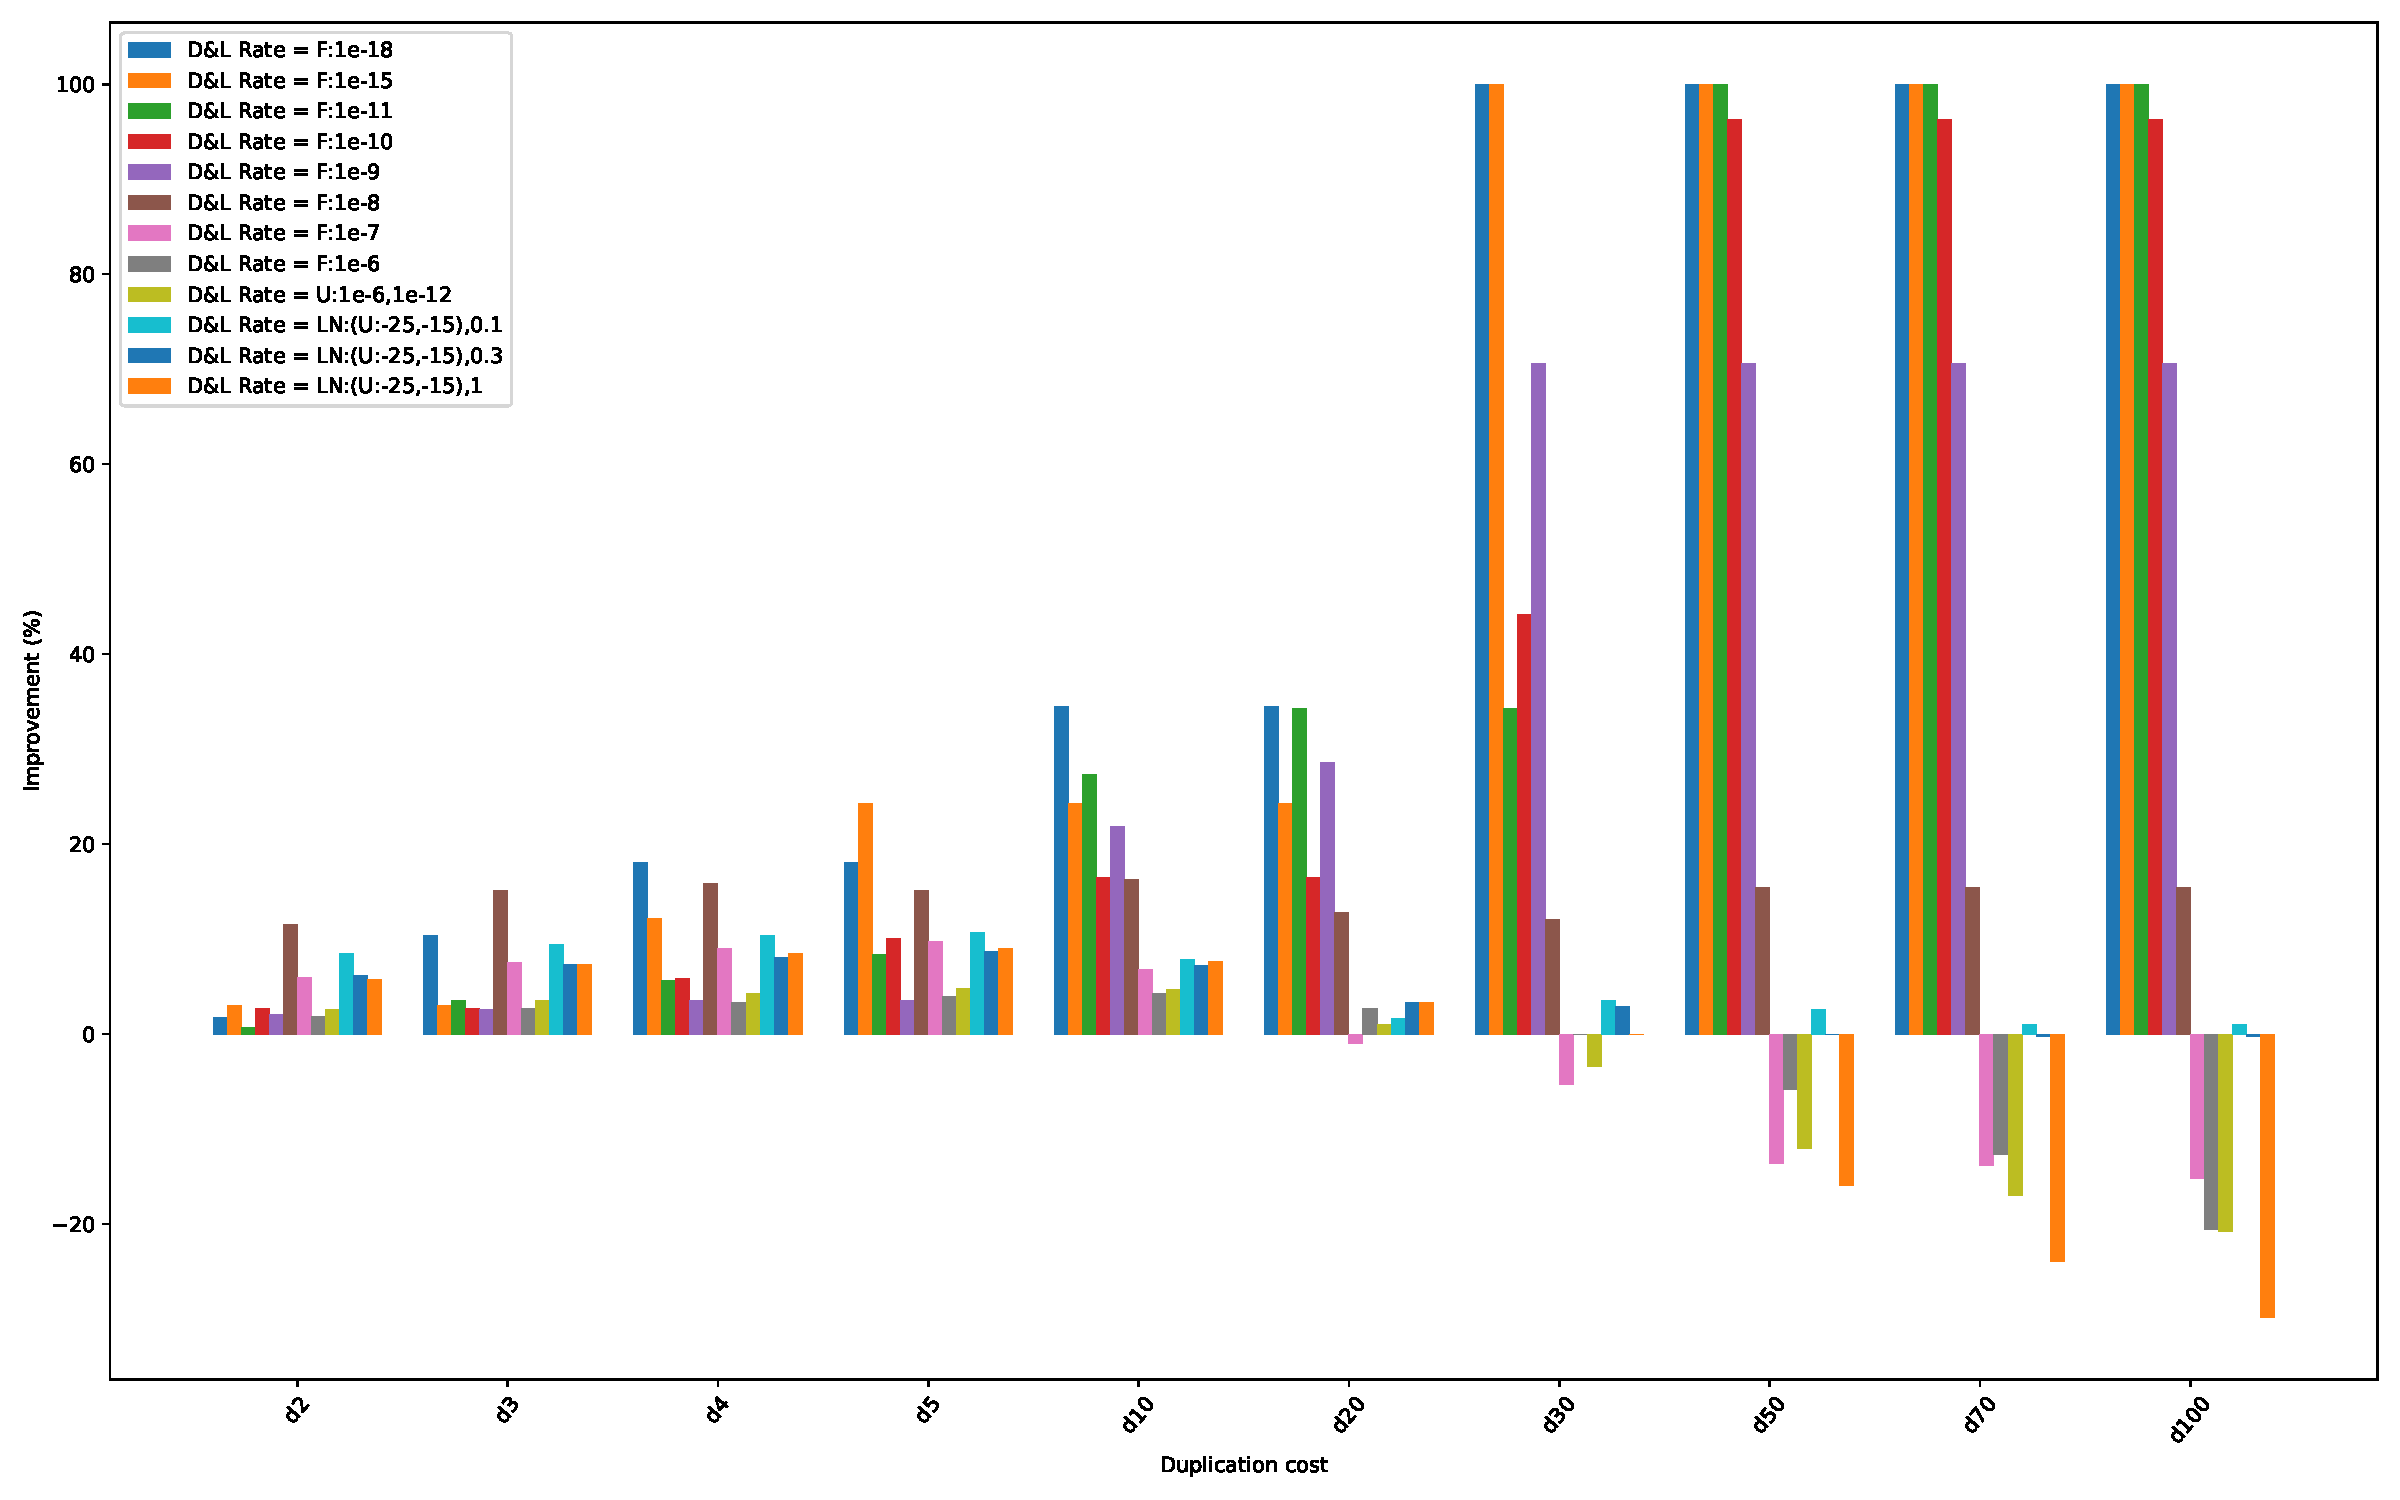
\includegraphics[width=1\textwidth]{figs/imp_1WGD.pdf}
    \caption{Improvement percentages for SimPhy simulations, each simulation containing exactly one WGD.}
    \label{fig:imp_1wgd}
\end{figure}

\begin{figure}[hbt!]
    \centering
    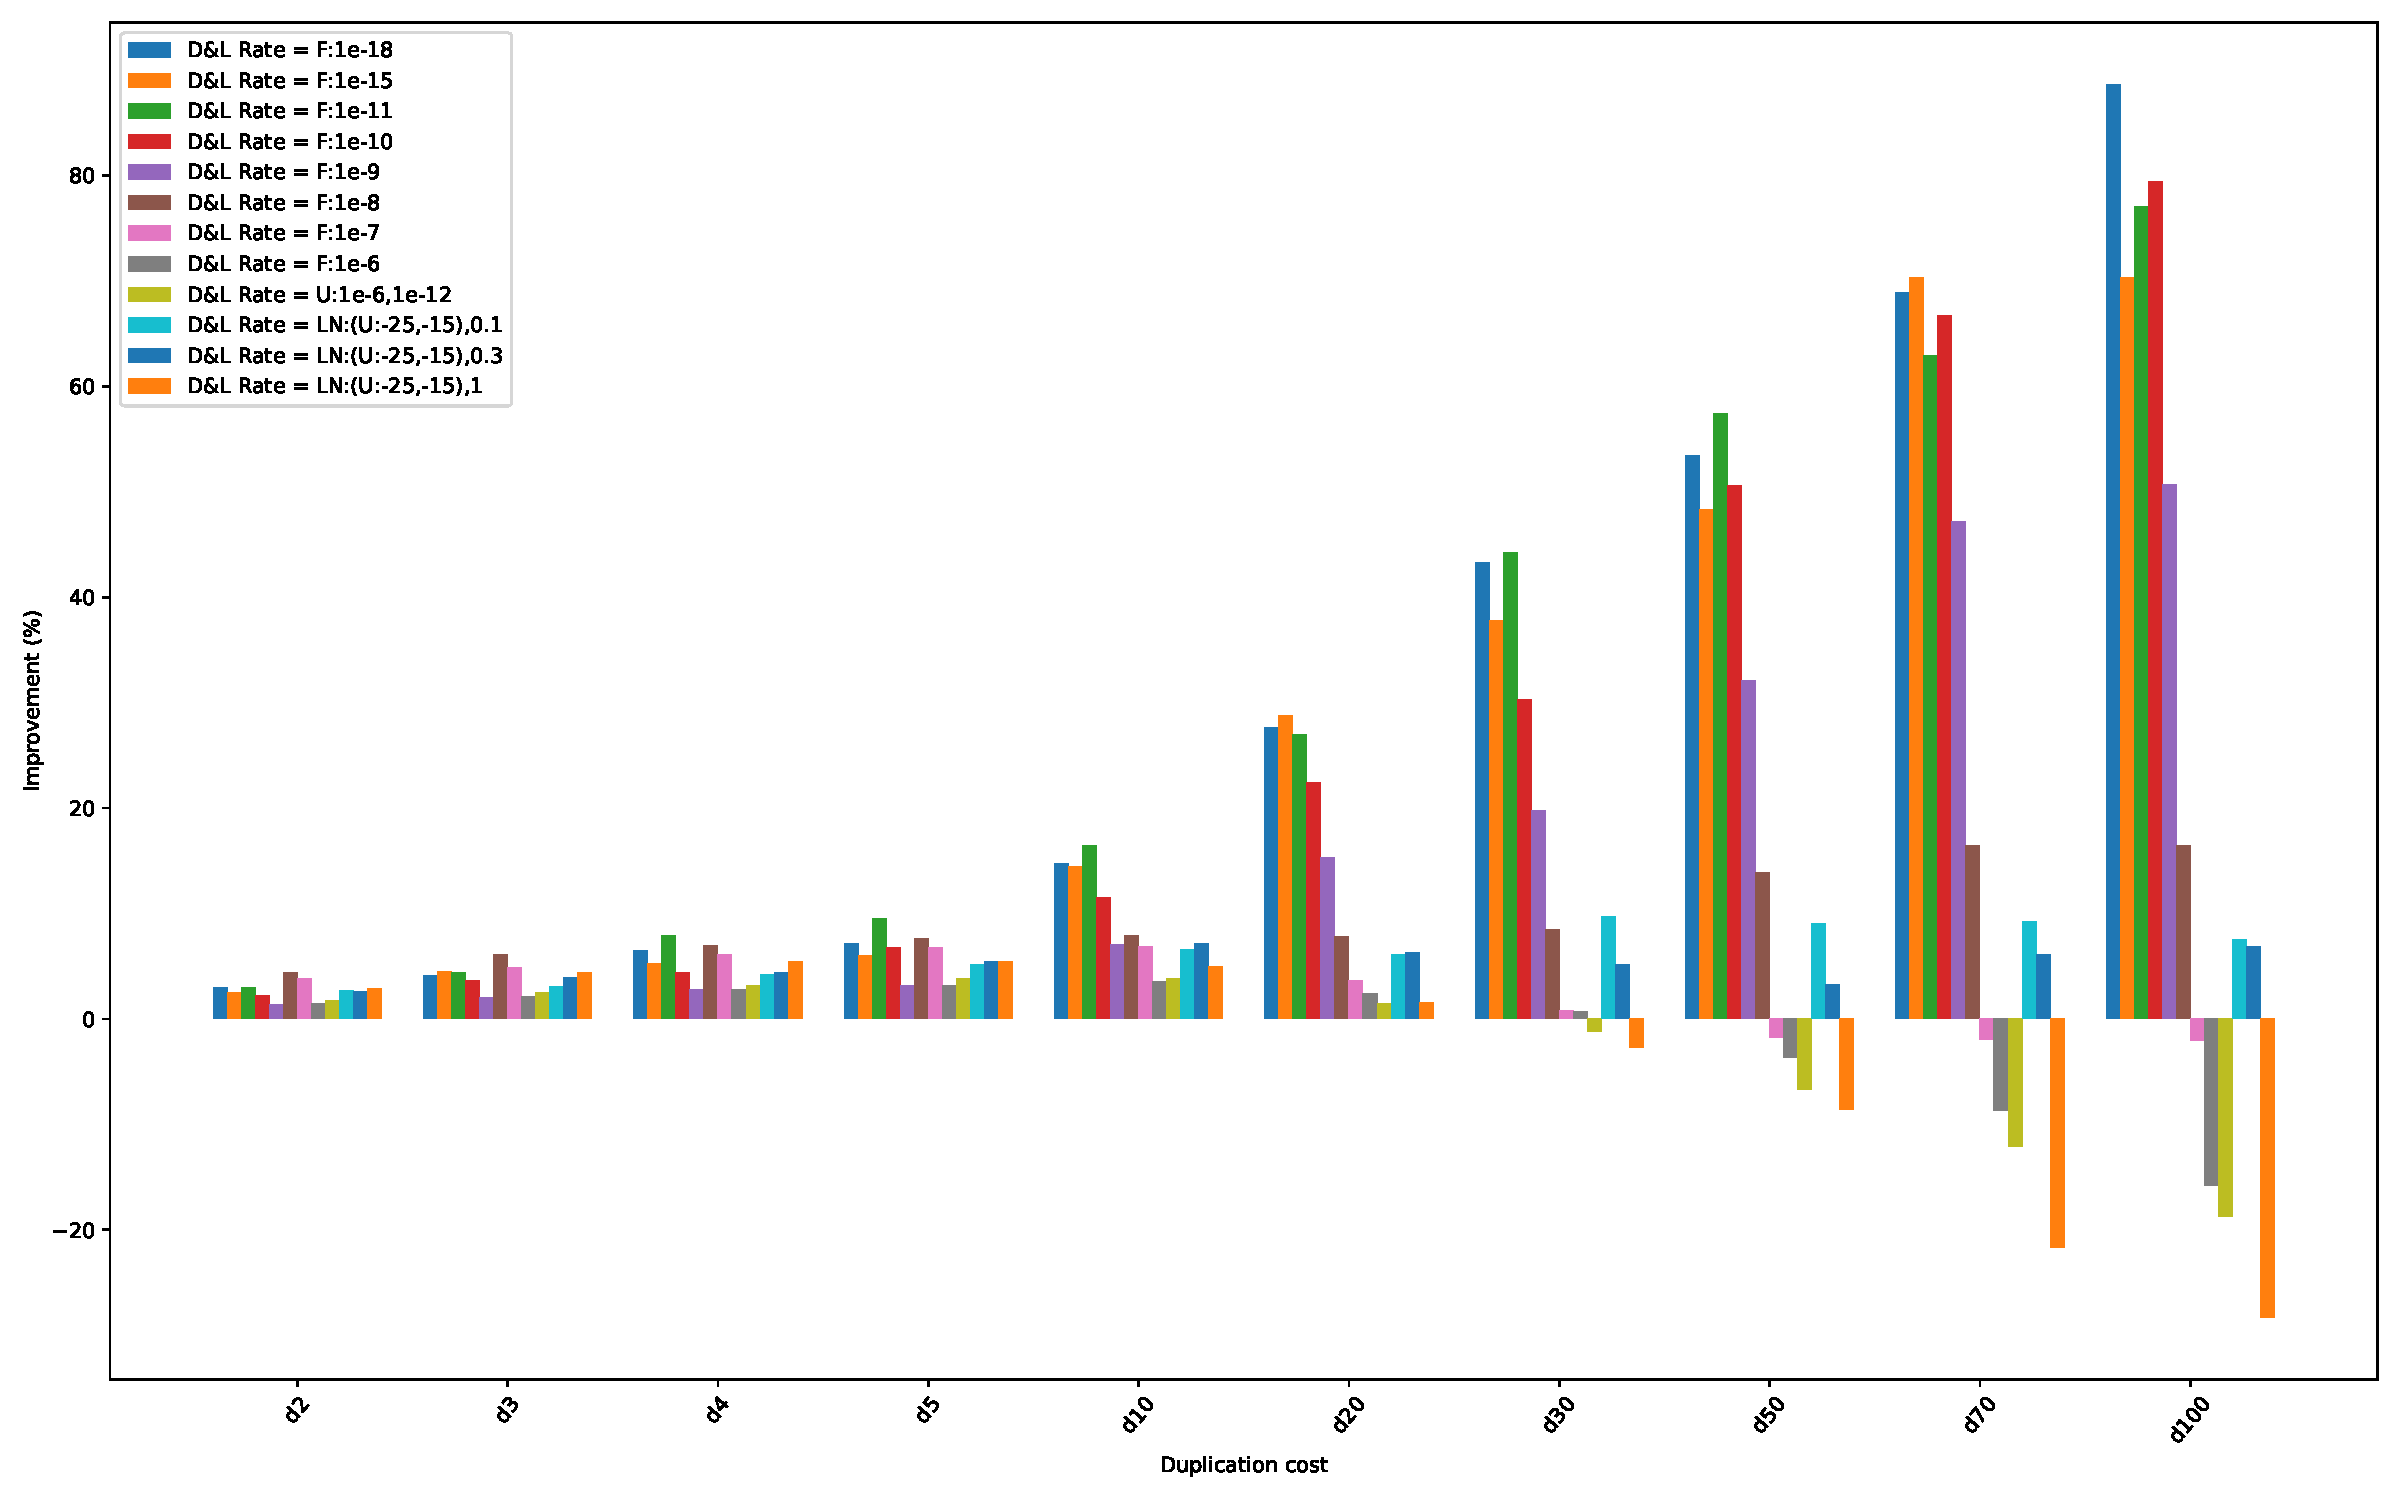
\includegraphics[width=1\textwidth]{figs/imp_2WGD.pdf}
    \caption{Improvement percentages for SimPhy simulations, each simulation containing exactly two WGD.}
    \label{fig:imp_2wgd}
\end{figure}


\begin{figure}[h!]
    \centering
    % First subplot at the top
    \begin{subfigure}[b]{0.48\textwidth}
        \centering
        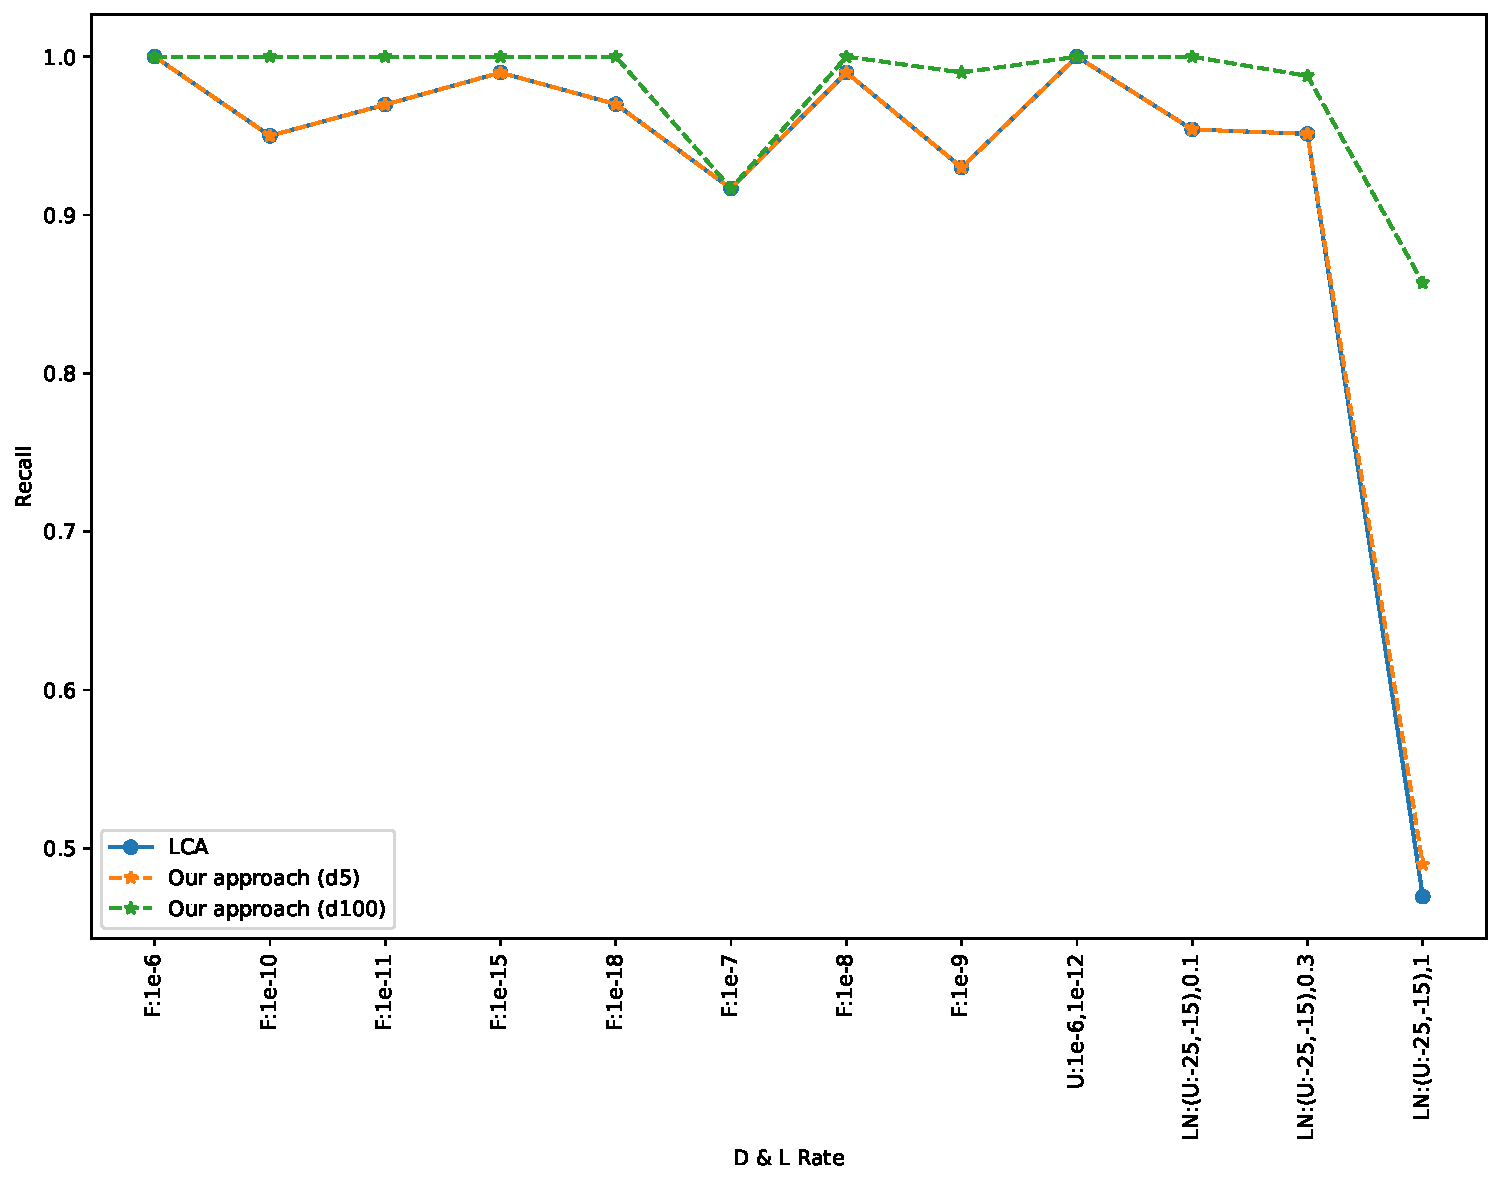
\includegraphics[width=\textwidth]{figs/recall-WGD-t10-t80-Avg.pdf}
        \caption{Recall of WGD for simulations with 1 WGD, averaged over 100 runs.}
        \label{fig:recall-wgd-1wgd}
    \end{subfigure}
    \hfill
    \begin{subfigure}[b]{0.48\textwidth}
        \centering
        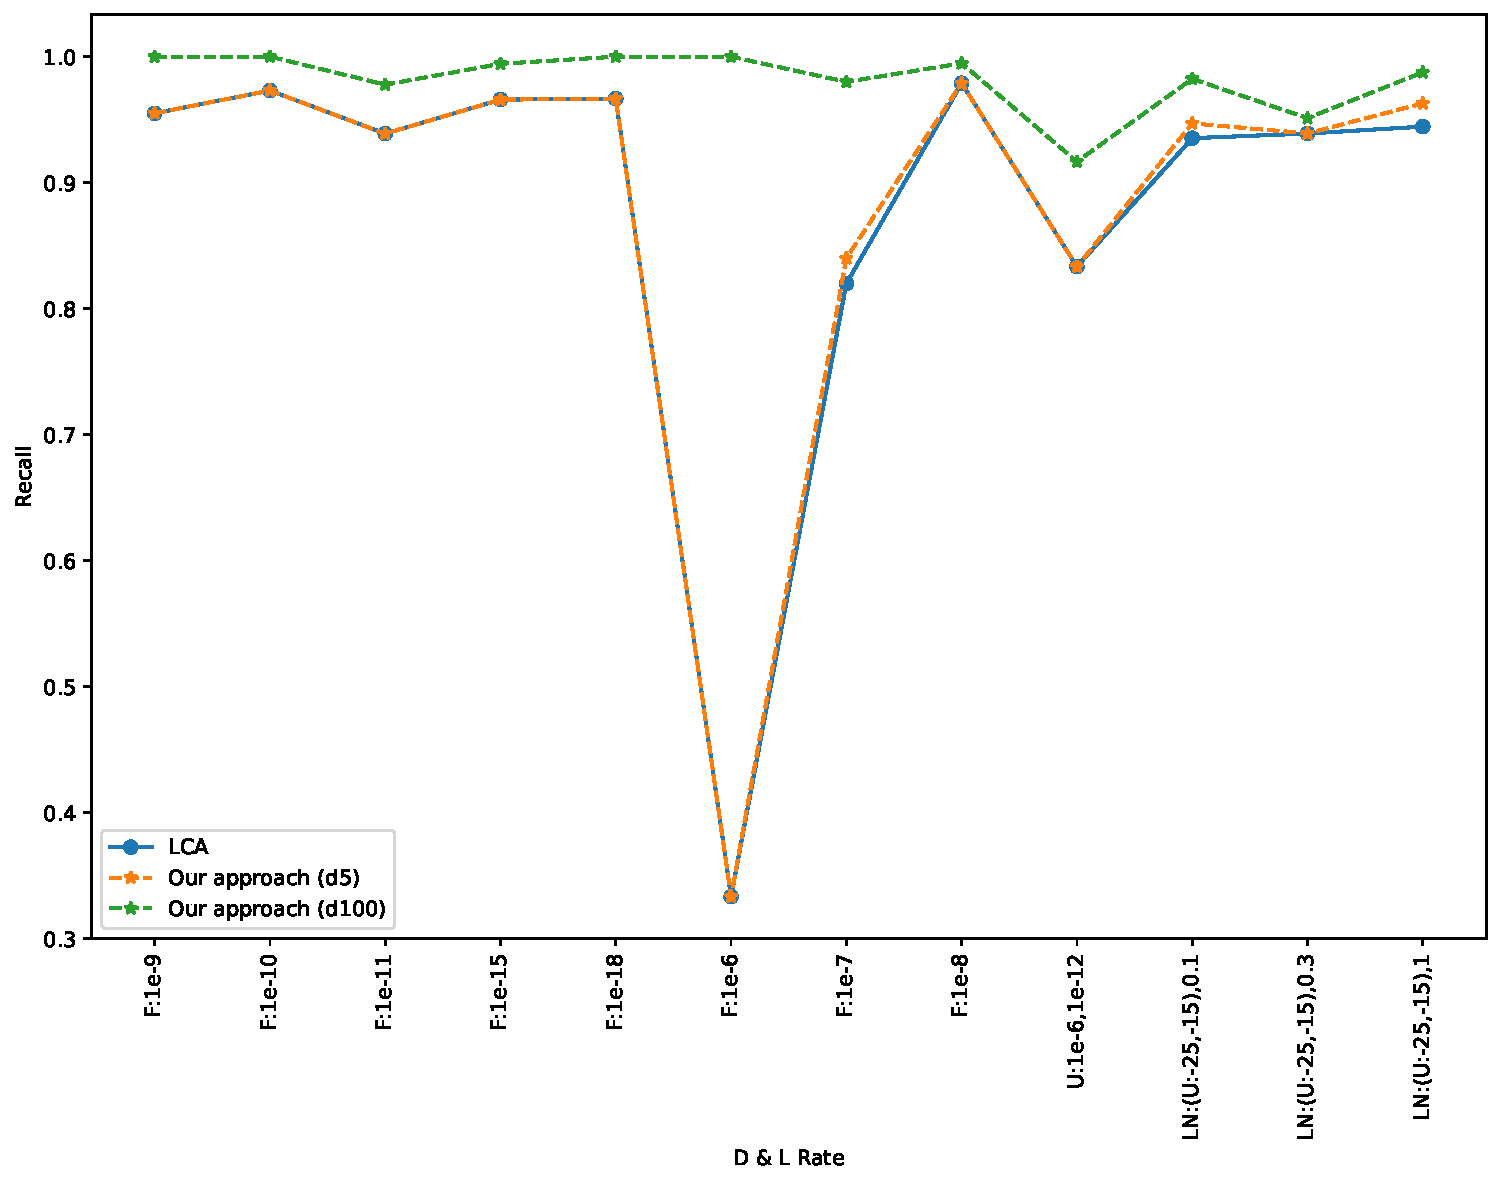
\includegraphics[width=\textwidth]{figs/recall-2W-WGD-t20-t80-Avg.pdf}
        \caption{Recall of WGD for simulations with 2 WGDs, averaged over 100 runs.}
        \label{fig:recall-wgd-2wgd}
    \end{subfigure}
    
    % Two subplots in the second row
    \begin{subfigure}[b]{0.48\textwidth}
        \centering
        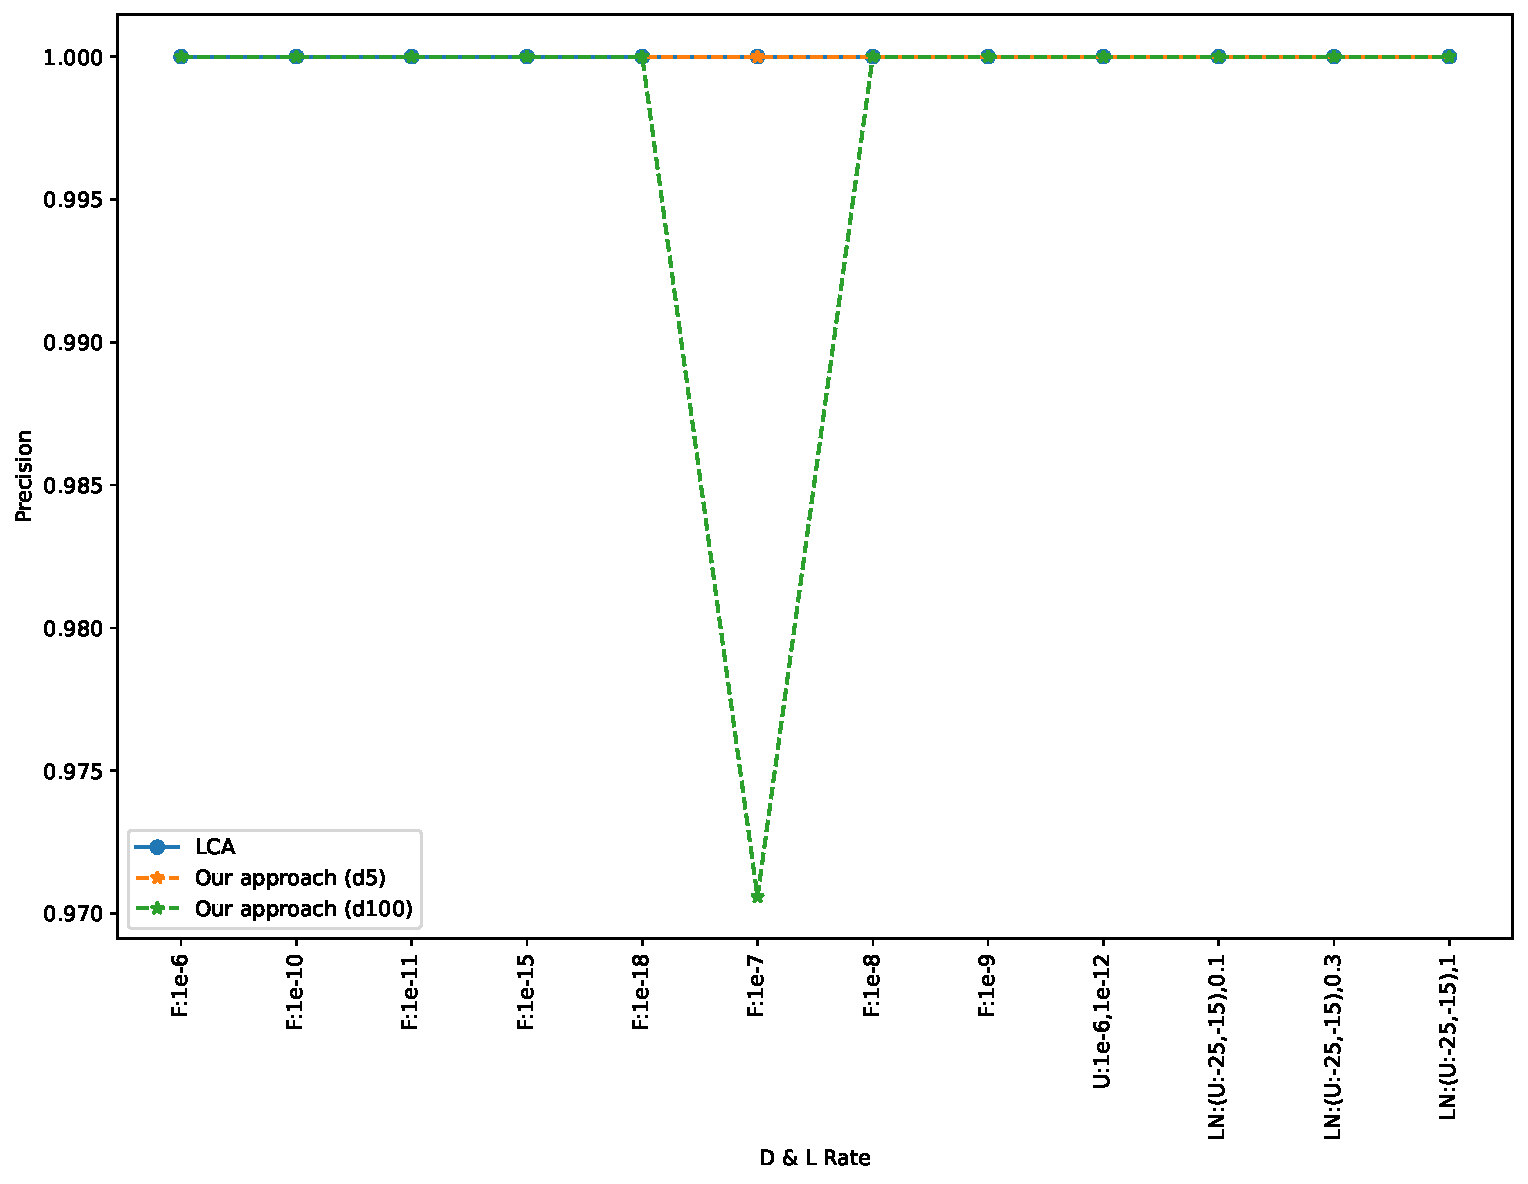
\includegraphics[width=\textwidth]{figs/precision-WGD-t10-t80-Avg.pdf}
        \caption{Precision of WGD for simulations with 1 WGD, averaged over 100 runs.}
        \label{fig:precision-wgd-1wgd}
    \end{subfigure}
    \hfill
    \begin{subfigure}[b]{0.48\textwidth}
        \centering
        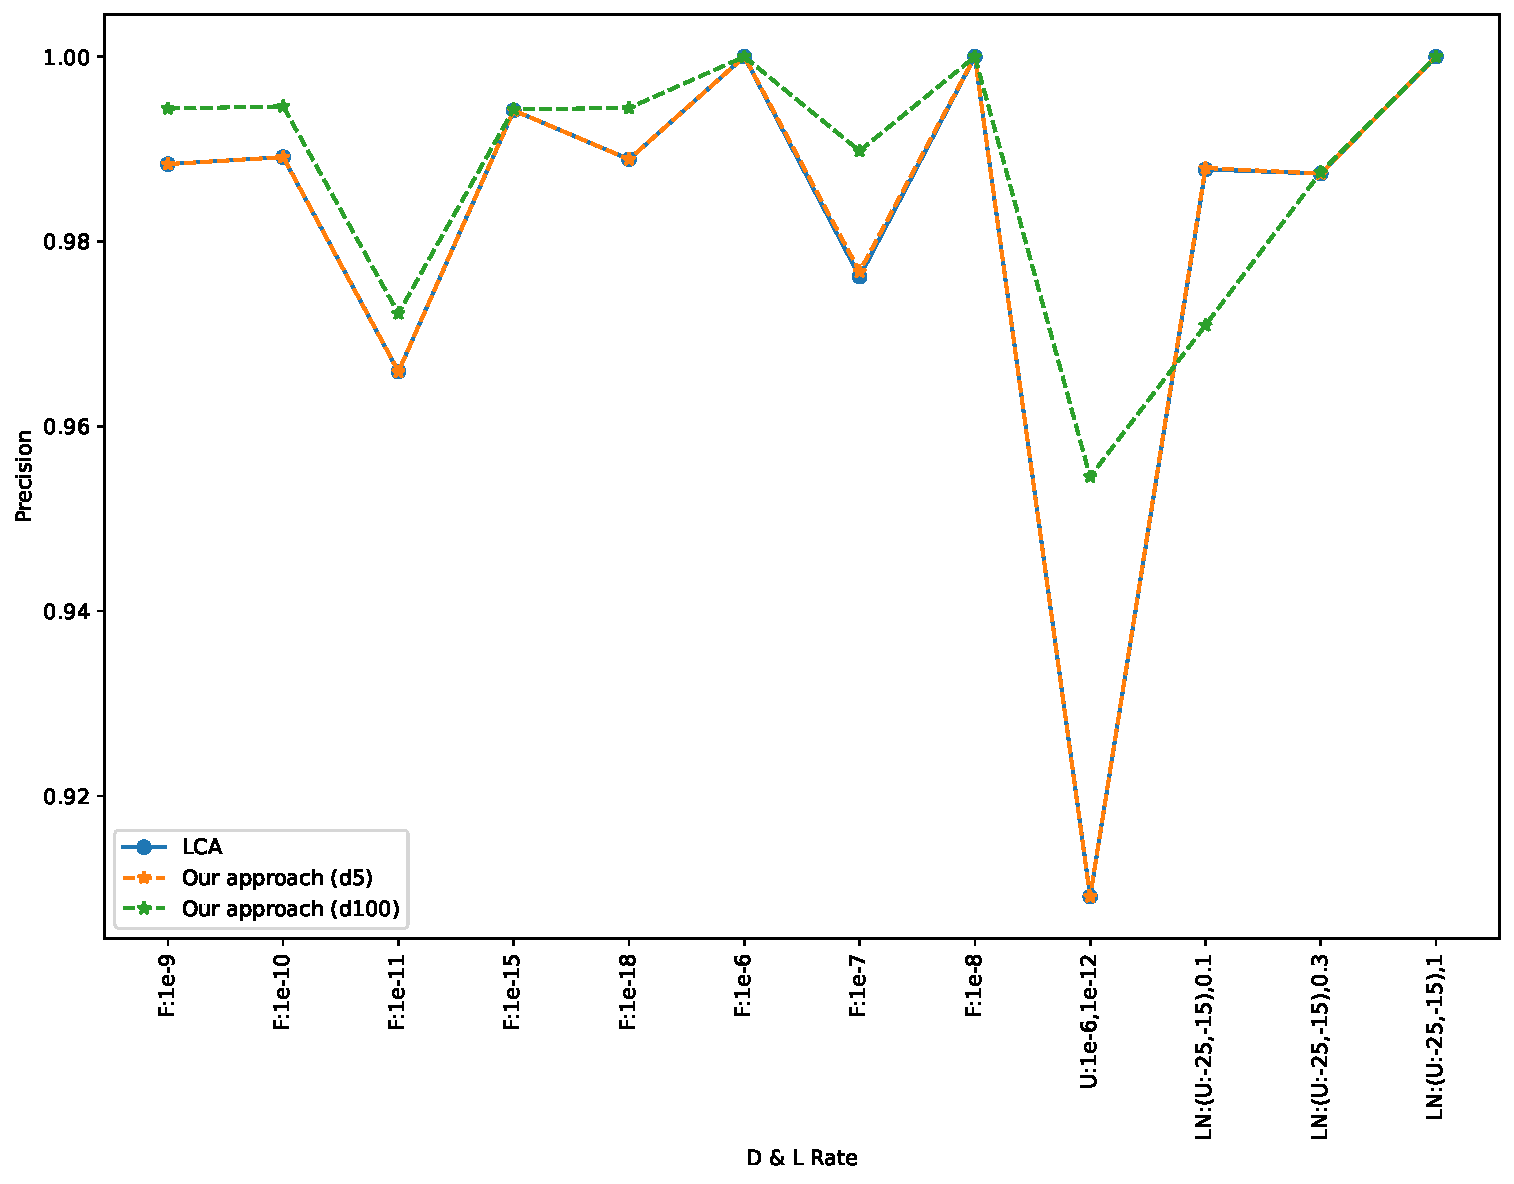
\includegraphics[width=\textwidth]{figs/precision-2W-WGD-t20-t80-Avg.pdf}
        \caption{Precision of WGD for simulations with 2 WGDs, averaged over 100 runs.}
        \label{fig:precision-wgd-2wgd}
    \end{subfigure}
    
    \caption{
Recall and Precision metrics for detecting Whole Genome Duplication (WGD) events in simulations containing either one or two WGDs, analyzed under varying duplication and loss rates. Each result is an average derived from 100 simulation runs, ensuring reliability and robustness of the findings. Subfigure (a) shows the Recall metric for simulations with a single WGD, while subfigure (b) presents the Recall for simulations with two WGDs. Subfigures (c) and (d) display the Precision metrics for simulations with one and two WGDs, respectively.
    }
    \label{fig:recall-precision-wgd}
\end{figure}


\subsection{Results on real datasets}

\ml{[describe datasets we used, with references, and show differences between us and lca.]}
\subsection{Eukaryotes}
In Figur \ref{fig:guigo} ...


\begin{figure}[h!]
    \centering

    % Two subplots in the second row
    \begin{subfigure}[b]{0.48\textwidth}
        \centering
        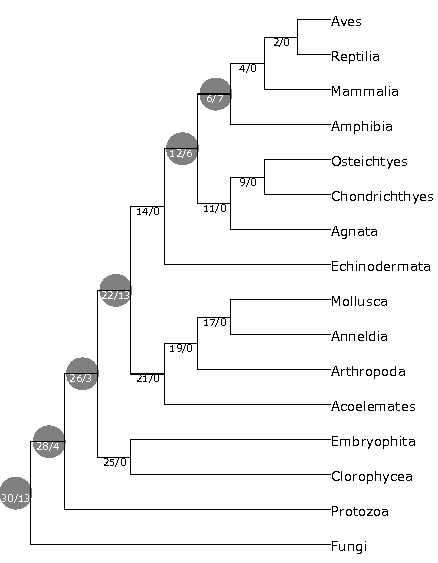
\includegraphics[scale=0.7]{figs/guigo_lca.pdf} % Scale down the image
        \caption{Segmental duplications detected by LCA (gray circles).}
        \label{fig:guigo-lca}
    \end{subfigure}
    \hfill
    \begin{subfigure}[b]{0.48\textwidth}
        \centering
        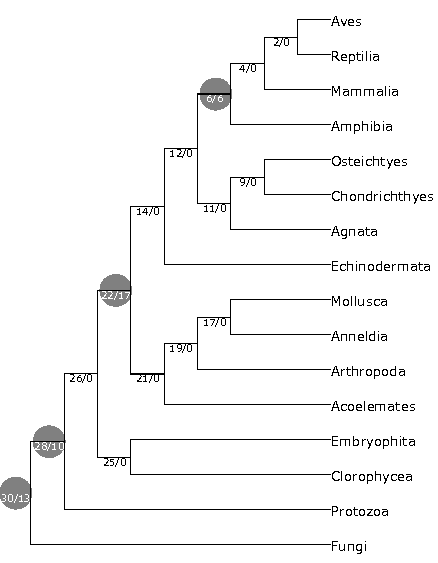
\includegraphics[scale=0.7]{figs/guigo_greedy70.pdf} % Scale down the image
        \caption{Segmental duplications detected by our algorithm ($\delta=50$, $\lambda=1$) shown as gray circles.}
        \label{fig:guigo-greedy}
    \end{subfigure}
    
    \caption{
        Species tree of 16 eukaryotes studied by Guigó et al for 53 gene trees. Each node is labeled with two numbers (a/b), where a is the node ID and b is the count of gene trees supporting duplications in that species.
    }
    \label{fig:guigo}
\end{figure}

\subsection{Yeast}
In Figure \ref{fig:fungi} ...



\begin{figure}[h!]
    \centering

    % Two subplots in the second row
    \begin{subfigure}[b]{0.48\textwidth}
        \centering
        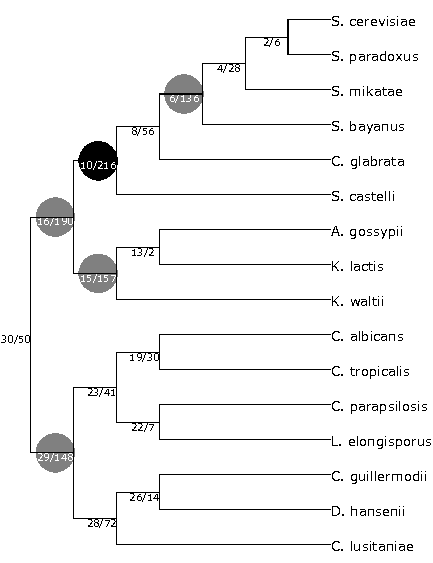
\includegraphics[scale=0.7]{figs/fungi_lca.pdf} % Scale down the image
        \caption{WGD (black cicles) and Segmental duplications (gray circles) detected by LCA.}
        \label{fig:fungi-lca}
    \end{subfigure}
    \hfill
    \begin{subfigure}[b]{0.48\textwidth}
        \centering
        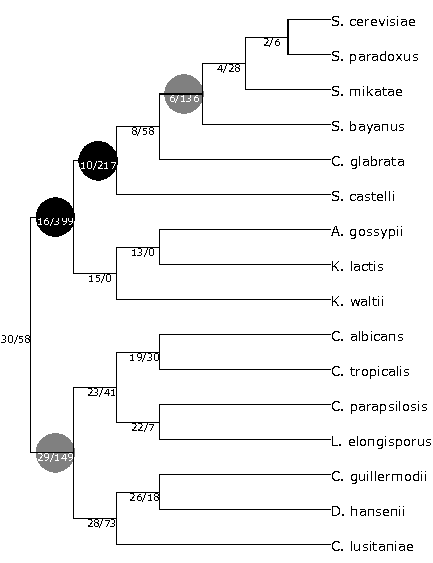
\includegraphics[scale=0.7]{figs/fungi_greedy2000.pdf} % Scale down the image
        \caption{WGD (black cicles) and Segmental duplications (gray circles) detected by our algorithm where $\delta=2000$, $\lambda=1$.}
        \label{fig:fungi-greedy}
    \end{subfigure}
    
    \caption{
        Species tree of 16 yeast species for 2379 gene trees. Each node is labeled with two numbers (a/b), where a is the node ID and b is the count of gene trees supporting duplications in that species.
    }
    \label{fig:fungi}
\end{figure}


\subsection{Salmon}
In Figure \ref{fig:salmon}

\begin{figure}[h!]
    \centering

    % Two subplots in the second row
    \begin{subfigure}[b]{0.48\textwidth}
        \centering
        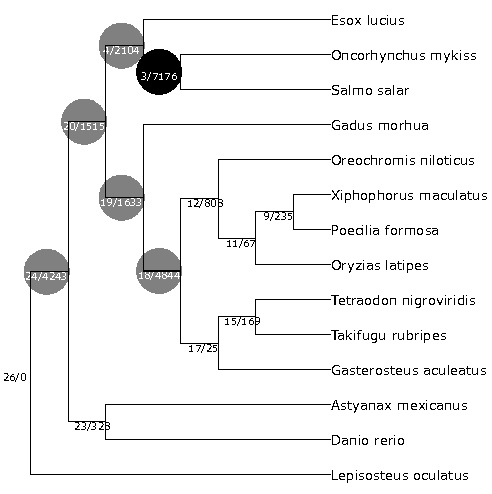
\includegraphics[scale=0.7]{figs/salmon_lca.pdf} % Scale down the image
        \caption{WGD (black cicles) and Segmental duplications (gray circles) detected by LCA.}
        \label{fig:salmon-lca}
    \end{subfigure}
    \hfill
    \begin{subfigure}[b]{0.48\textwidth}
        \centering
        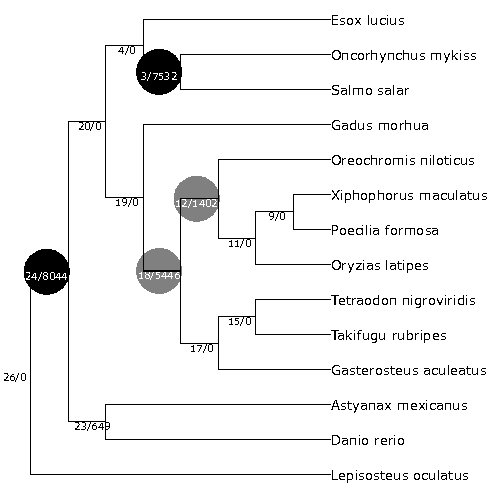
\includegraphics[scale=0.7]{figs/salmon_greedy10000.pdf} % Scale down the image
        \caption{WGD (black cicles) and Segmental duplications (gray circles) detected by our algorithm where $\delta=10000$, $\lambda=1$.}
        \label{fig:salmon-greedy}
    \end{subfigure}
    
    \caption{
        Species tree of atlantic salmon for 12443 gene trees. Each node is labeled with two numbers (a/b), where a is the node ID and b is the count of gene trees supporting duplications in that species.
    }
    \label{fig:salmon}
\end{figure}


\clearpage
\subsection*{Previous stuff}

To begin, we analyze the results from the simulations with one Whole Genome Duplication (WGD) and two WGDs, presented in Figures \ref{fig:imp_1wgd_beforelosses} and \ref{fig:imp_2wgd_beforelosses} respectively. These results are generated under the condition where no losses are applied to the gene trees after the SimPhy simulations, meaning the WGDs remain unaffected by losses. The figures illustrate the improvement percentages across various SimPhy simulations, each subjected to different duplication and loss rates. These results are evaluated under different duplication cost configurations, while keeping the loss cost consistently set to 1.

In the figures, the highest duplication and loss rates tested are $U:1e-6$, $U:1e-12$, and $F:1e-6$, followed by $F:1e-7$. Conversely, the lowest rates are $F:1e-18$, $F:1e-15$, and $F:1e-11$.

In most cases, the LCA mapping outperforms our approach. This is because, when no losses affect the WGDs, the ancestors in the gene trees can be correctly mapped to their respective species, creating an optimal scenario for the LCA method. Additionally, as the duplication cost increases in our approach, it tends to map the gene tree nodes to higher-level species, leading to a decrease in the improvement percentage.

\begin{figure}[hbt!]
    \centering
    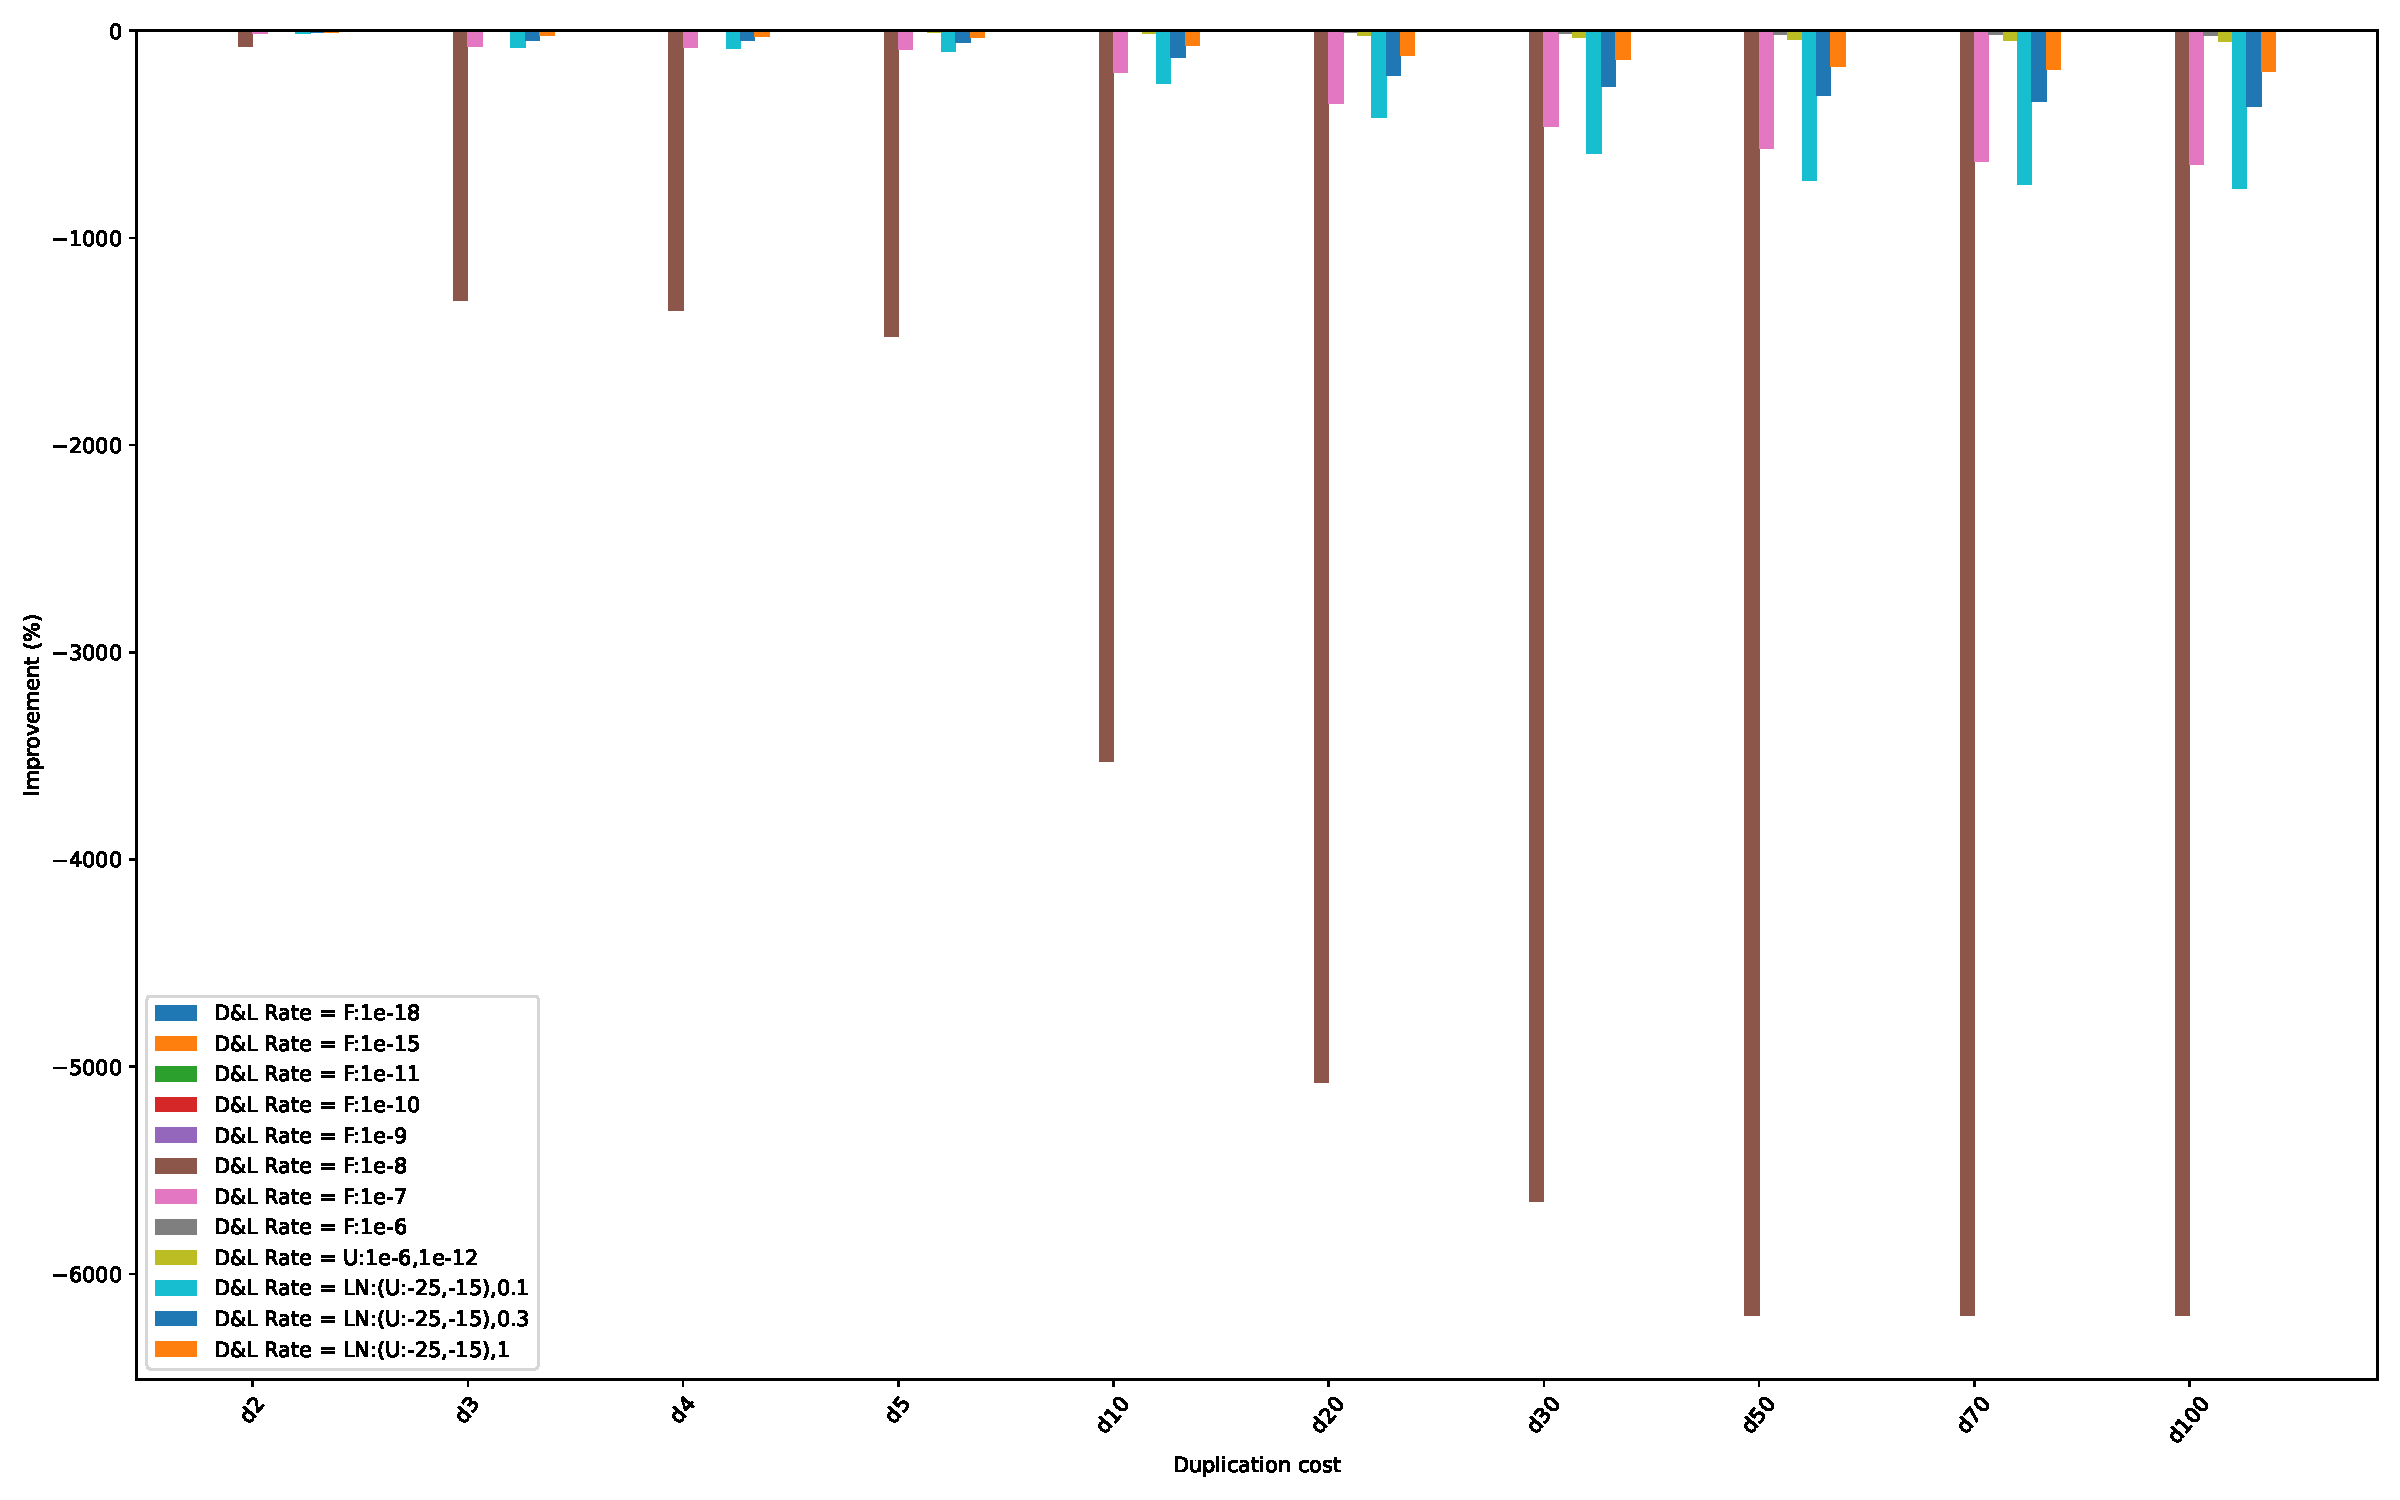
\includegraphics[width=1\textwidth]{figs/imp-1WGD-beforelosses.pdf}
    \caption{Improvement percentages for SimPhy simulations with varying duplication and loss rates. In the legend, "F" represents Point (fixed value) distribution, "U" represents Uniform distribution, and "LN" represents LogUniform distribution. Each simulation includes exactly one WGD event, with no losses applied to the gene trees after the SimPhy simulation.. The x-axis shows the duplication cost used in the algorithm's setup, with the loss cost consistently set to 1.}
    \label{fig:imp_1wgd_beforelosses}
\end{figure}

\begin{figure}[hbt!]
    \centering
    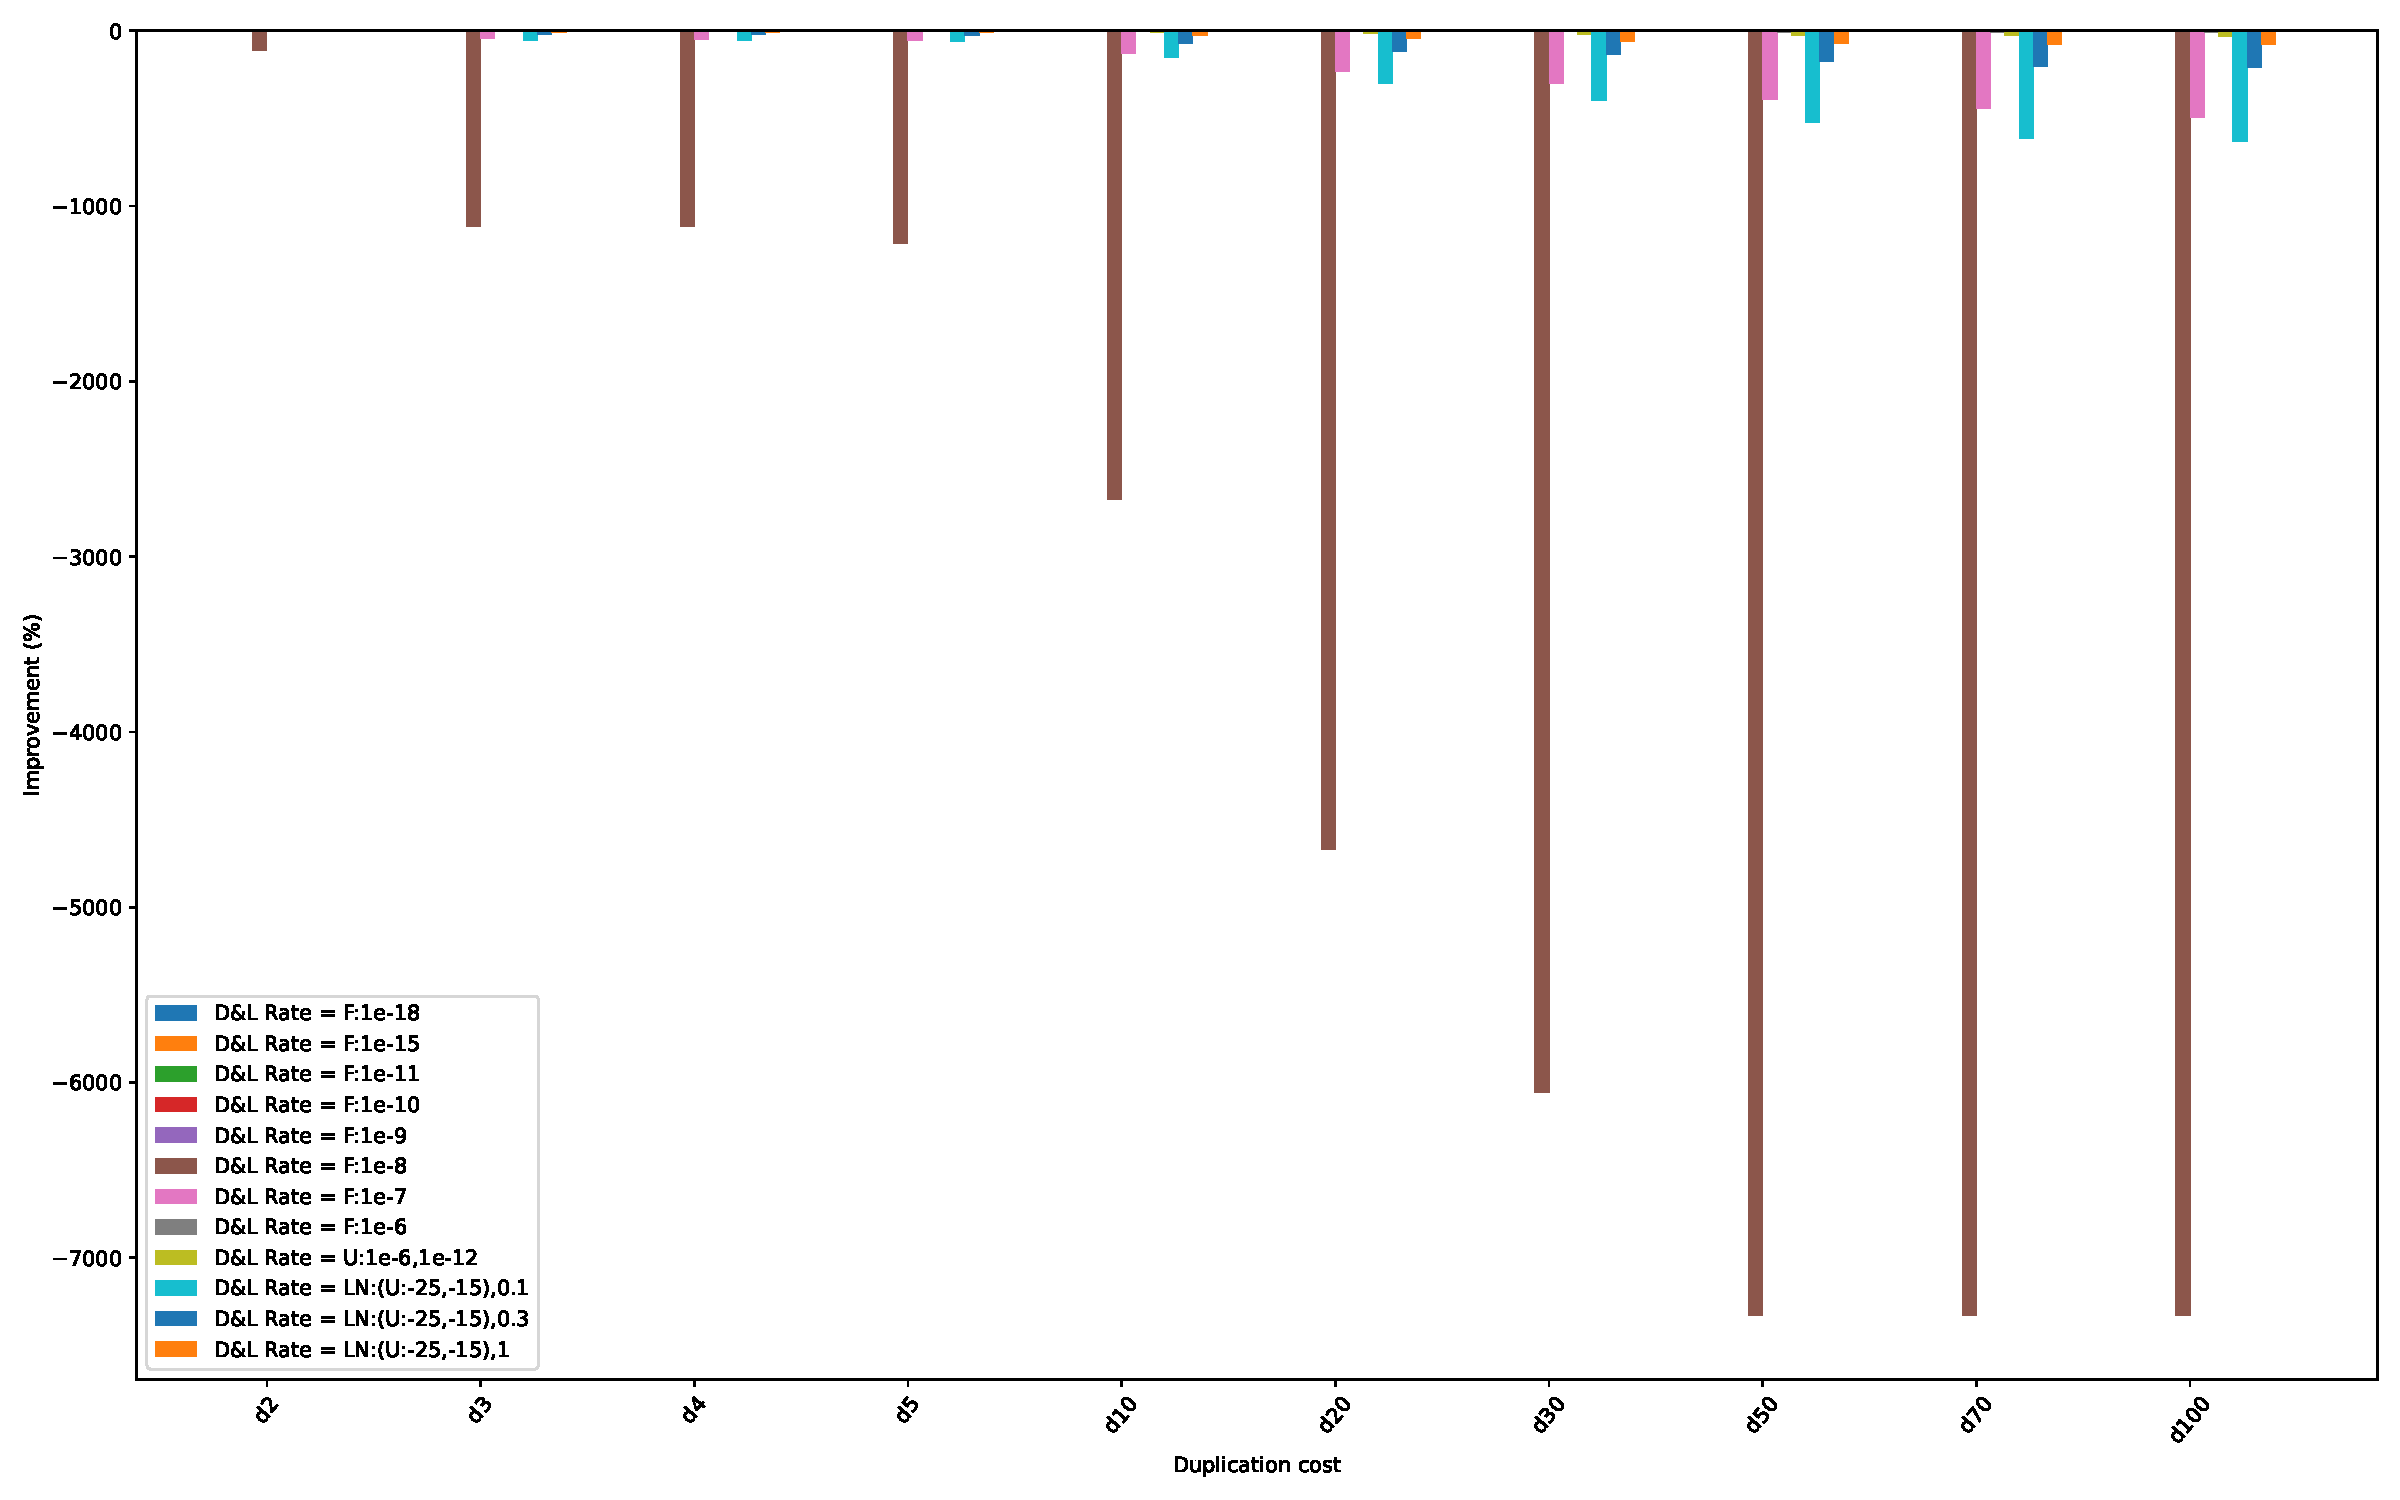
\includegraphics[width=1\textwidth]{figs/imp-2WGD-beforelosses.pdf}
    \caption{Improvement percentages for SimPhy simulations, each containing exactly two WGD events, with no losses applied to the gene trees after the SimPhy simulation.}
    \label{fig:imp_2wgd_beforelosses}
\end{figure}

In Figure \ref{fig:imp_1wgd} and \ref{fig:imp_2wgd}, we examine the results from simulations where losses were applied to the gene trees after SimPhy simulations. The loss rate used is $(n-1)/n$ for each species, where $n$ represents the number of copies of a species. This analysis helps us understand how the application of losses affects the improvement percentages in simulations with one and two WGD events, respectively.

The Figure \ref{fig:imp_1wgd} suggests that with higher duplication costs, the algorithm tends to map duplications to more distant species, leading to greater improvements for lower duplication and loss rates. However, for higher duplication and loss rates, this can result in reduced improvements. Notably, with lower duplication costs (ranging from $d=2$ to $d=20$), the improvements are consistently positive.


\begin{figure}[hbt!]
    \centering
    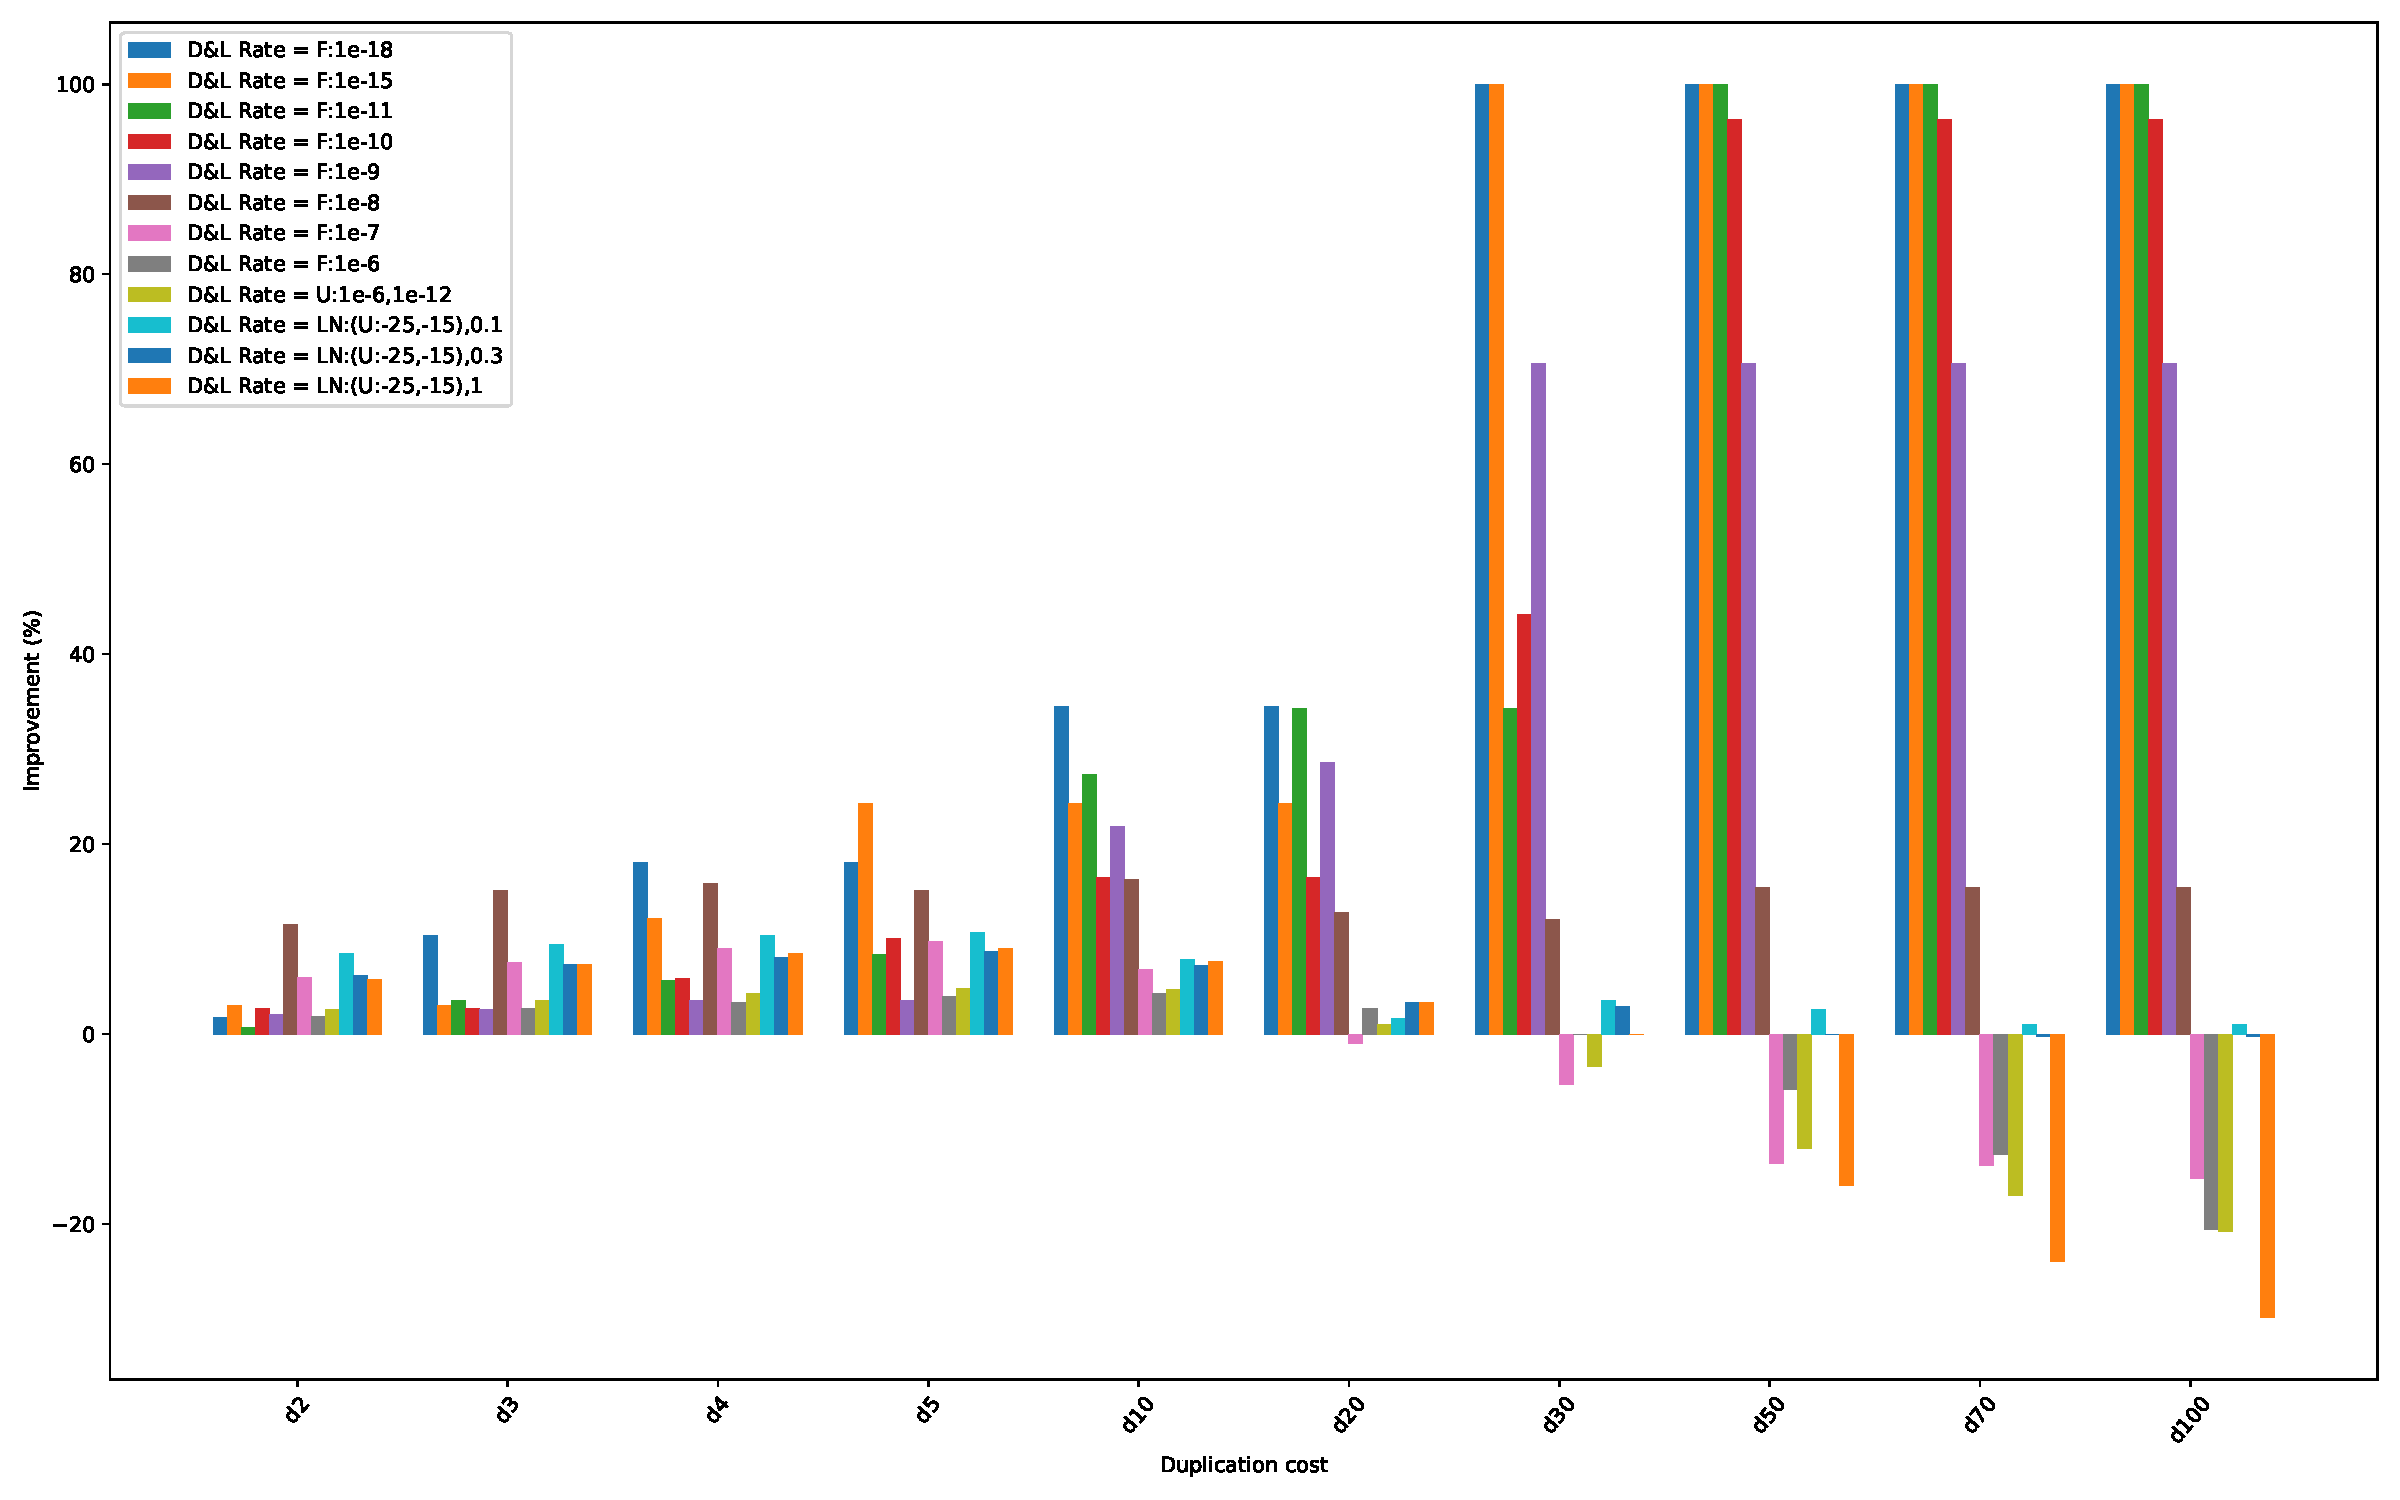
\includegraphics[width=1\textwidth]{figs/imp_1WGD.pdf}
    \caption{Improvement percentages for SimPhy simulations, each containing exactly one WGD events, where losses applied to the gene trees after the SimPhy simulation.}
    \label{fig:imp_1wgd}
\end{figure}

In Figure \ref{fig:imp_2wgd}, we present the improvement percentage results for SimPhy simulations where each simulation includes exactly two WGD events. The trends in this figure are similar to those in Figure \ref{fig:imp_1wgd}, which features simulations with a single WGD, showing similar effects of duplication and loss rates, as well as duplication cost. However, with two WGDs, the improvements tend to increase compared to Figure \ref{fig:imp_1wgd}. This is likely because the influence of random (non-tandem) duplications is reduced in our algorithm with a higher number of WGDs.

\begin{figure}[hbt!]
    \centering
    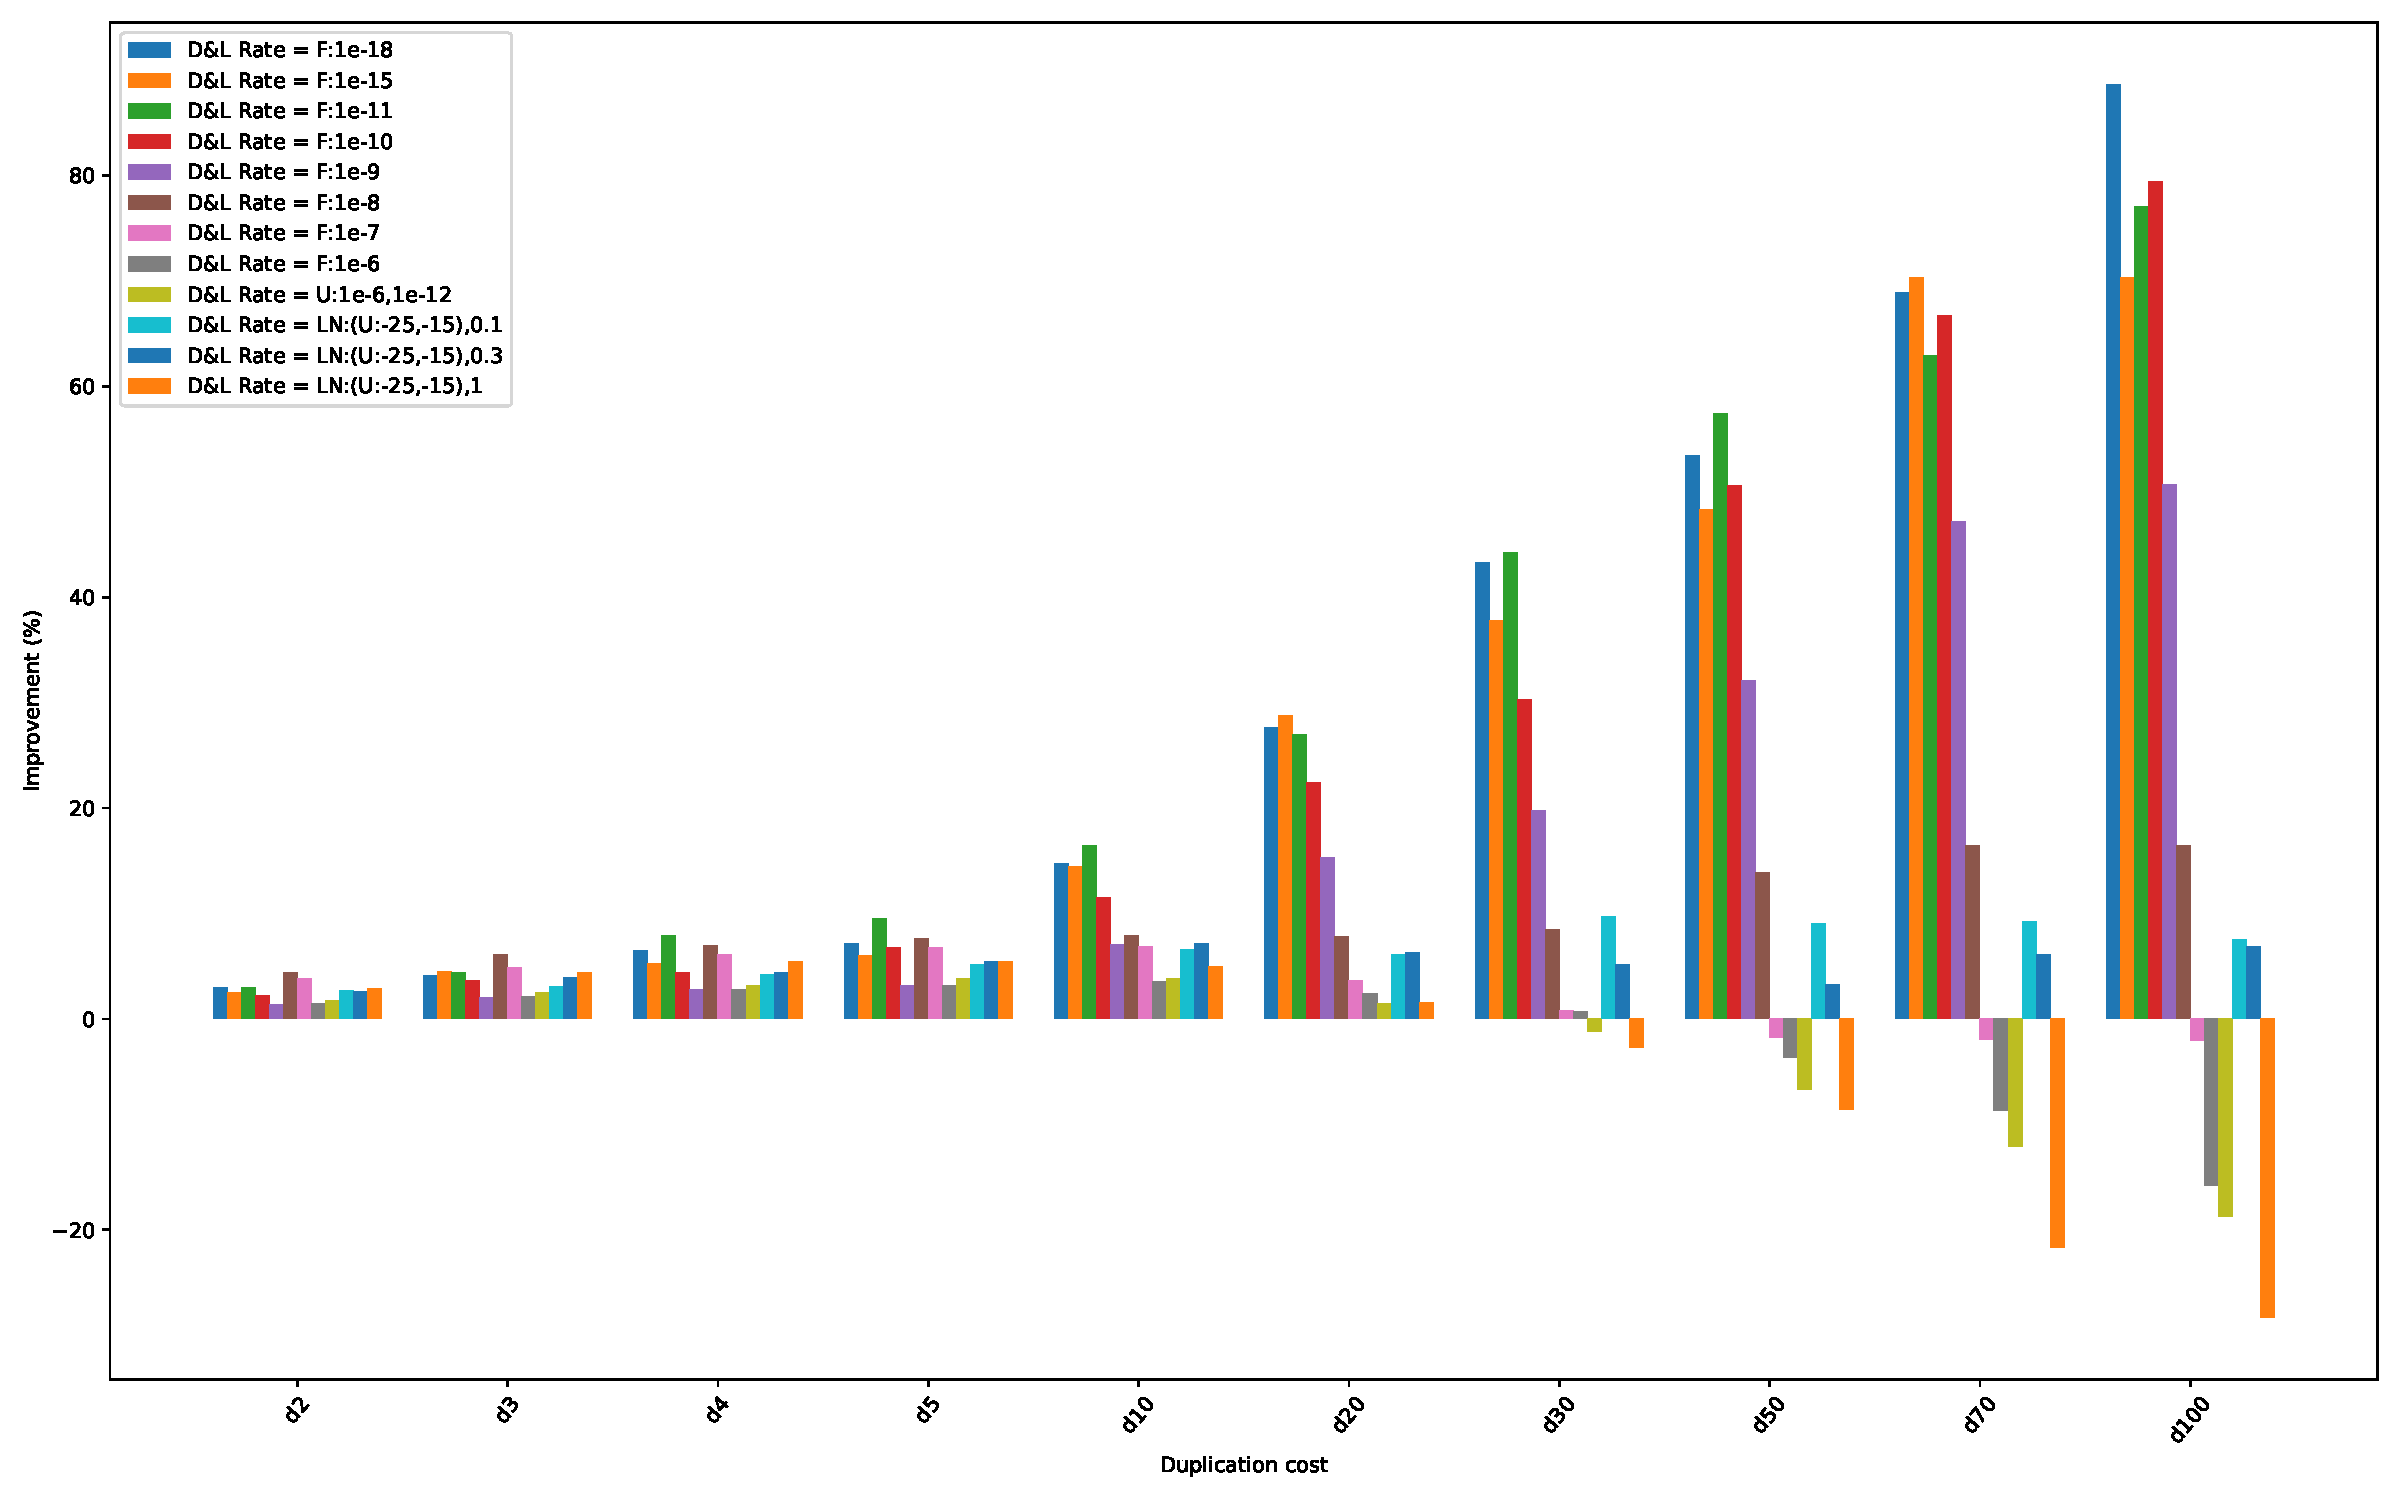
\includegraphics[width=1\textwidth]{figs/imp_2WGD.pdf}
    \caption{Improvement percentages for SimPhy simulations, each containing exactly two WGD events, where losses applied to the gene trees after the SimPhy simulation.}
    \label{fig:imp_2wgd}
\end{figure}

We also explored two additional versions of our algorithm. In the first variant, we disabled down moves (including bulk down moves), allowing only up moves to occur. This approach focuses on finding the best moves from the available up moves. The second variant, referred to as the stochastic version, calculates the total cost change for each possible move. It then uses a Boltzmann distribution to determine the probability of each move being selected like:

$$
\text{p}_i = \text{exp} \left(- \frac{\Delta C_i}{\text{T}}\right)
$$

where $\text{p}_i$ represents the probability of move $i$, $\Delta C_i$ denotes the total cost change associated with move $i$, and $\text{T}$ is the temperature parameter, set to 1. This probability formula allows us to weigh moves based on their cost changes, assigning higher probabilities to moves that result in greater reductions in total cost.

After computing the probabilities for all possible moves, we use a weighted random selection function to choose one move. This ensures that moves with higher probabilities are more likely to be selected. The stochastic algorithm performs this process for 2000 moves and returns the mapping that results in the lowest total cost out of these 2000 moves.

In Figure \ref{fig:imp_1wgd_allalg} and \ref{fig:imp_2wgd_allalg}, which present results for simulations with one and two WGDs, respectively, we compare the performance of three different versions of our algorithm, all using a duplication cost of 5. For scenarios with low duplication and loss rates, the version of our algorithm that disables down moves demonstrates superior performance. This improved performance can be attributed to the fact that with minimal losses, consistently mapping to higher species yields better results in terms of path distances. In these cases, avoiding down moves prevents unnecessary complexity and maintains more accurate mappings. However, for other duplication and loss rates, the three versions of the algorithm exhibit similar improvement percentages. This indicates that, under varying conditions, the advantage of disabling down moves may diminish, leading to comparable performance across the different algorithm versions.


\begin{figure}[hbt!]
    \centering
    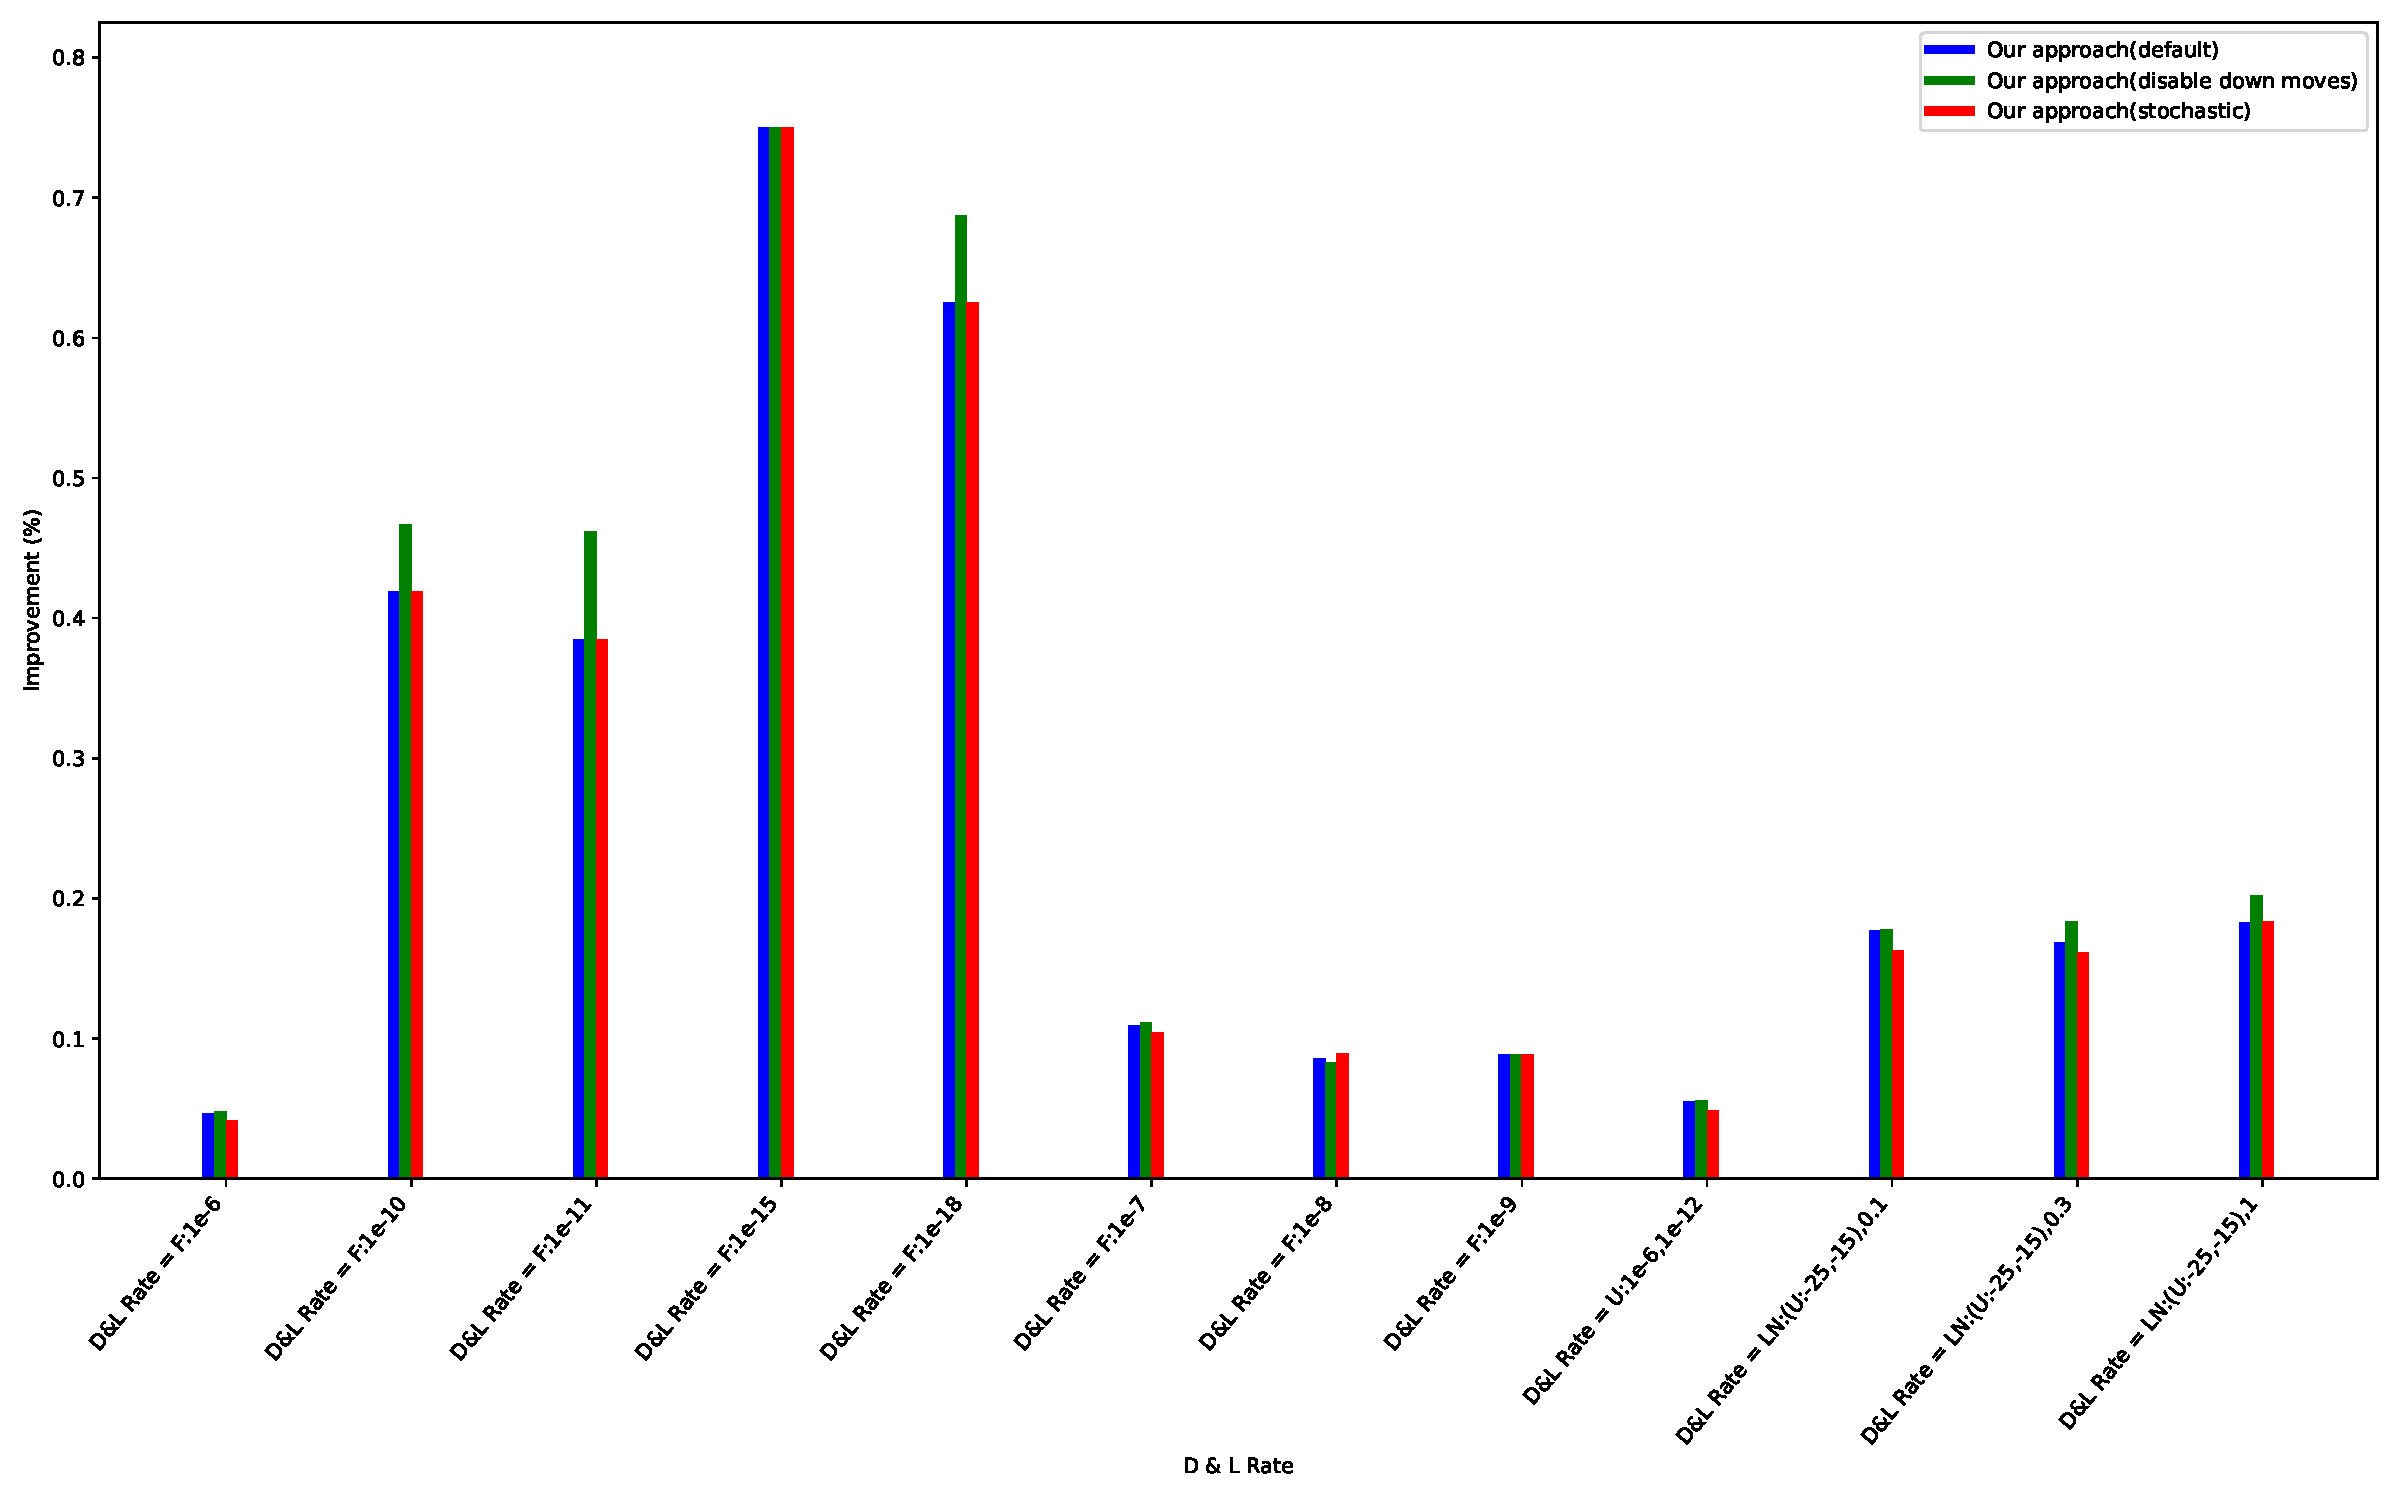
\includegraphics[width=1\textwidth]{figs_theory/imp_1WGD_allalgo_d5.pdf}
    \caption{Comparison of improvement percentages across three different versions of our algorithm for SimPhy simulations, each containing exactly one WGD events. In these simulations, losses were applied to the gene trees after the SimPhy simulation. This figure highlights how each algorithm version performs under varying conditions of duplication and loss rates.}
    \label{fig:imp_1wgd_allalg}
\end{figure}

\begin{figure}[hbt!]
    \centering
    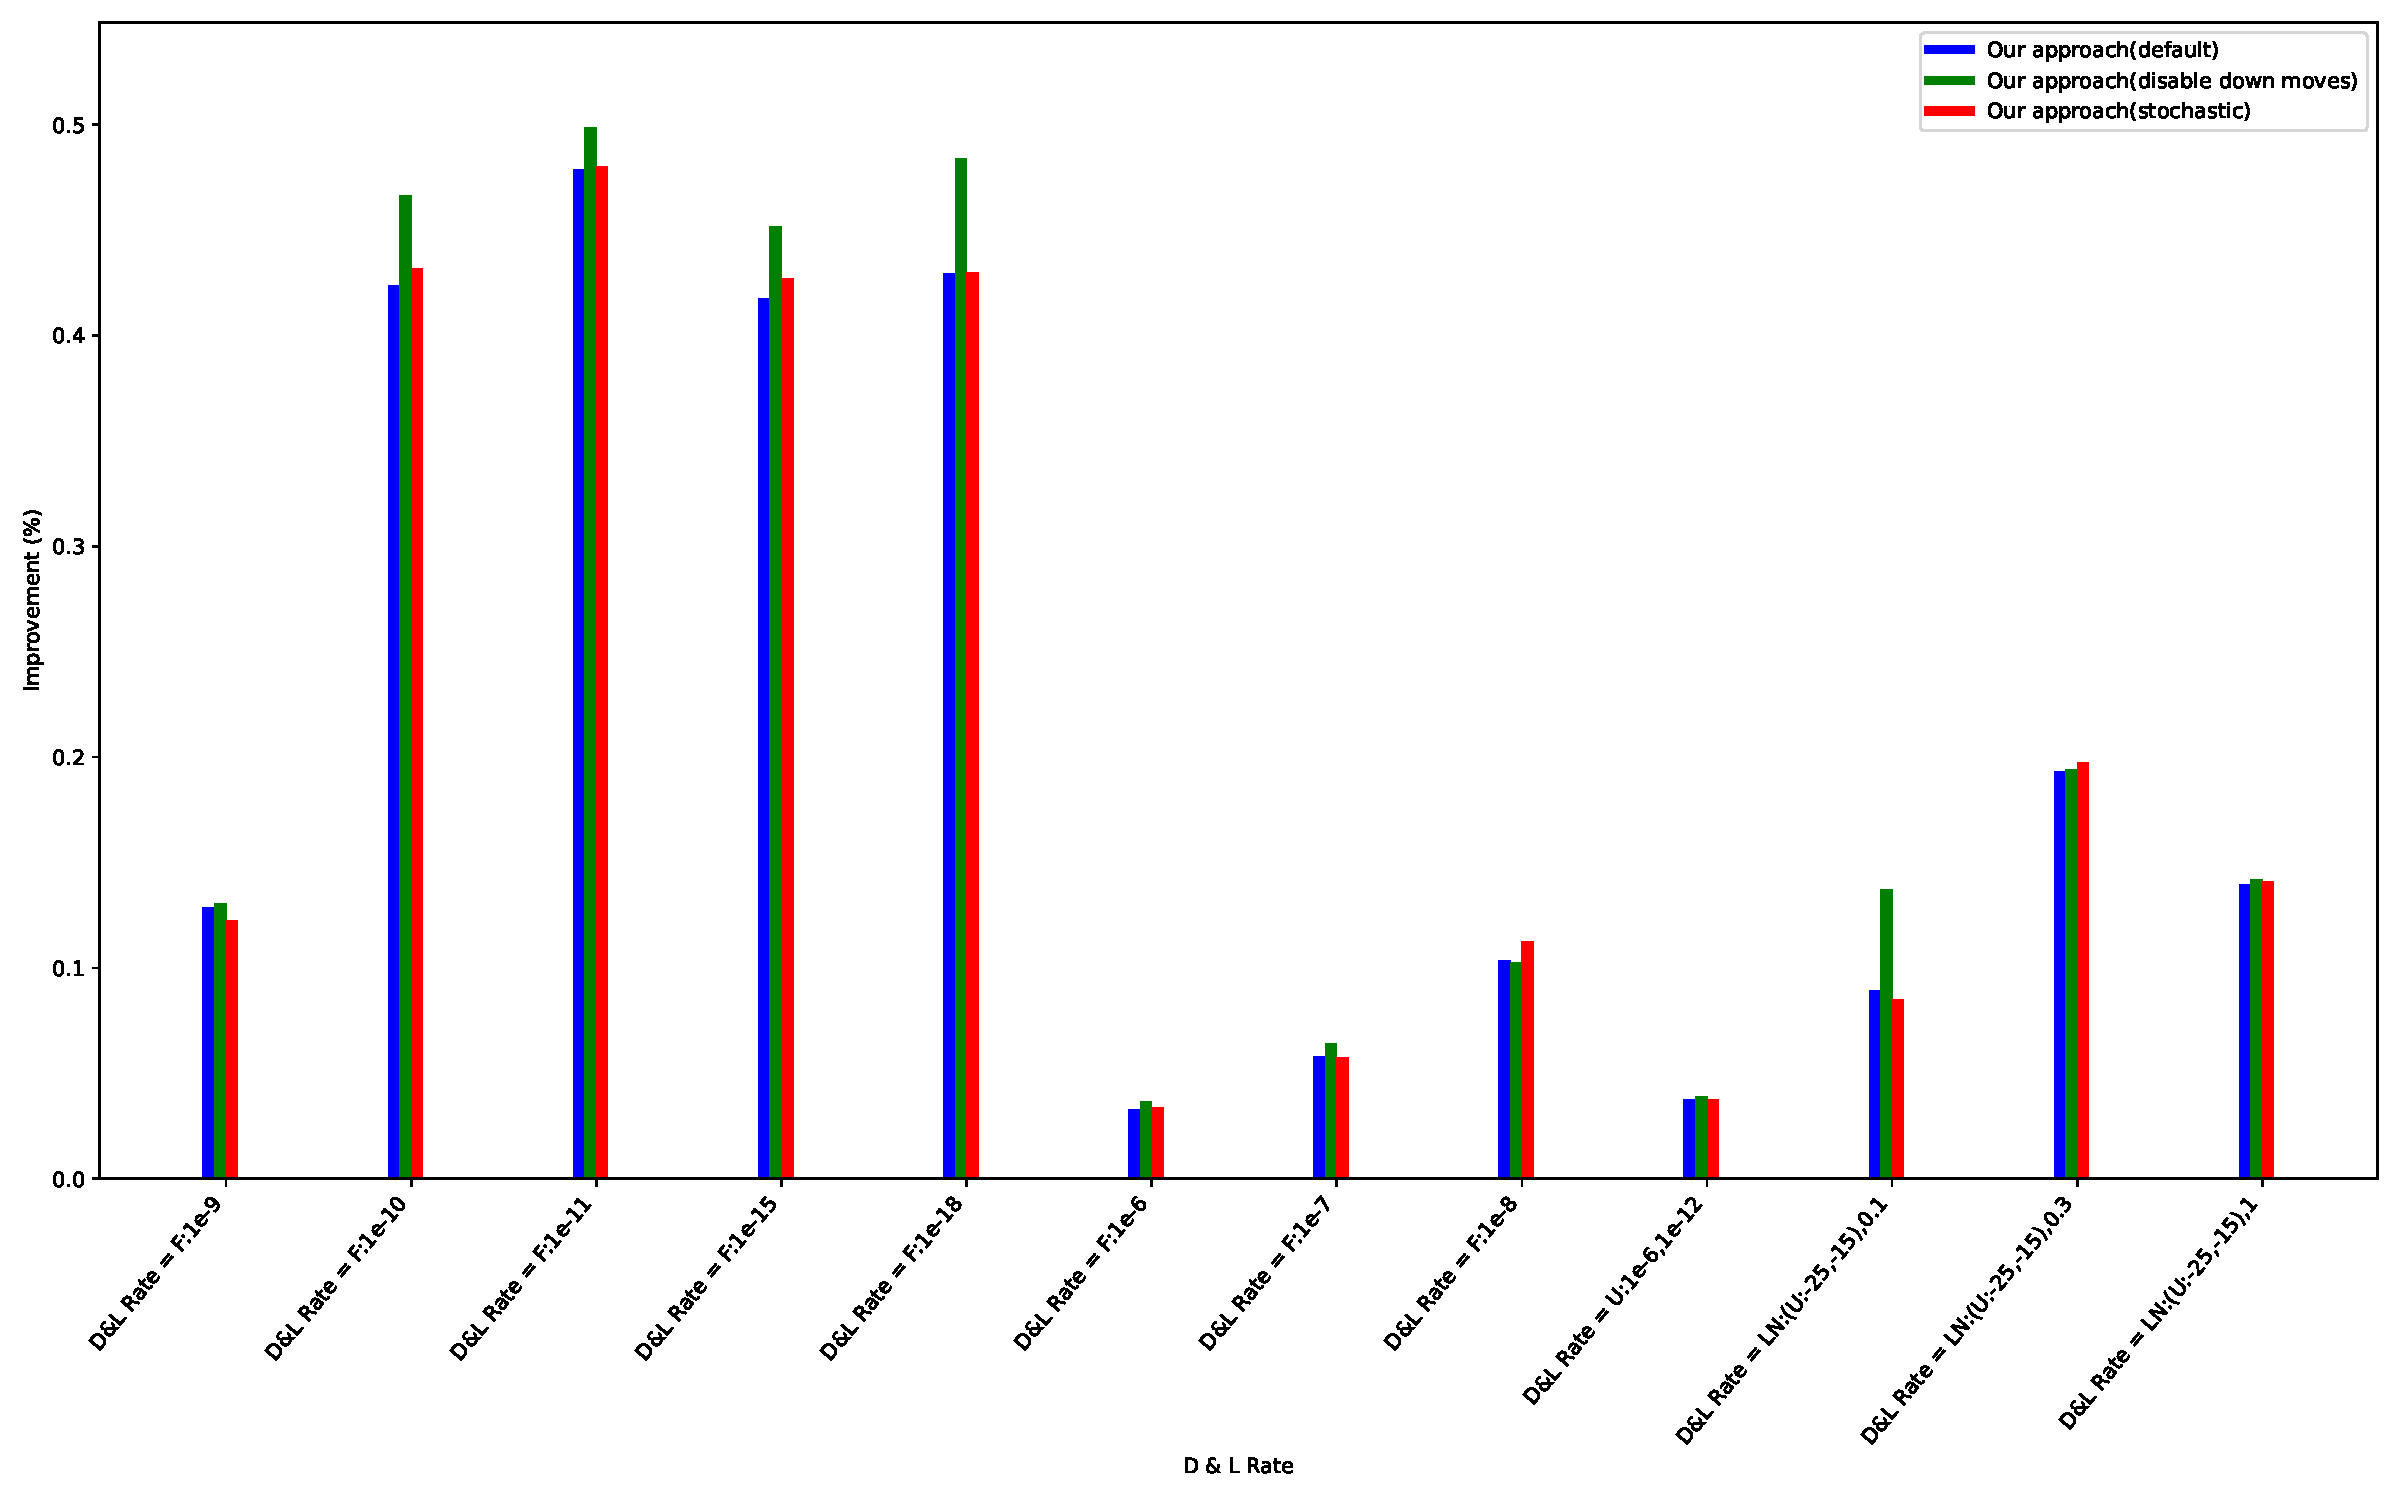
\includegraphics[width=1\textwidth]{figs_theory/imp_2WGD_allalgo_d5.pdf}
    \caption{Comparison of improvement percentages across three different versions of our algorithm for SimPhy simulations, each containing exactly two WGD events. In these simulations, losses were applied to the gene trees after the SimPhy simulation.}
    \label{fig:imp_2wgd_allalg}
\end{figure}


\subsection{Amplitudes}

The next metric we define is amplitude. For this metric, we examine each species across all gene trees, and the number of gene trees in which a species has a duplication is referred to as the number of $Gis$.

$$
\text{Amplitude(s)} = Gis(algorithm) - Gis(SimPhy)
$$

Here, $\text{Amplitude}(s)$ represents the amplitude value for species $s$, $Gis(\text{algorithm})$ is the number of gene trees in which species $s$ has a duplication according to the algorithm (either LCA or our approach), and $Gis(\text{SimPhy})$ represents the true number of $Gis$ for species $s$.


In Figure \ref{fig:amp}, we visualize the amplitude plot for species from a single simulation with a duplication and loss rate of $F:1e-11$. Subfigure \ref{fig:amp-a} shows the amplitude using the LCA mapping, while \ref{fig:amp-b} and \ref{fig:amp-c} display our approach with duplication costs of 5 and 100, respectively.

As observed in this simulation, there is only one WGD event. In the LCA mapping, the WGD is partially recovered, with some duplications being assigned to one of the descendants of the species (Note: the species on the x-axis are post-ordered).

Our approach with a duplication cost of 5 effectively reduces the noise present in the LCA mapping. When the duplication cost is increased to 100, our method fully recovers all duplications accurately, aligning perfectly with the true mapping. Notably, the Sum value is 0, indicating that the sum of all amplitudes for all species is zero, signifying no discrepancy between our approach and the true mapping.
 
\begin{figure}[h!]
    \centering
    % First subplot at the top
    \begin{subfigure}[b]{0.5\textwidth}
        \centering
        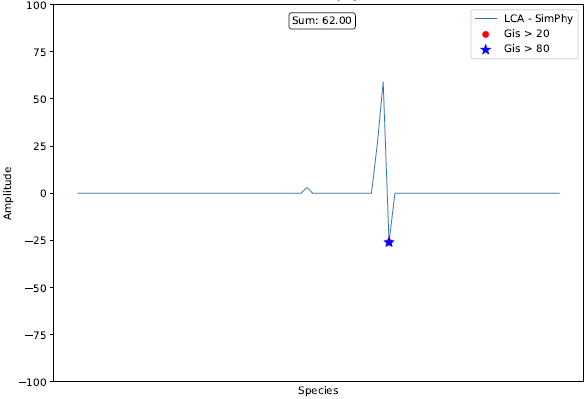
\includegraphics[width=\textwidth]{figs/LCA-amp.PNG}
        \caption{Amplitude plot for species using LCA mapping.}
        \label{fig:amp-a}
    \end{subfigure}
    
    % Two subplots in the second row
    \begin{subfigure}[b]{0.48\textwidth}
        \centering
        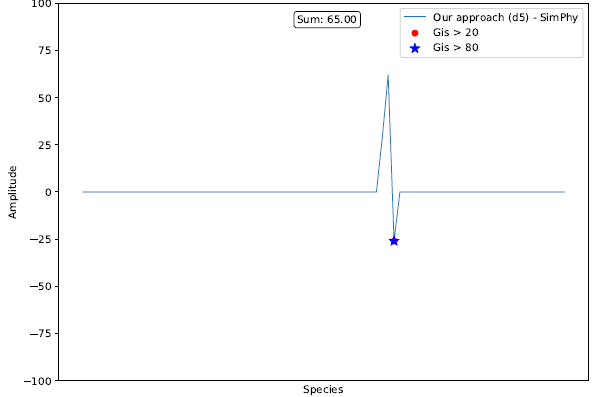
\includegraphics[width=\textwidth]{figs/greedy5-amp.PNG}
        \caption{Amplitude plot for species using our approach with duplication cost $d=5$.}
        \label{fig:amp-b}
    \end{subfigure}
    \hfill
    \begin{subfigure}[b]{0.48\textwidth}
        \centering
        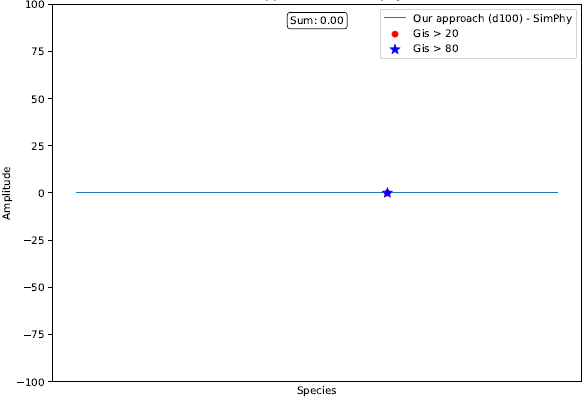
\includegraphics[width=\textwidth]{figs/greedy100-amp.PNG}
        \caption{Amplitude plot for species using our approach with duplication cost $d=100$.}
        \label{fig:amp-c}
    \end{subfigure}
    
    \caption{
    Amplitude plots from a single simulation with duplication and loss rates set to $F:1e-11$. These plots illustrate the differences in the number of duplications across gene trees for each species. We apply thresholds to classify duplication events as either whole genome duplications (WGD) or segment duplications (SD). Specifically, a species with duplications in more than 80\% of gene trees is classified as experiencing a WGD, indicated by a blue star in the figure. Conversely, a species with duplications in more than 20\% but less than 80\% of gene trees is classified as an SD, indicated by a red circle. The Sum value in each plot represents the sum of all y-values, where a positive number indicates that the algorithm identified more duplications than the true number, and a negative number indicates fewer. Therefore, the closer the Sum value is to 0, the more accurate the algorithm is in detecting duplications. This visualization helps to compare the performance of LCA mapping against our approach under different duplication cost settings.
    }
    \label{fig:amp}
\end{figure}





\subsection{Recall and Precision}
In this section, we define Recall and Precision for our approach. To do so, we first need to establish the concepts of True Positives, False Negatives, and False Positives. Additionally, before introducing these measures, it is essential to clarify how we define Whole Genome Duplication (WGD) and Segmental Duplication (SD) within our simulations.

\textbf{Whole Genome Duplication (WGD):} A species is considered to have undergone a WGD if it exhibits duplication in more than 80\% of the gene trees.

\textbf{Segmental Duplication (SD):} A species is considered to have undergone SD if it shows duplication in more than 20\% but less than 80\% of the gene trees.

\textbf{True Positives (TP):} A species is counted as a true positive if it has a WGD in the true simulation and is also identified as having a WGD in our approach or LCA.

\textbf{False Negatives (FN):} A species is counted as a false negative if it has a WGD in the true simulation but is not identified as having a WGD in our approach or LCA.

\textbf{False Positives (FP):} A species is counted as a false positive if it does not have a WGD in the true simulation but is incorrectly identified as having a WGD in our approach or LCA.

The same definitions apply when evaluating SD events.

\textbf{Recall}, also known as sensitivity or true positive rate, is a metric that quantifies the ability of our approach to correctly identify positive instances out of all the actual positive cases. It reflects the completeness of the positive predictions. A high recall indicates that the method successfully captures most of the true positive events, minimizing the number of false negatives.

$$
\text{Recall} = \frac{\text{TP}}{\text{TP+FN}}
$$

\textbf{Precision} measures the accuracy of the positive predictions made by the approach. It is the proportion of true positive cases among all cases predicted as positive. Precision reflects the reliability of the positive predictions, indicating how often the positive predictions are actually correct. A high precision means that when the method predicts a positive case, it is likely to be correct, reducing the occurrence of false positives.

$$
\text{Precision} = \frac{\text{TP}}{\text{TP+FP}}
$$

Finally, since all these metrics—Recall, Precision, and others—are calculated for a single simulation, and we have 100 repeated simulations for each duplication and loss rate in SimPhy, we take the average of these metrics across all 100 simulations for each specific duplication and loss rate. This averaging process allows us to obtain a more robust and reliable estimate of the algorithm's performance, and we can better understand how our approach performs under different conditions and gain insights into the overall trends across varying duplication and loss rates.

\begin{figure}[h!]
    \centering
    % First subplot at the top
    \begin{subfigure}[b]{0.48\textwidth}
        \centering
        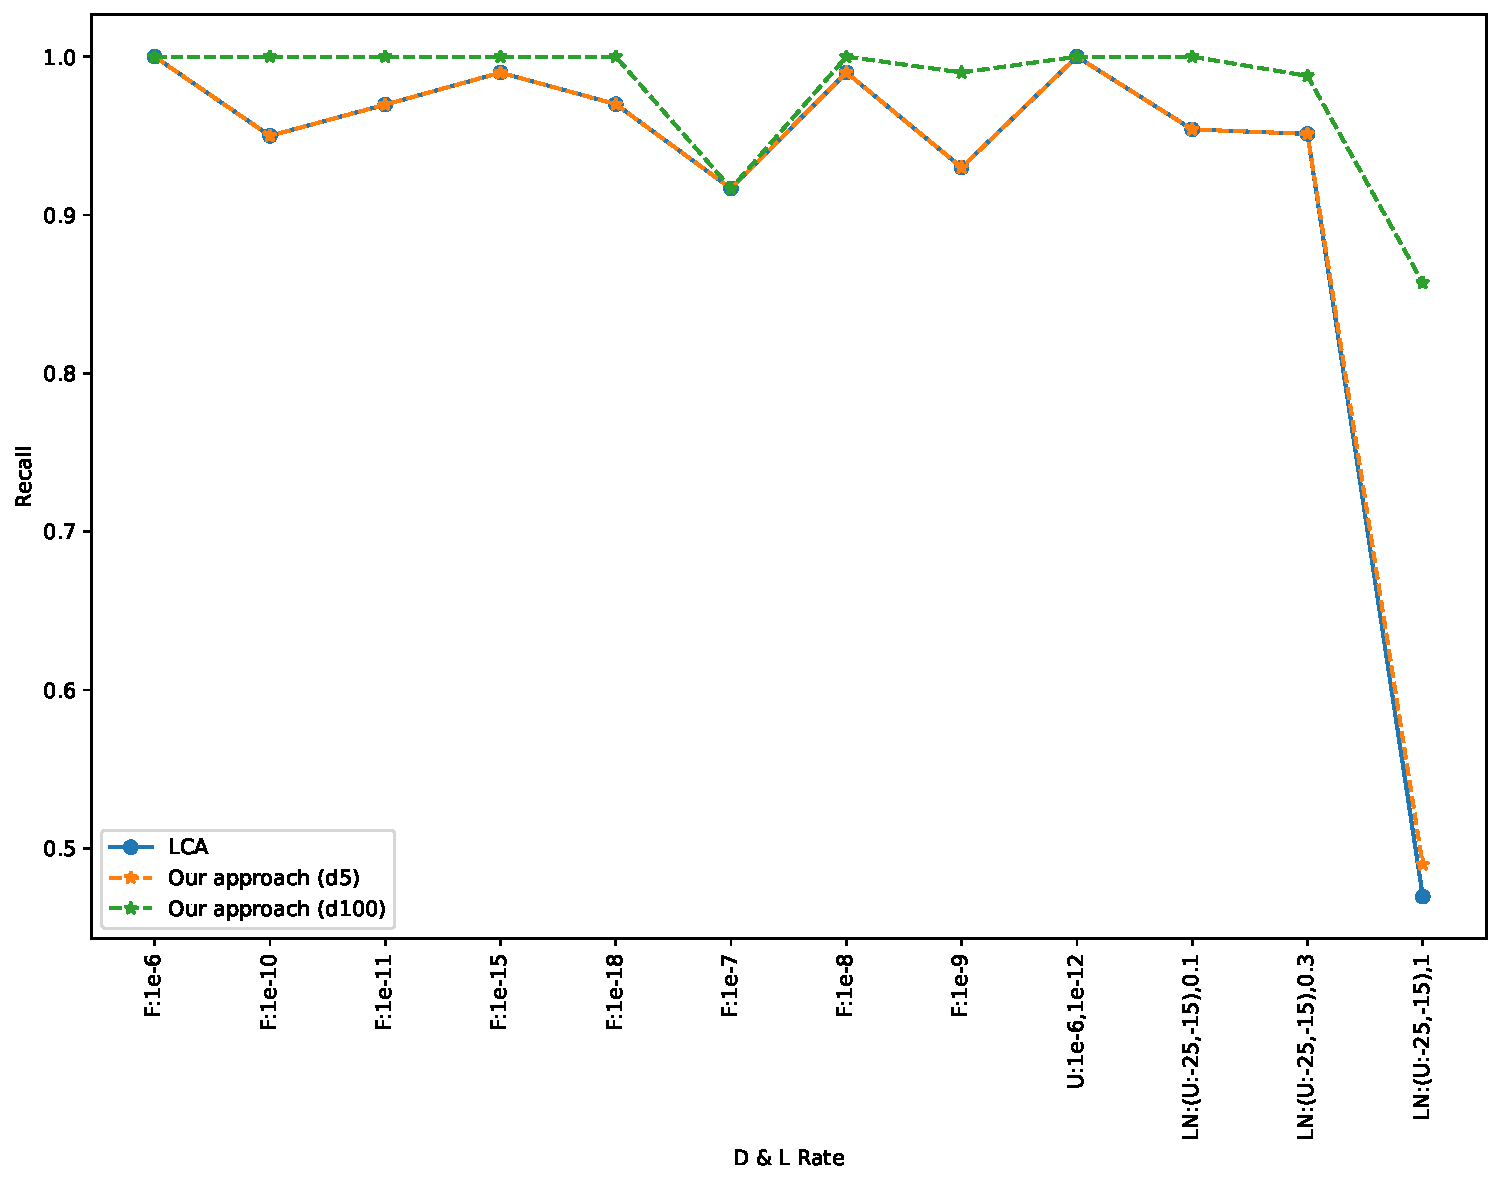
\includegraphics[width=\textwidth]{figs/recall-WGD-t10-t80-Avg.pdf}
        \caption{Recall of WGD for simulations with 1 WGD, averaged over 100 runs.}
        \label{fig:recall-wgd-1wgd}
    \end{subfigure}
    \hfill
    \begin{subfigure}[b]{0.48\textwidth}
        \centering
        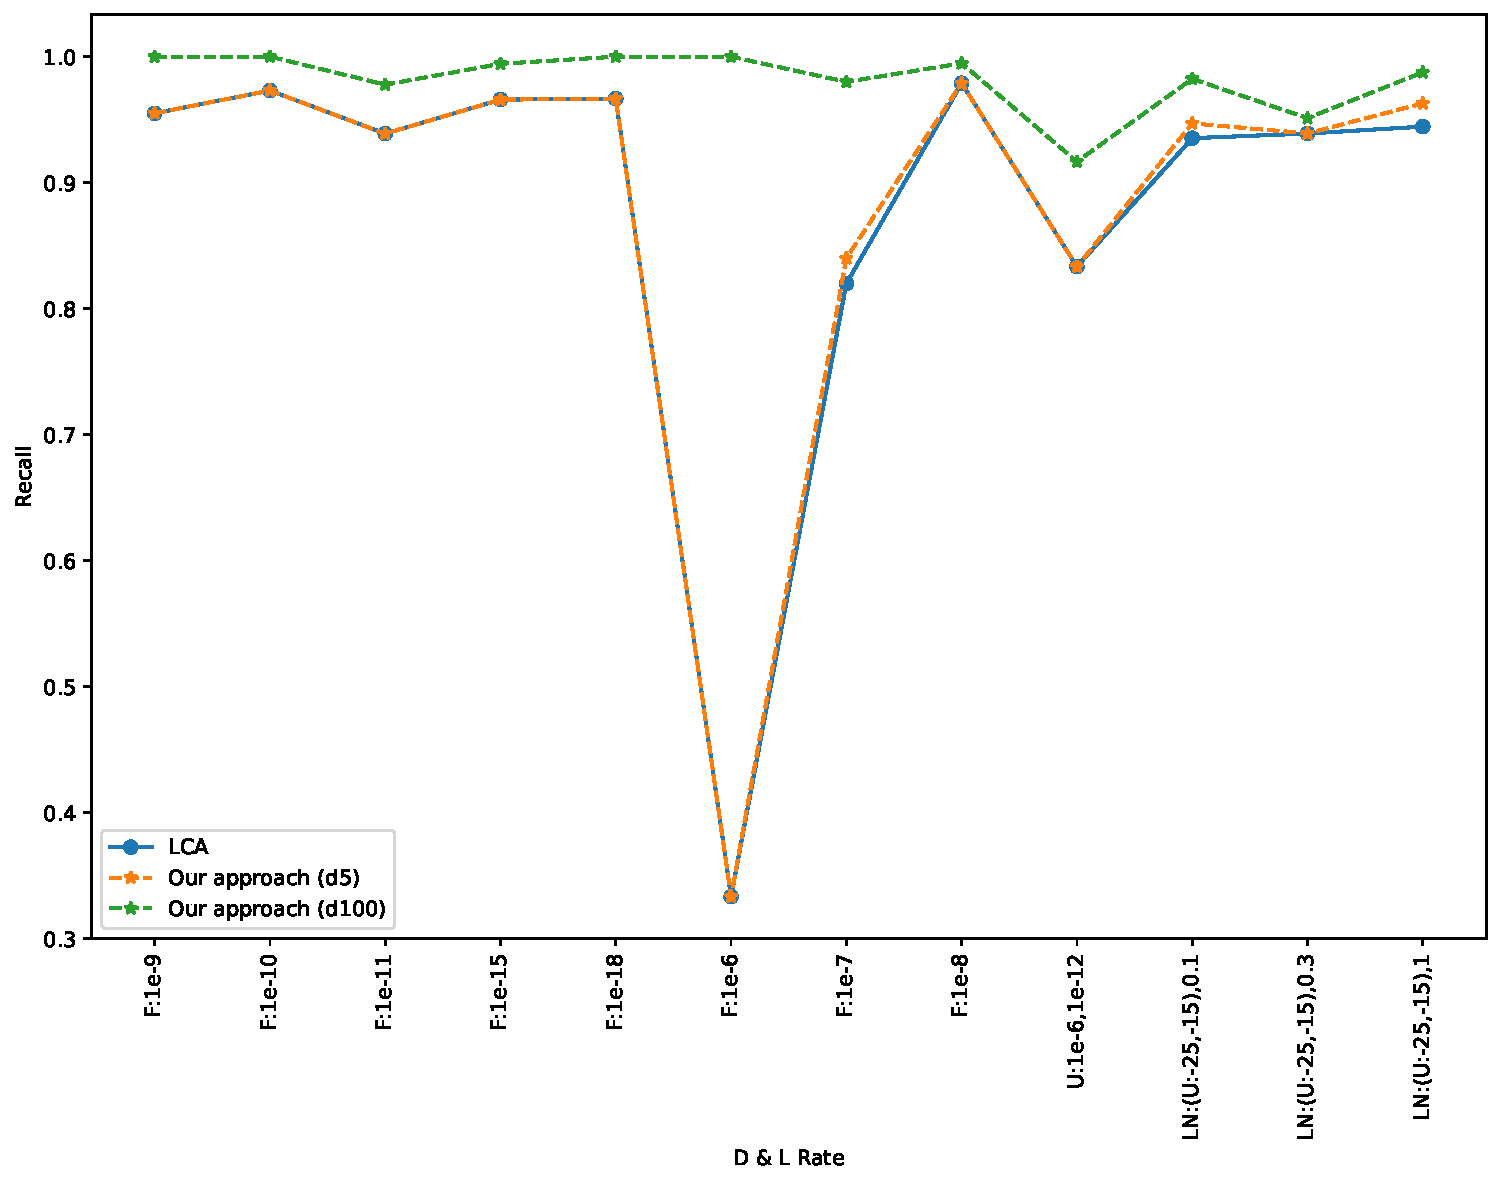
\includegraphics[width=\textwidth]{figs/recall-2W-WGD-t20-t80-Avg.pdf}
        \caption{Recall of WGD for simulations with 2 WGDs, averaged over 100 runs.}
        \label{fig:recall-wgd-2wgd}
    \end{subfigure}
    
    % Two subplots in the second row
    \begin{subfigure}[b]{0.48\textwidth}
        \centering
        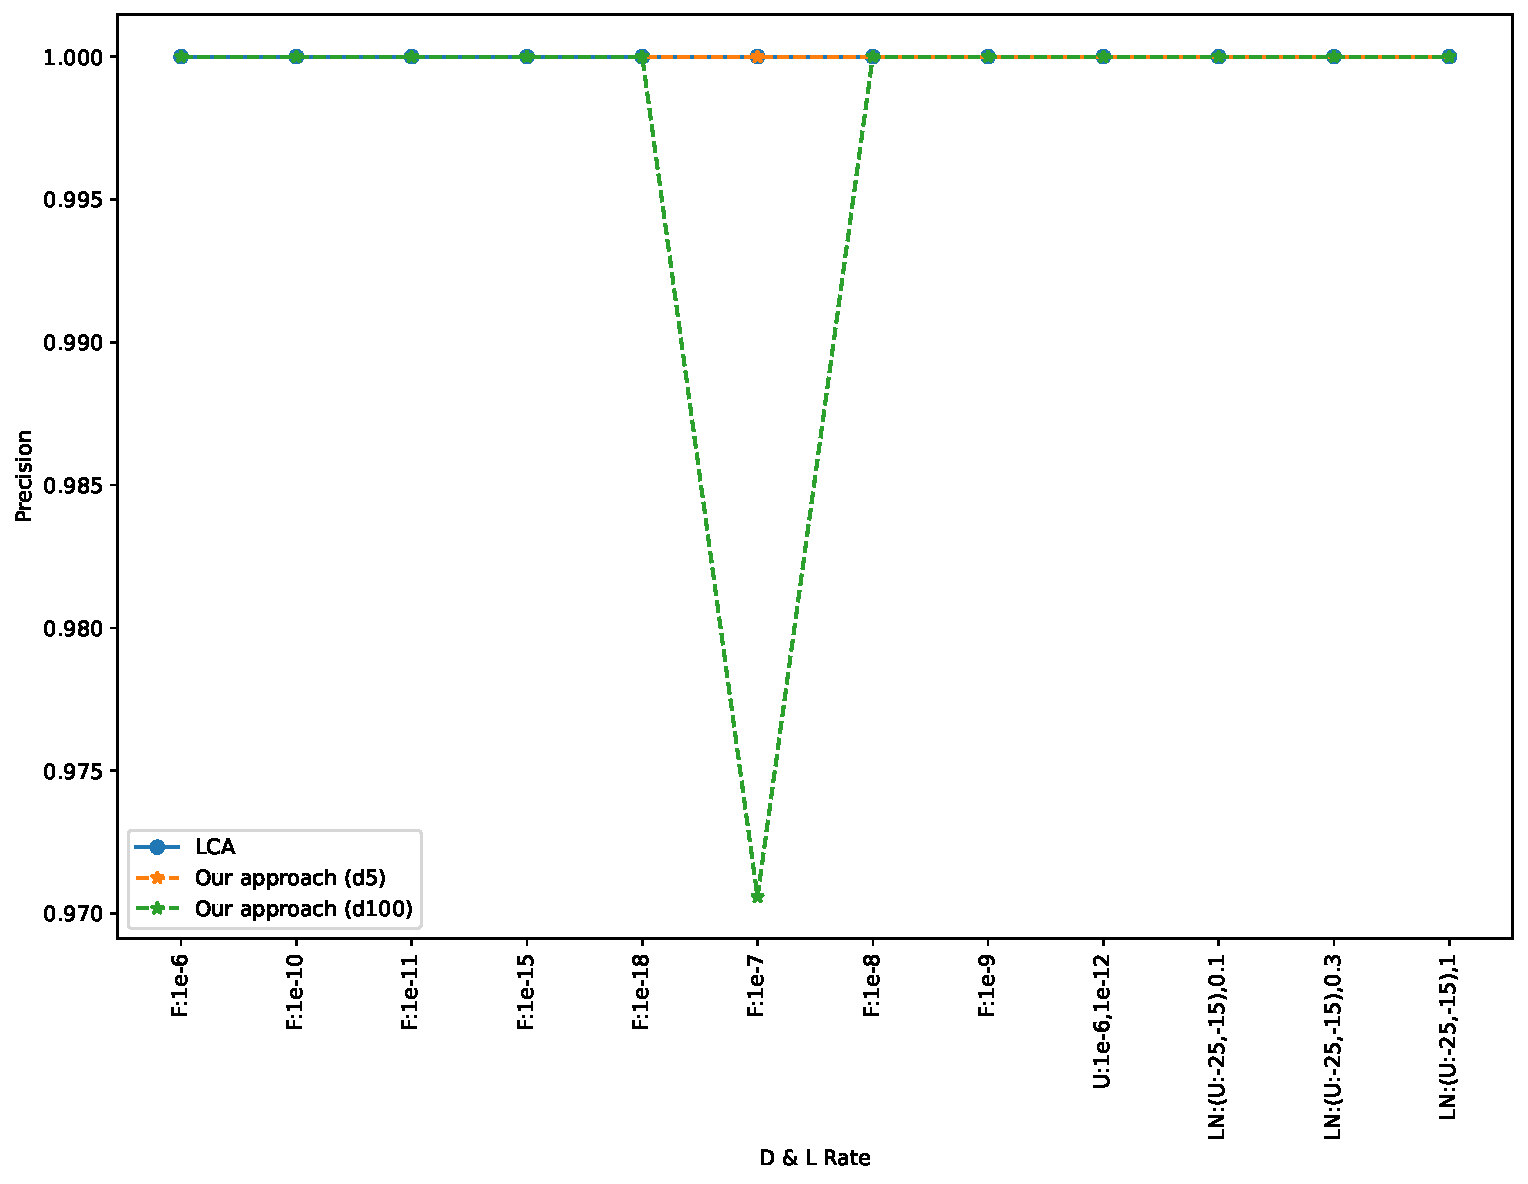
\includegraphics[width=\textwidth]{figs/precision-WGD-t10-t80-Avg.pdf}
        \caption{Precision of WGD for simulations with 1 WGD, averaged over 100 runs.}
        \label{fig:precision-wgd-1wgd}
    \end{subfigure}
    \hfill
    \begin{subfigure}[b]{0.48\textwidth}
        \centering
        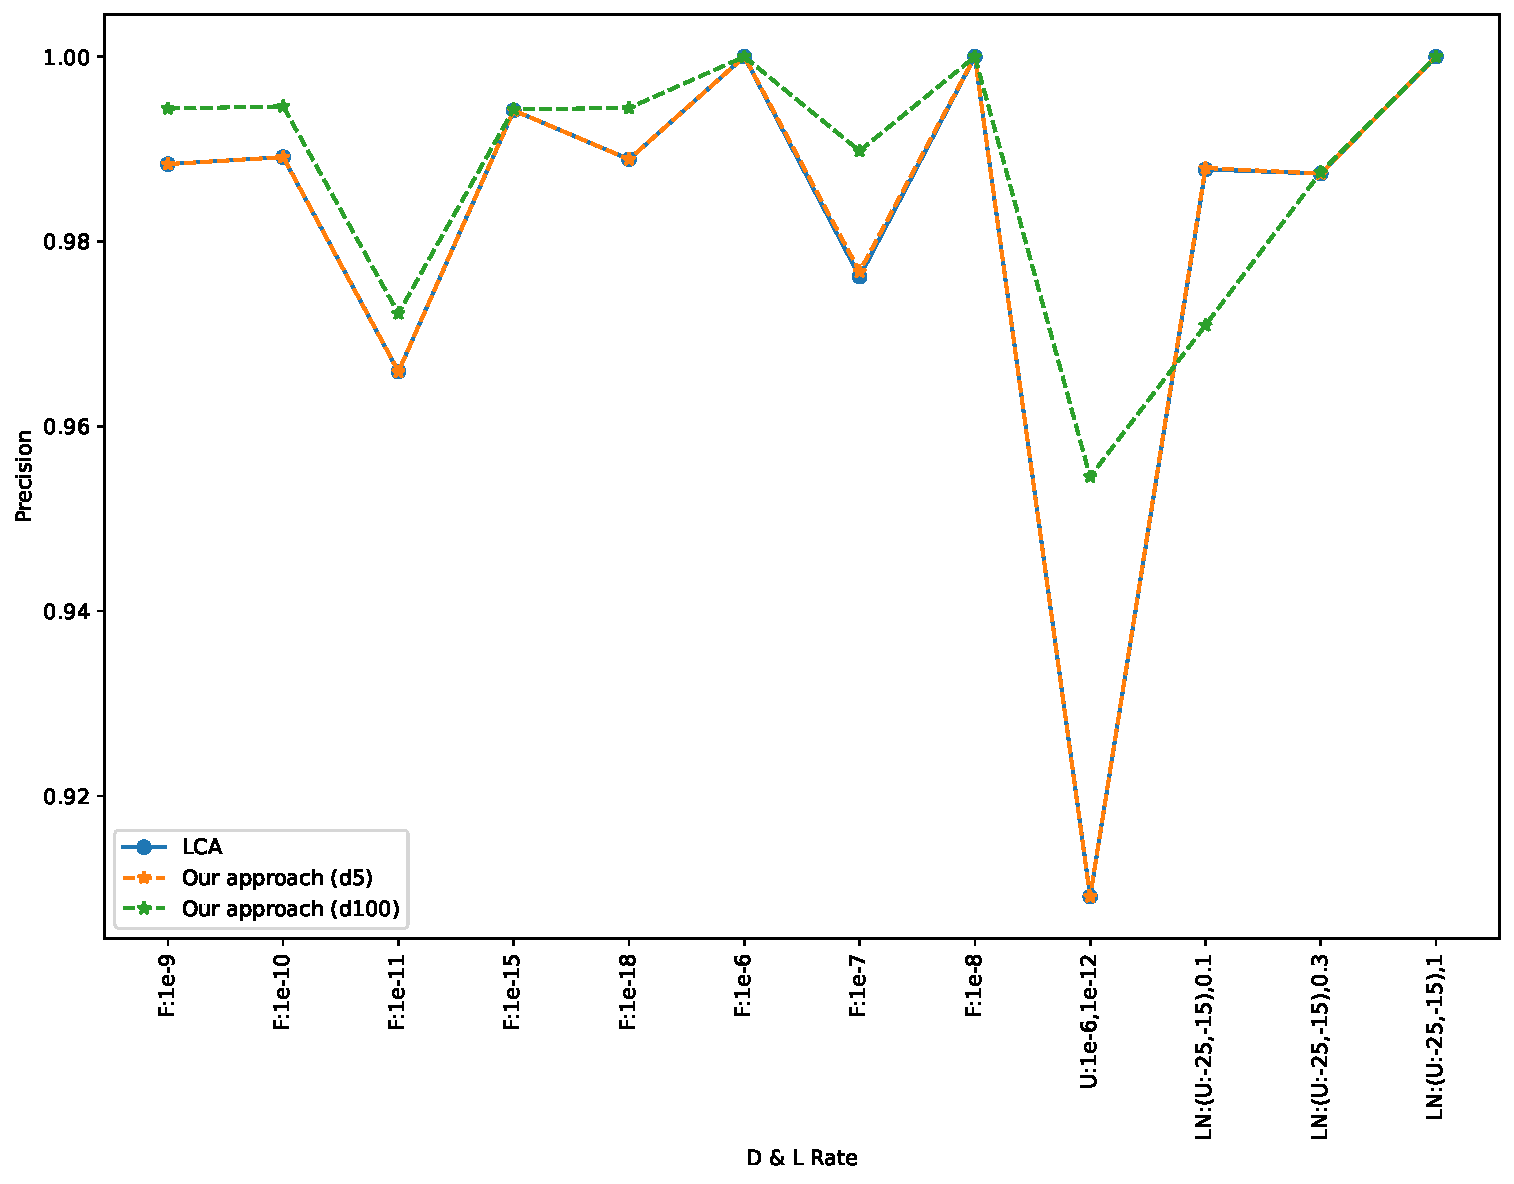
\includegraphics[width=\textwidth]{figs/precision-2W-WGD-t20-t80-Avg.pdf}
        \caption{Precision of WGD for simulations with 2 WGDs, averaged over 100 runs.}
        \label{fig:precision-wgd-2wgd}
    \end{subfigure}
    
    \caption{
Recall and Precision metrics for detecting Whole Genome Duplication (WGD) events in simulations containing either one or two WGDs, analyzed under varying duplication and loss rates. Each result is an average derived from 100 simulation runs, ensuring reliability and robustness of the findings. Subfigure (a) shows the Recall metric for simulations with a single WGD, while subfigure (b) presents the Recall for simulations with two WGDs. Subfigures (c) and (d) display the Precision metrics for simulations with one and two WGDs, respectively.
    }
    \label{fig:recall-precision-wgd}
\end{figure}





\begin{figure}[h!]
    \centering
    % First subplot at the top
    \begin{subfigure}[b]{0.48\textwidth}
        \centering
        \includegraphics[width=\textwidth]{figs/recall-sd-t20-t80-Avg.pdf}
        \caption{Recall of SD for simulations with 1 WGD, averaged over 100 runs.}
        \label{fig:recall-sd-1wgd}
    \end{subfigure}
    \hfill
    \begin{subfigure}[b]{0.48\textwidth}
        \centering
        \includegraphics[width=\textwidth]{figs/recall-2W-sd-t20-t80-Avg.pdf}
        \caption{Recall of SD for simulations with 2 WGDs, averaged over 100 runs.}
        \label{fig:recall-sd-2wgd}
    \end{subfigure}
    
    % Two subplots in the second row
    \begin{subfigure}[b]{0.48\textwidth}
        \centering
        \includegraphics[width=\textwidth]{figs/precision-sd-t20-t80-Avg.pdf}
        \caption{Precision of SD for simulations with 1 WGD, averaged over 100 runs.}
        \label{fig:precision-sd-1wgd}
    \end{subfigure}
    \hfill
    \begin{subfigure}[b]{0.48\textwidth}
        \centering
        \includegraphics[width=\textwidth]{figs/precision-2W-sd-t20-t80-Avg.pdf}
        \caption{Precision of SD for simulations with 2 WGDs, averaged over 100 runs.}
        \label{fig:precision-sd-2wgd}
    \end{subfigure}
    
    \caption{
        Recall and Precision metrics for predicting Segmental Duplications (SDs) in simulations featuring either one or two Whole Genome Duplications (WGDs), evaluated under different duplication and loss rates. Each metric is averaged over 100 simulation runs to ensure robust statistical significance. Subfigures (a) and (b) display the Recall for simulations with 1 and 2 WGDs, respectively, while subfigures (c) and (d) present the corresponding Precision metrics. These plots provide insights into the algorithm's ability to accurately predict SDs under varying evolutionary scenarios.
    }
    \label{fig:recall-precision-sd}
\end{figure}


\subsection{Results under Nearest Neighbor Interchanges (NNI) Event}

In this section, we analyze the performance of our approach when Nearest Neighbor Interchanges (NNI) events are introduced into the gene trees. NNI is a tree rearrangement method that swaps the subtrees around an internal node, effectively altering the tree topology without changing the leaf labels. By applying NNIs, we simulate more complex evolutionary scenarios that challenge the accuracy of ancestral mapping.

We conducted a series of experiments where NNI events were applied to the gene trees after simulating duplications and losses with SimPhy. These tests allow us to evaluate the robustness of our algorithm in dealing with uncertainties introduced by such topological changes. Specifically, we analyze how the introduction of NNI events impacts the recall and precision metrics for WGDs and SDs in both one and two WGD simulations.

We define a value $k$ in NNI, representing the number of Nearest Neighbor Interchanges applied to each gene tree. To assess the impact of varying degrees of tree rearrangement, we tested three different values of $k$: a low NNI rate ($k=1$), a medium NNI rate ($k=5$), and a high NNI rate ($k=15$). These values correspond to increasing levels of topological alteration in the gene trees, simulating various degrees of evolutionary complexity.

In Figures \ref{fig:recall-precision-wgd-NNI} and \ref{fig:recall-precision-2wgd-NNI}, we present the recall and precision metrics for simulations containing one and two WGDs, respectively. In terms of recall, we observe that across all NNI rates, our approach consistently outperforms the LCA method, particularly when two WGD events are present. This suggests that even under significant gene tree rearrangements, our method is better at recovering true WGD events compared to the LCA-based mapping.

However, in terms of precision, we note that for scenarios with high duplication and loss rates, our approach exhibits a lower precision rate, particularly as the NNI rate increases. This indicates that, while our method successfully identifies many true positives, it also introduces more false positives under high NNI and complex duplication scenarios. This trend is more pronounced in simulations with higher duplication rates and complex topological rearrangements, where over-estimating WGD events may become an issue.

These results highlight the robustness of our approach in recovering WGD events under varying levels of tree rearrangement, while also pointing out potential areas for improvement in precision, particularly under high duplication rates and extensive tree modifications.



\begin{figure}[h!]
    \centering
    % First row of three subplots
    \begin{subfigure}[b]{0.31\textwidth}
        \centering
        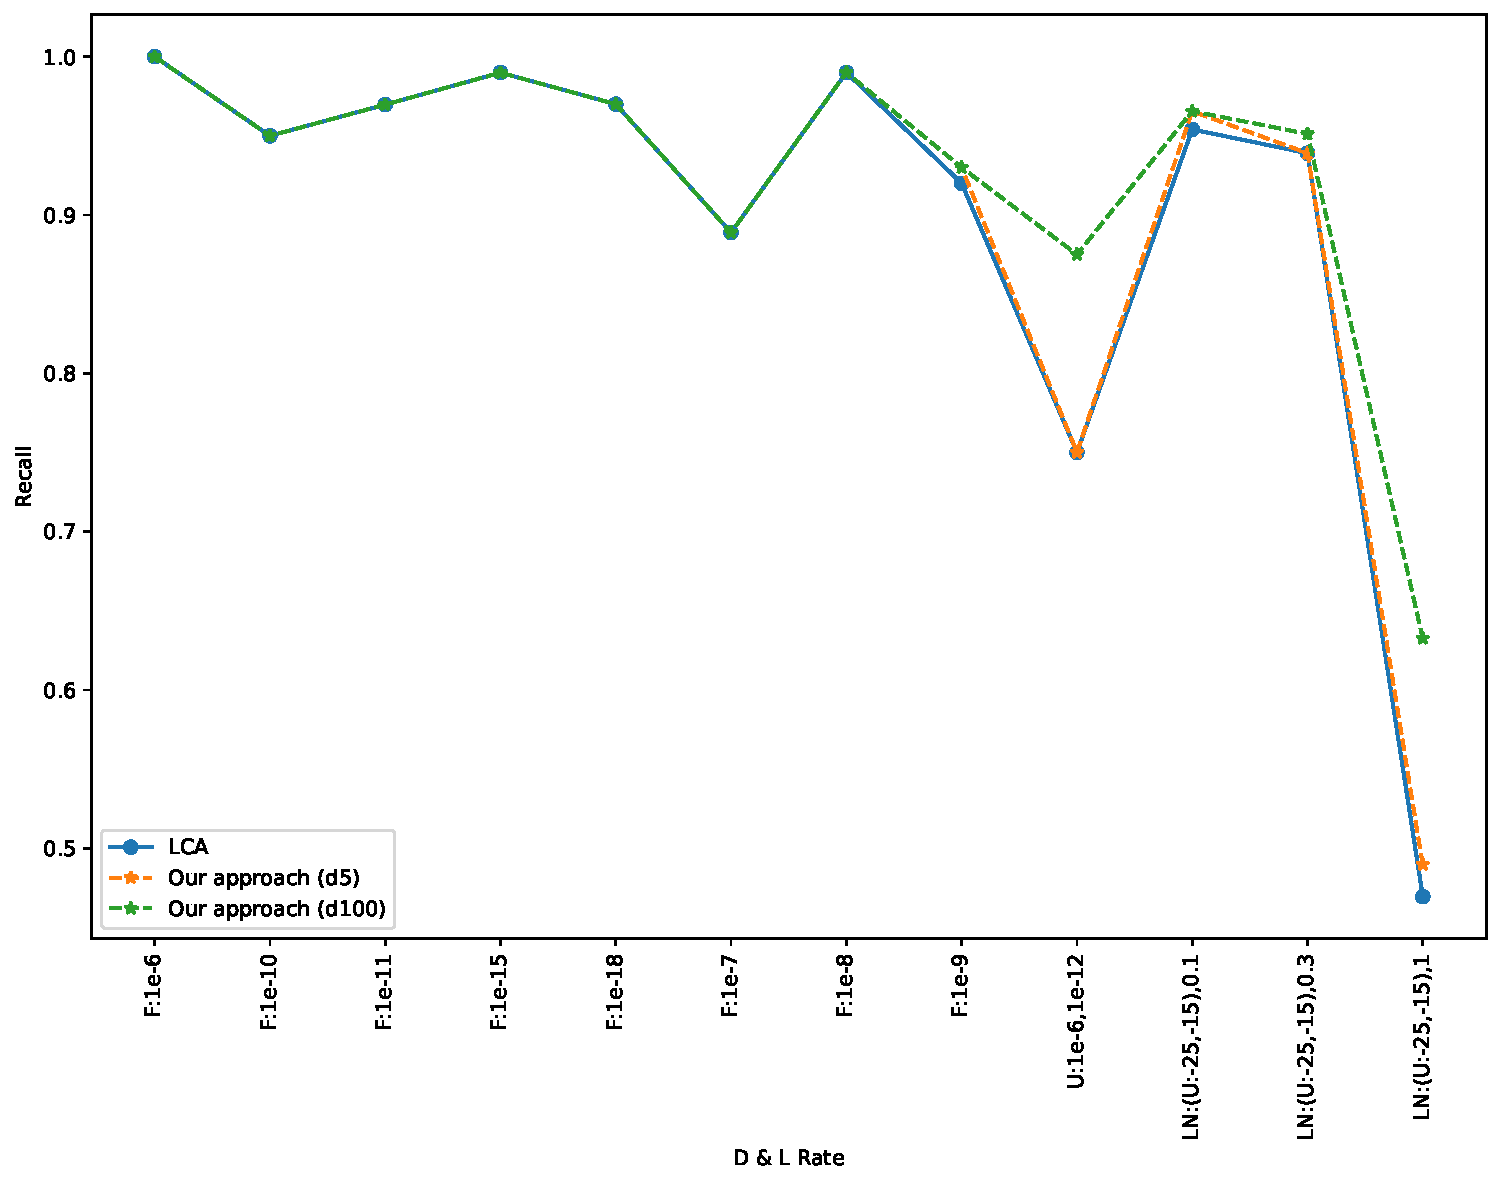
\includegraphics[width=\textwidth]{figs/recall-NNI-K1-WGD-t20-t80-Avg.pdf}
        \caption{Recall of WGDs for simulations with 1 WGD under NNI when k=1, averaged over 100 runs.}
        \label{fig:recall-NNI-k1-wgd}
    \end{subfigure}
    \hfill
    \begin{subfigure}[b]{0.31\textwidth}
        \centering
        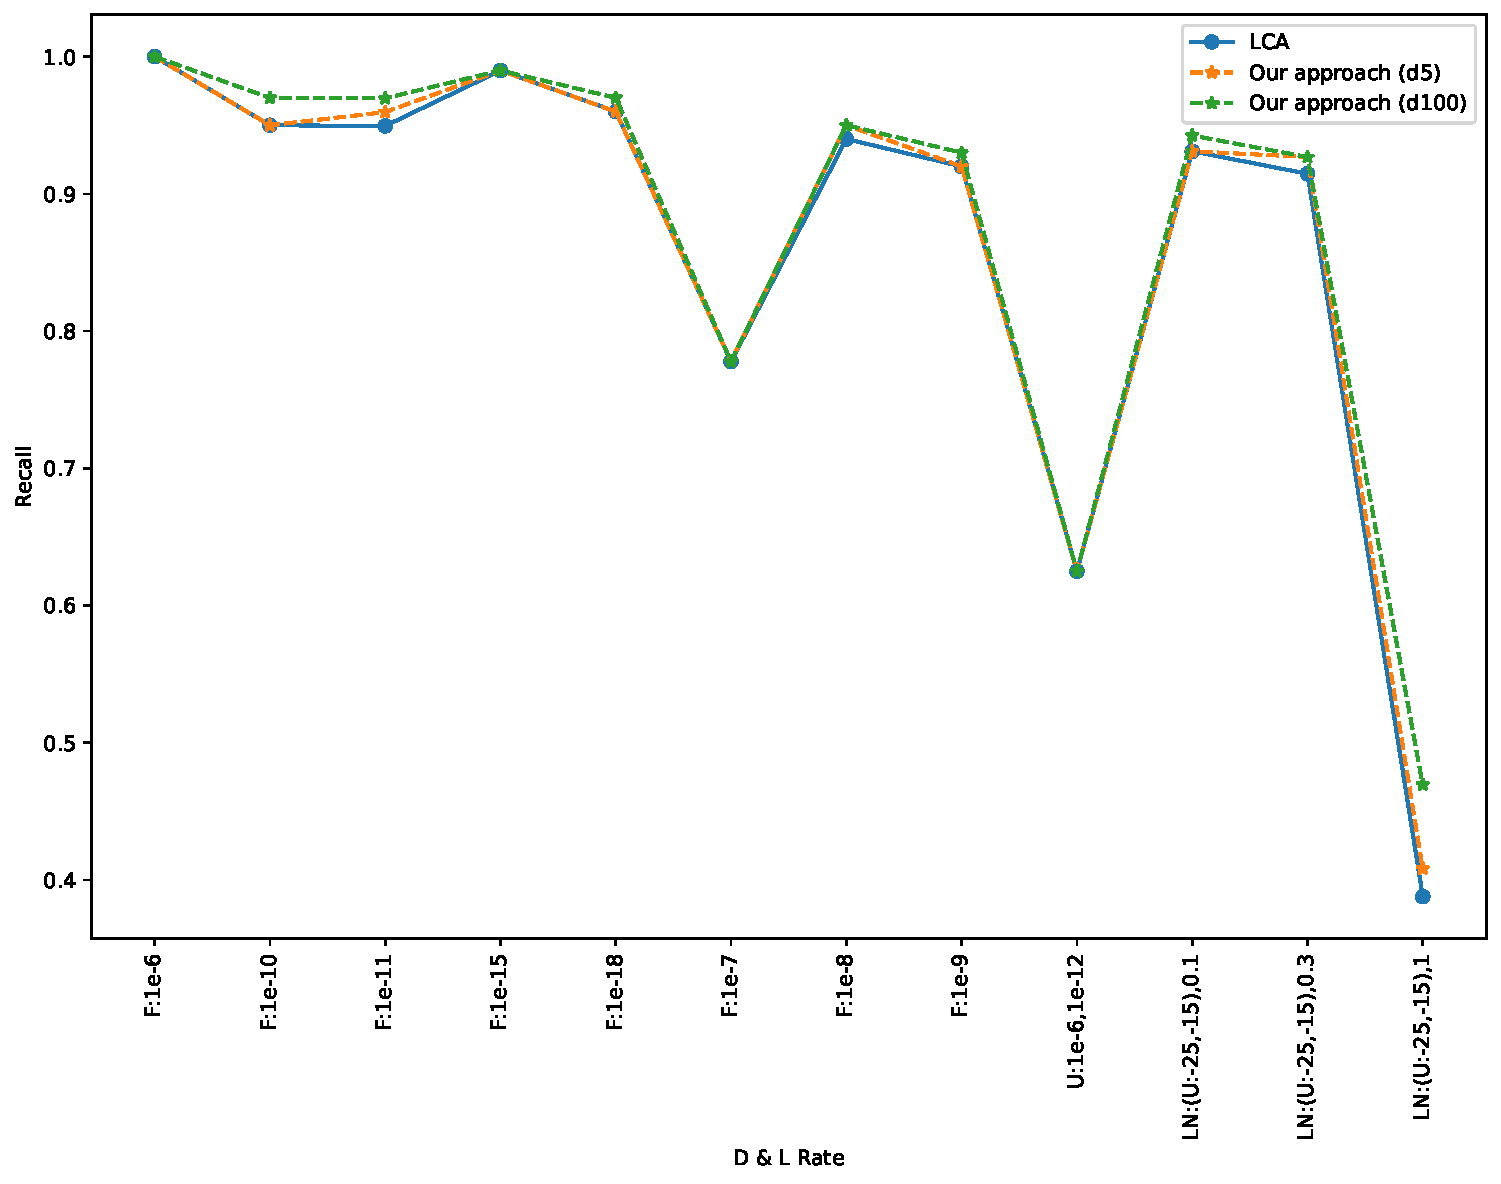
\includegraphics[width=\textwidth]{figs/recall-NNI-K5-WGD-t20-t80-Avg.pdf}
        \caption{Recall of WGDs for simulations with 1 WGD under NNI when k=5, averaged over 100 runs.}
        \label{fig:recall-NNI-k5-wgd}
    \end{subfigure}
    \hfill
    \begin{subfigure}[b]{0.31\textwidth}
        \centering
        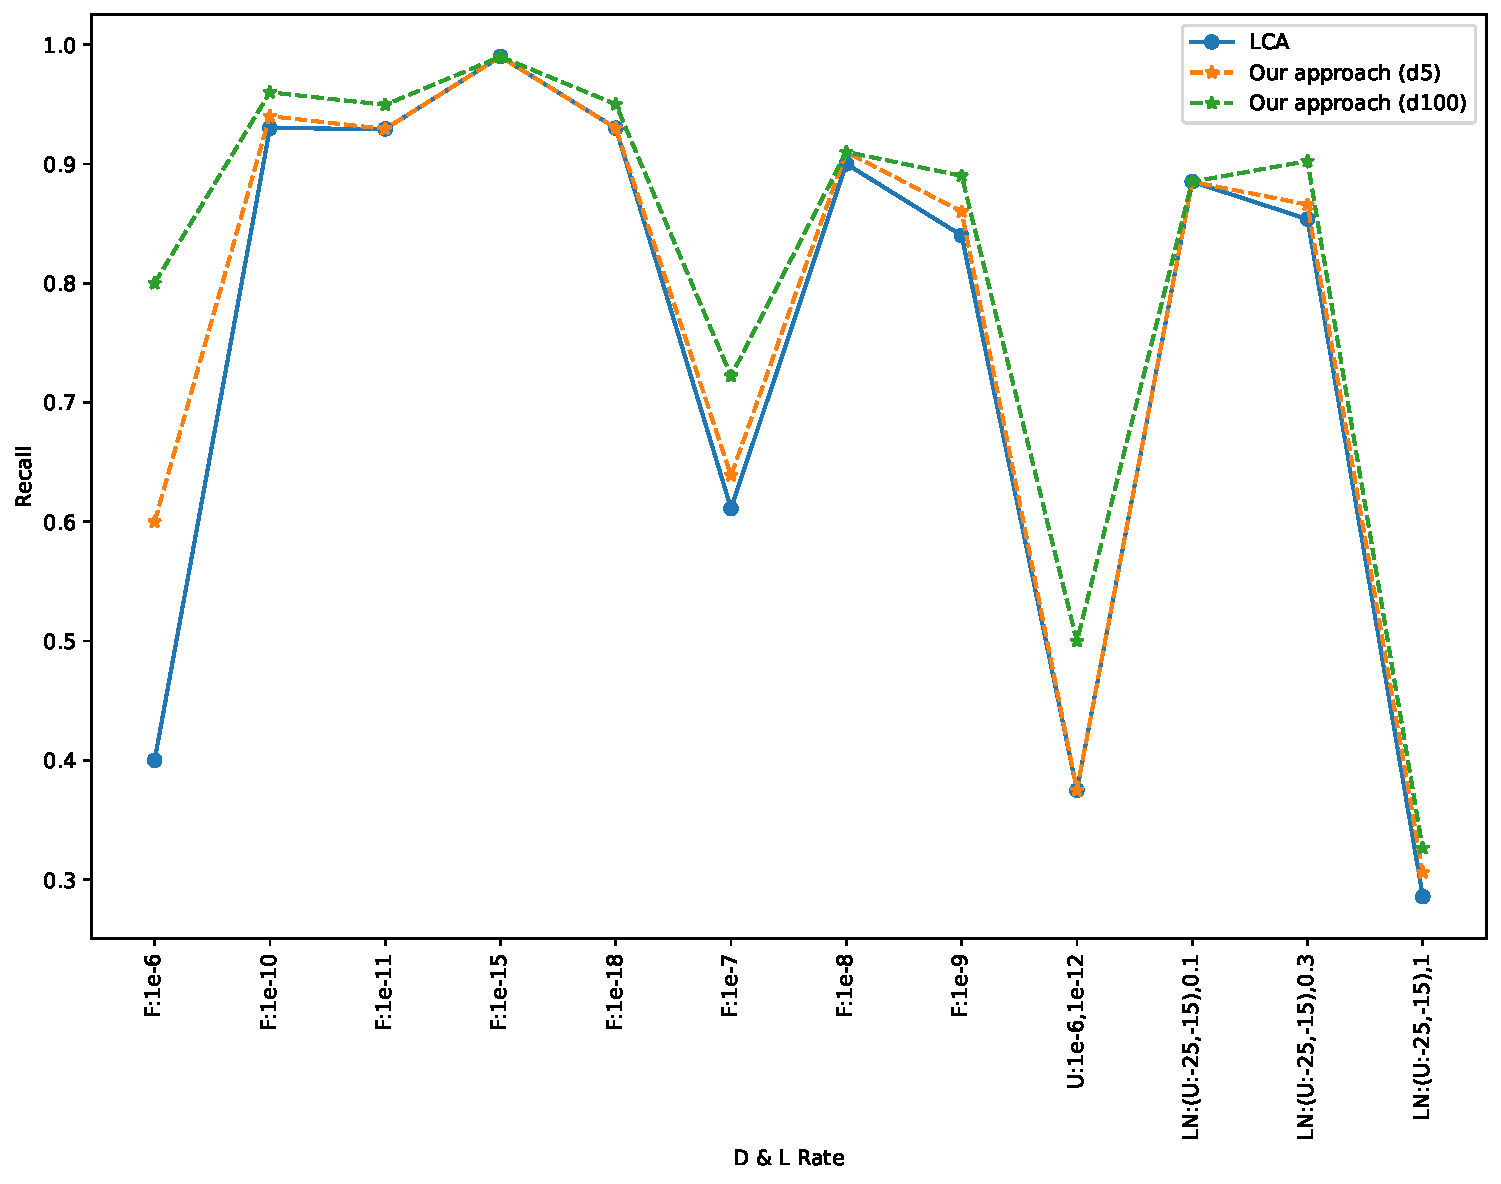
\includegraphics[width=\textwidth]{figs/recall-NNI-K15-WGD-t20-t80-Avg.pdf}
        \caption{Recall of WGDs for simulations with 1 WGD under NNI when k=15, averaged over 100 runs.}
        \label{fig:recall-NNI-k15-wgd}
    \end{subfigure}
    
    \vspace{1em} % Adds space between the two rows

    % Second row of three subplots
    \begin{subfigure}[b]{0.31\textwidth}
        \centering
        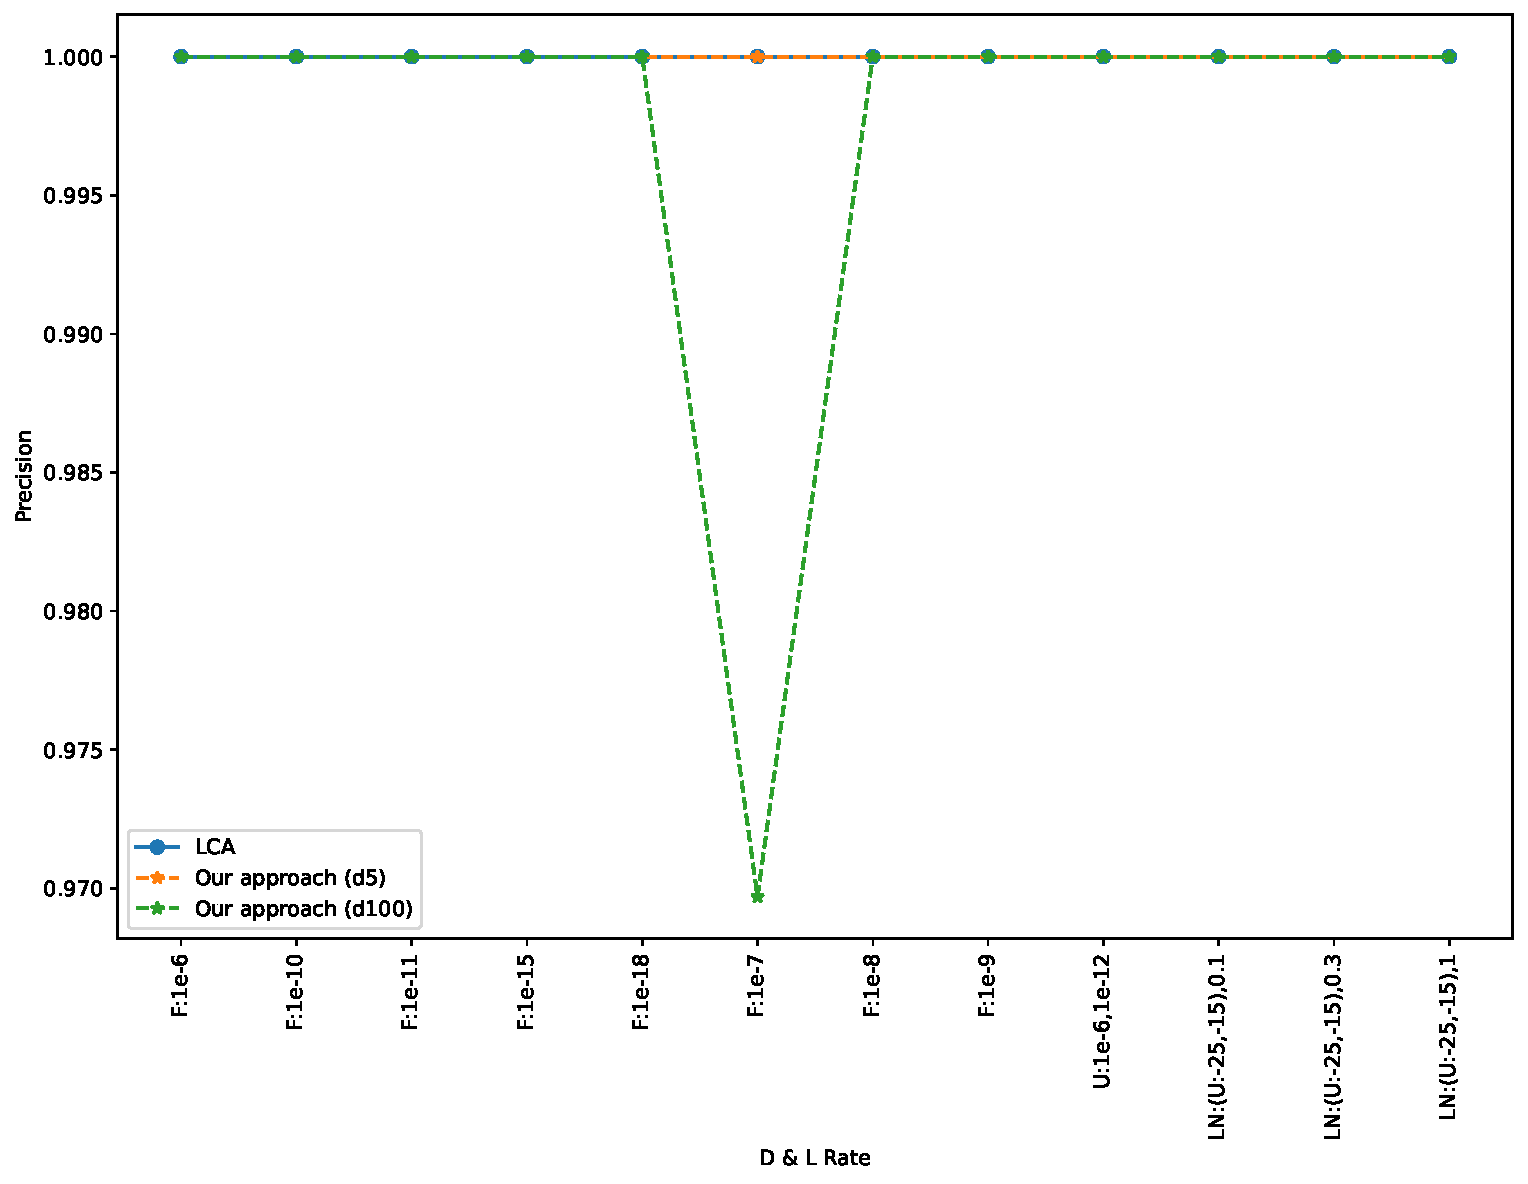
\includegraphics[width=\textwidth]{figs/precision-NNI-K1-WGD-t20-t80-Avg.pdf}
        \caption{Precision of WGDs for simulations with 1 WGD under NNI when k=1, averaged over 100 runs.}
        \label{fig:precision-NNI-k1-wgd}
    \end{subfigure}
    \hfill
    \begin{subfigure}[b]{0.31\textwidth}
        \centering
        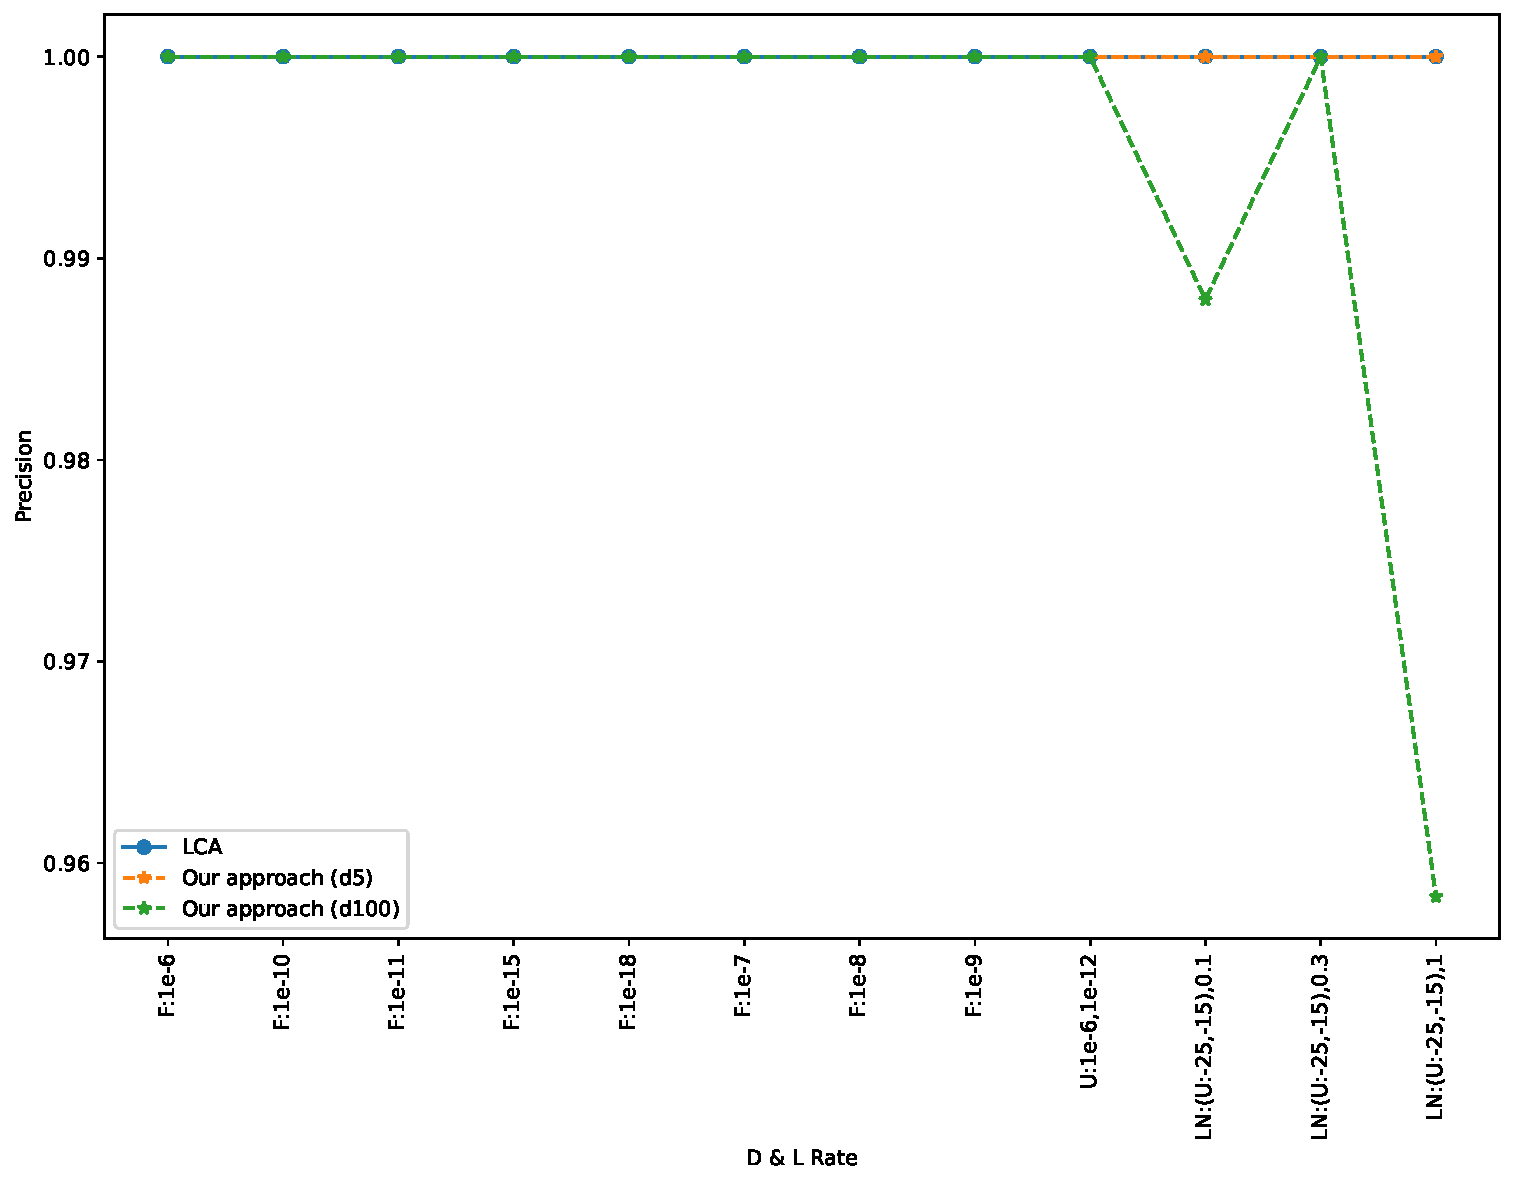
\includegraphics[width=\textwidth]{figs/precision-NNI-K5-WGD-t20-t80-Avg.pdf}
        \caption{Precision of WGDs for simulations with 1 WGD under NNI when k=5, averaged over 100 runs.}
        \label{fig:precision-NNI-k5-wgd}
    \end{subfigure}
    \hfill
    \begin{subfigure}[b]{0.31\textwidth}
        \centering
        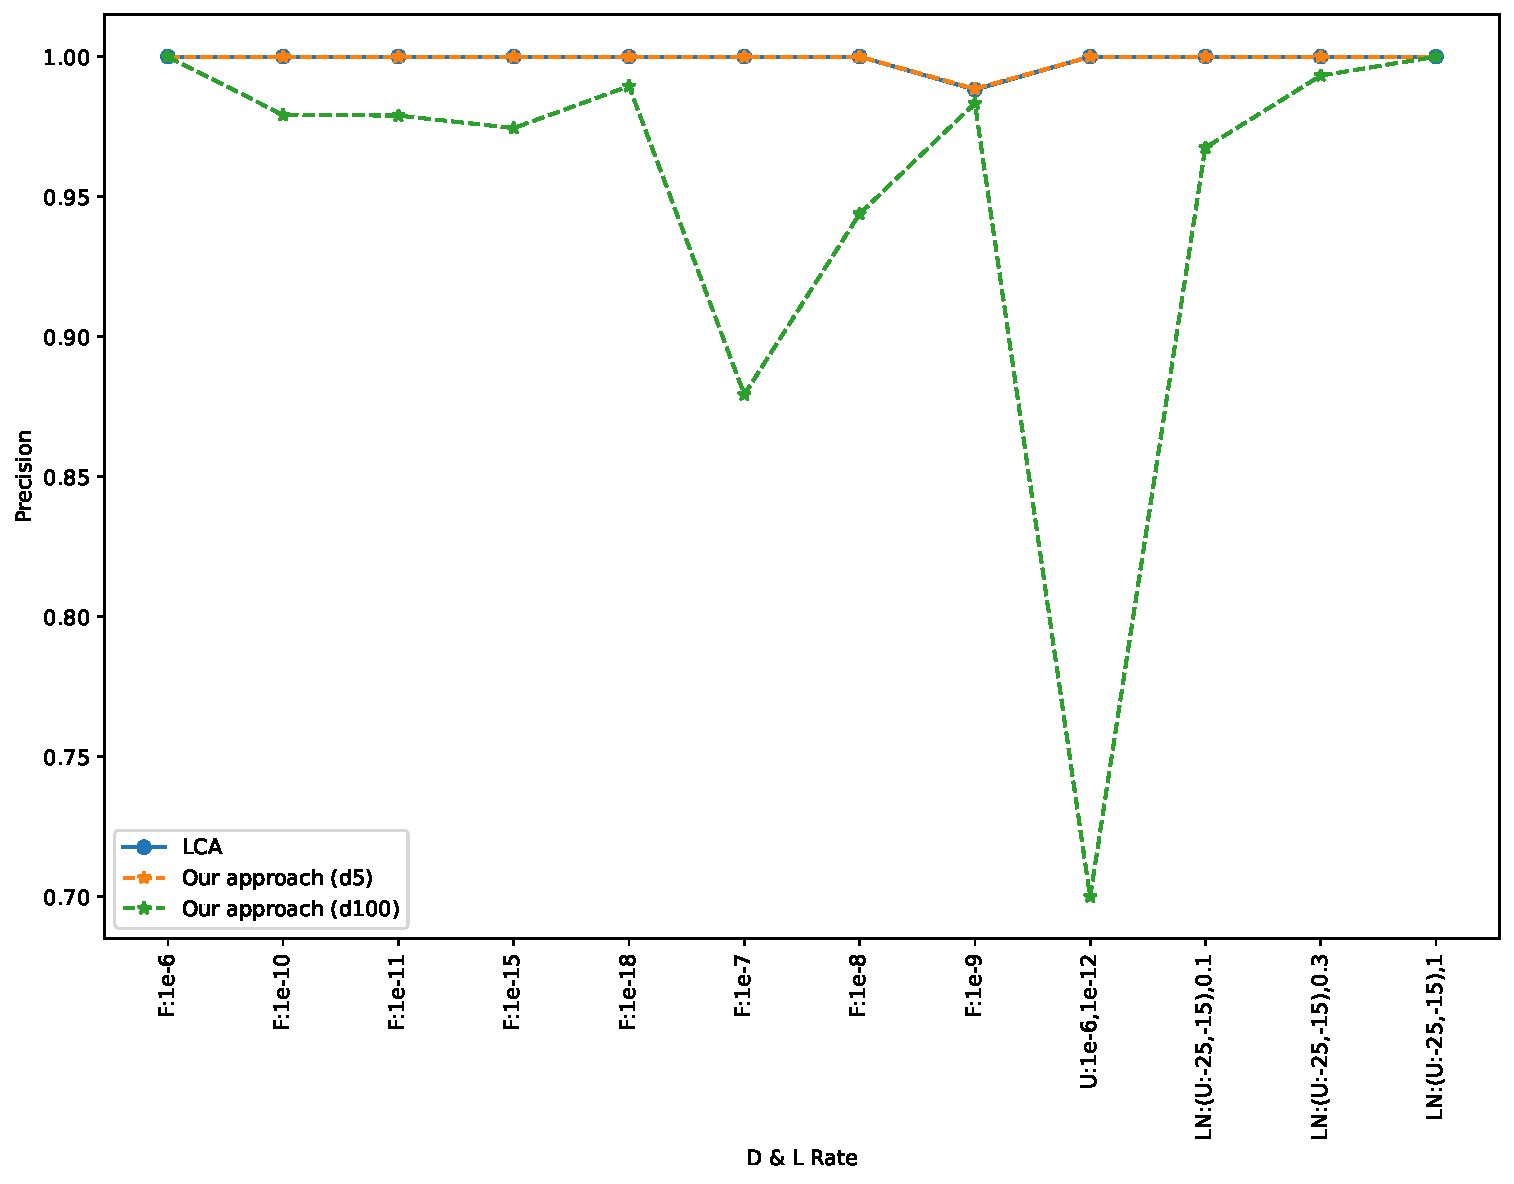
\includegraphics[width=\textwidth]{figs/precision-NNI-K15-WGD-t20-t80-Avg.pdf}
        \caption{Precision of WGDs for simulations with 1 WGD under NNI when k=15, averaged over 100 runs.}
        \label{fig:precision-NNI-k15-wgd}
    \end{subfigure}
    
    \caption{
        Comparison of Recall and Precision metrics for predicting Whole Genome Duplications (WGDs) in simulations with 1 WGD under Nearest Neighbor Interchanges (NNI) events. The parameter $k$ represents the number of NNIs applied to each gene tree. The simulations span varying duplication and loss rates and are averaged over 100 runs. Subfigures (a), (b), and (c) show Recall metrics for $k=1$, $k=5$, and $k=15$ NNIs, respectively. Subfigures (d), (e), and (f) present the corresponding Precision metrics under the same conditions.
    }
    \label{fig:recall-precision-wgd-NNI}
\end{figure}


\begin{figure}[h!]
    \centering
    % First row of three subplots
    \begin{subfigure}[b]{0.31\textwidth}
        \centering
        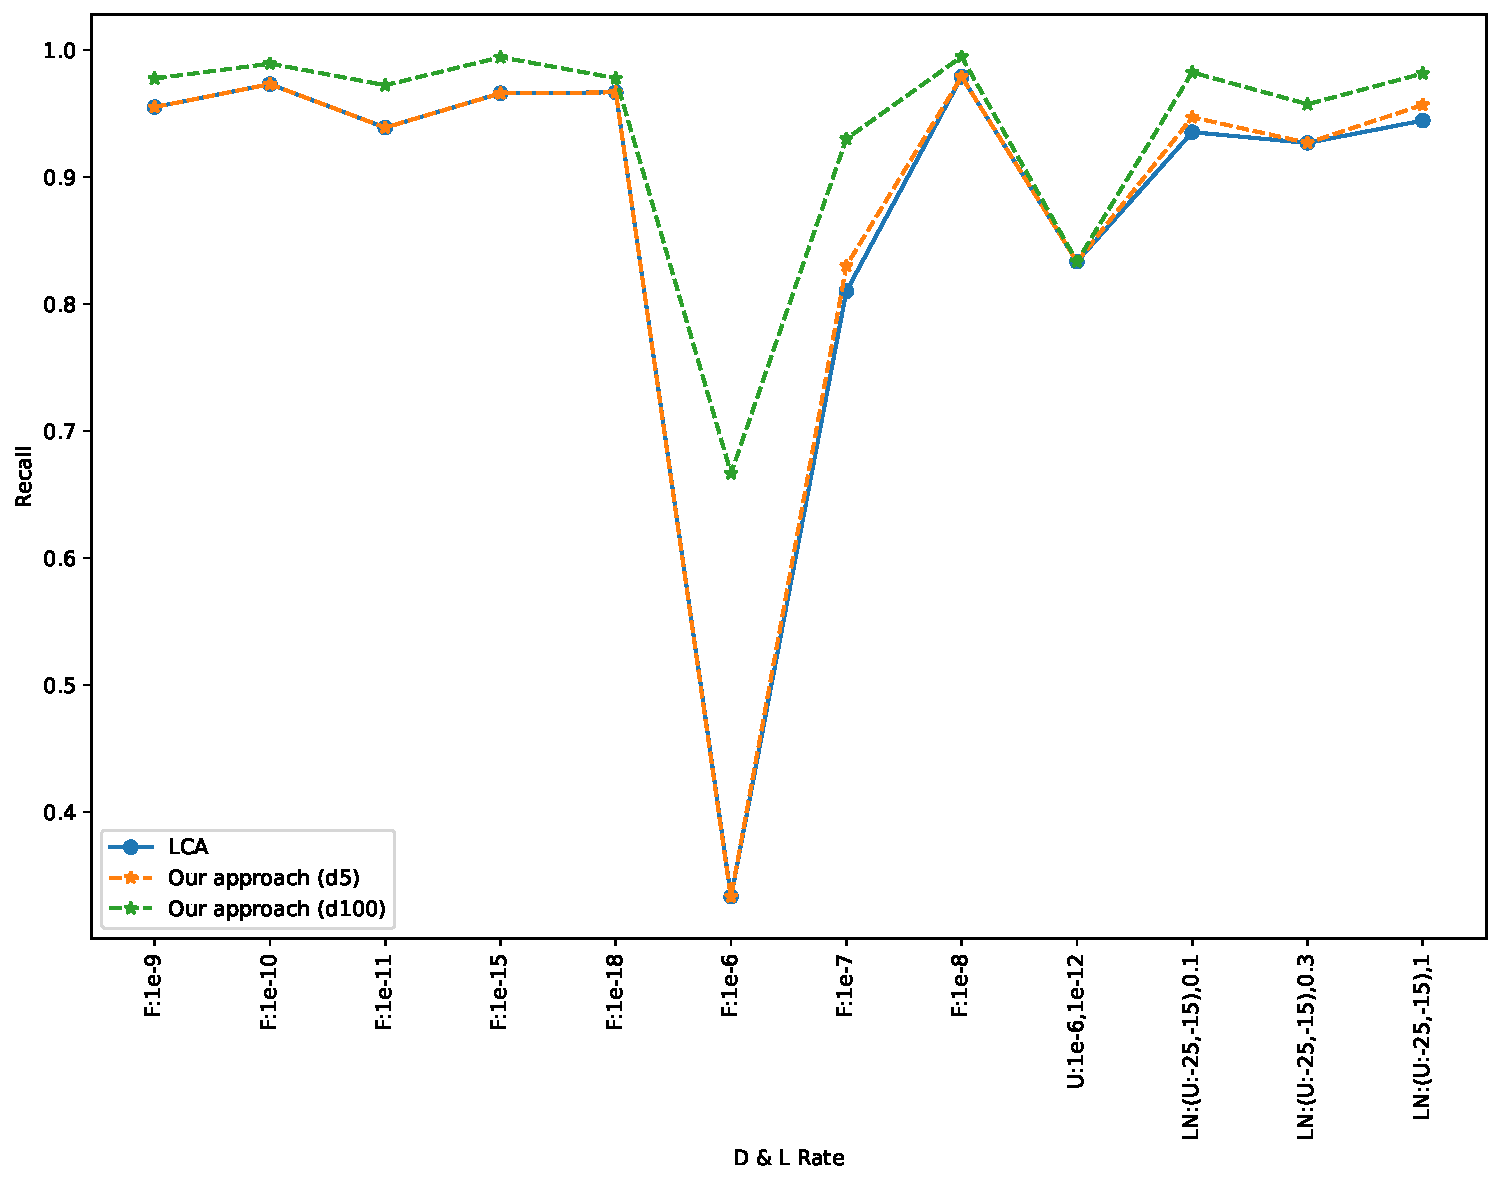
\includegraphics[width=\textwidth]{figs/recall-2W-NNI-K1-WGD-t20-t80-Avg.pdf}
        \caption{Recall of WGDs for simulations with 2 WGD under NNI when k=1, averaged over 100 runs.}
        \label{fig:recall-NNI-k1-2wgd}
    \end{subfigure}
    \hfill
    \begin{subfigure}[b]{0.31\textwidth}
        \centering
        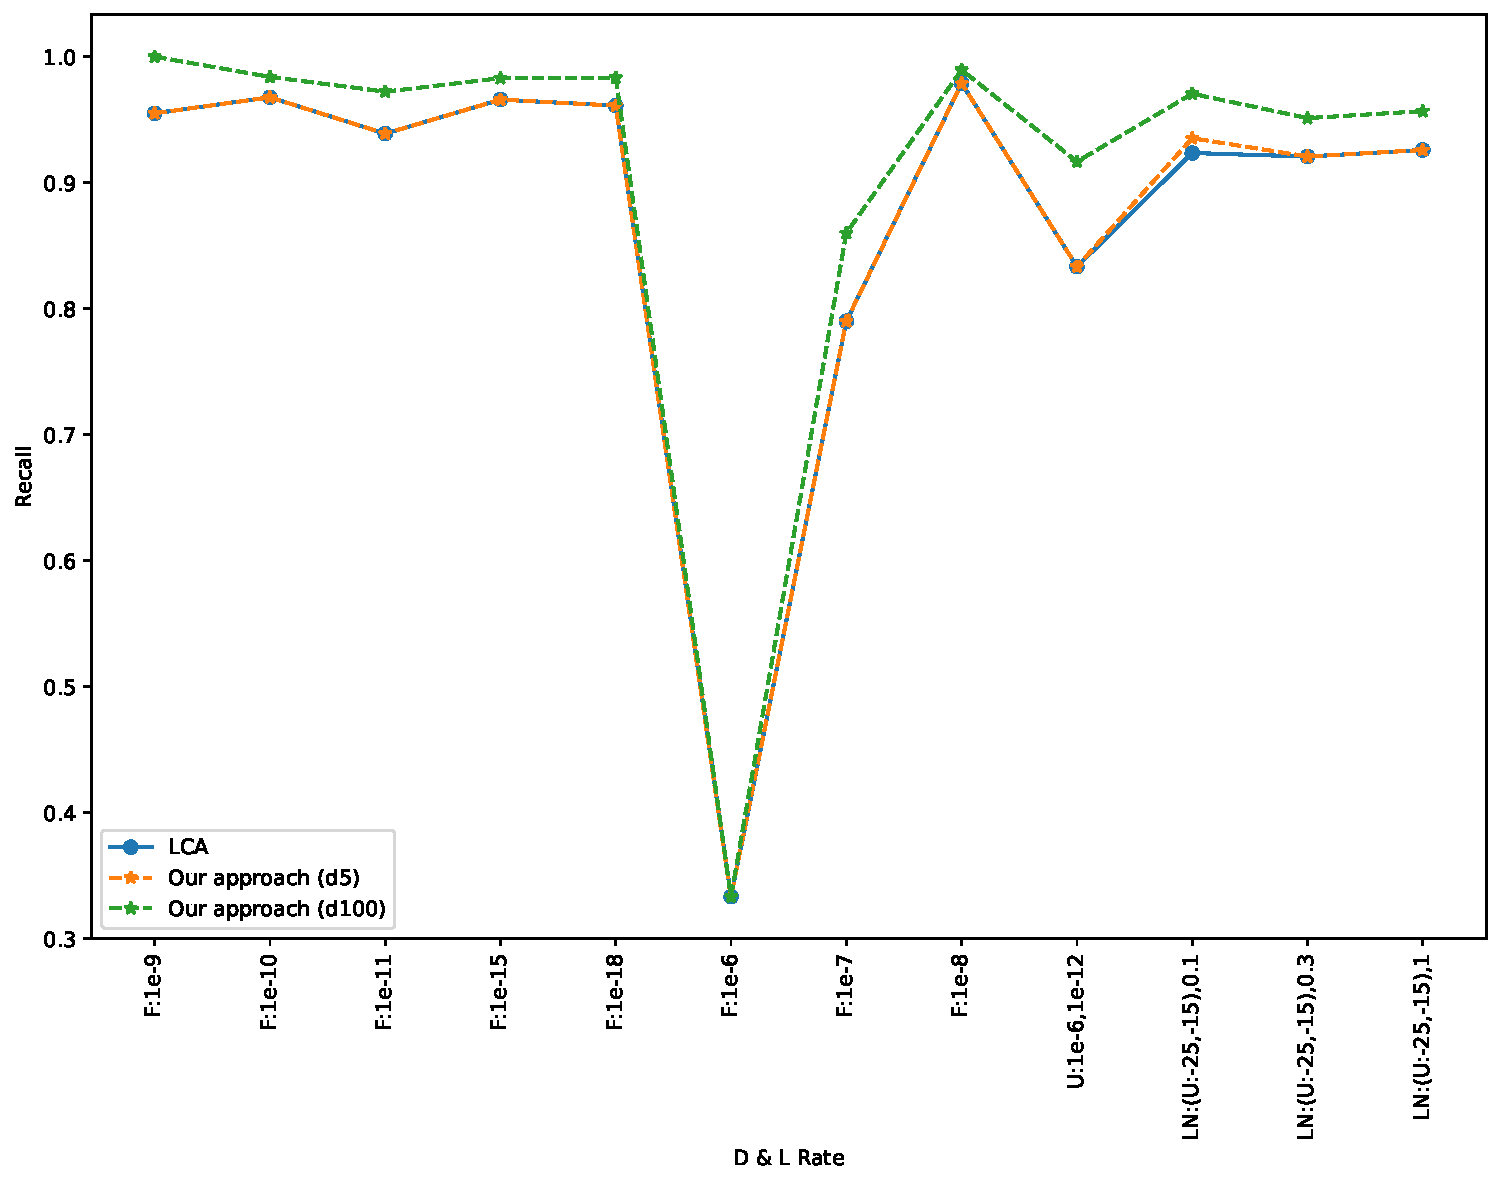
\includegraphics[width=\textwidth]{figs/recall-2W-NNI-K5-WGD-t20-t80-Avg.pdf}
        \caption{Recall of WGDs for simulations with 2 WGD under NNI when k=5, averaged over 100 runs.}
        \label{fig:recall-NNI-k5-2wgd}
    \end{subfigure}
    \hfill
    \begin{subfigure}[b]{0.31\textwidth}
        \centering
        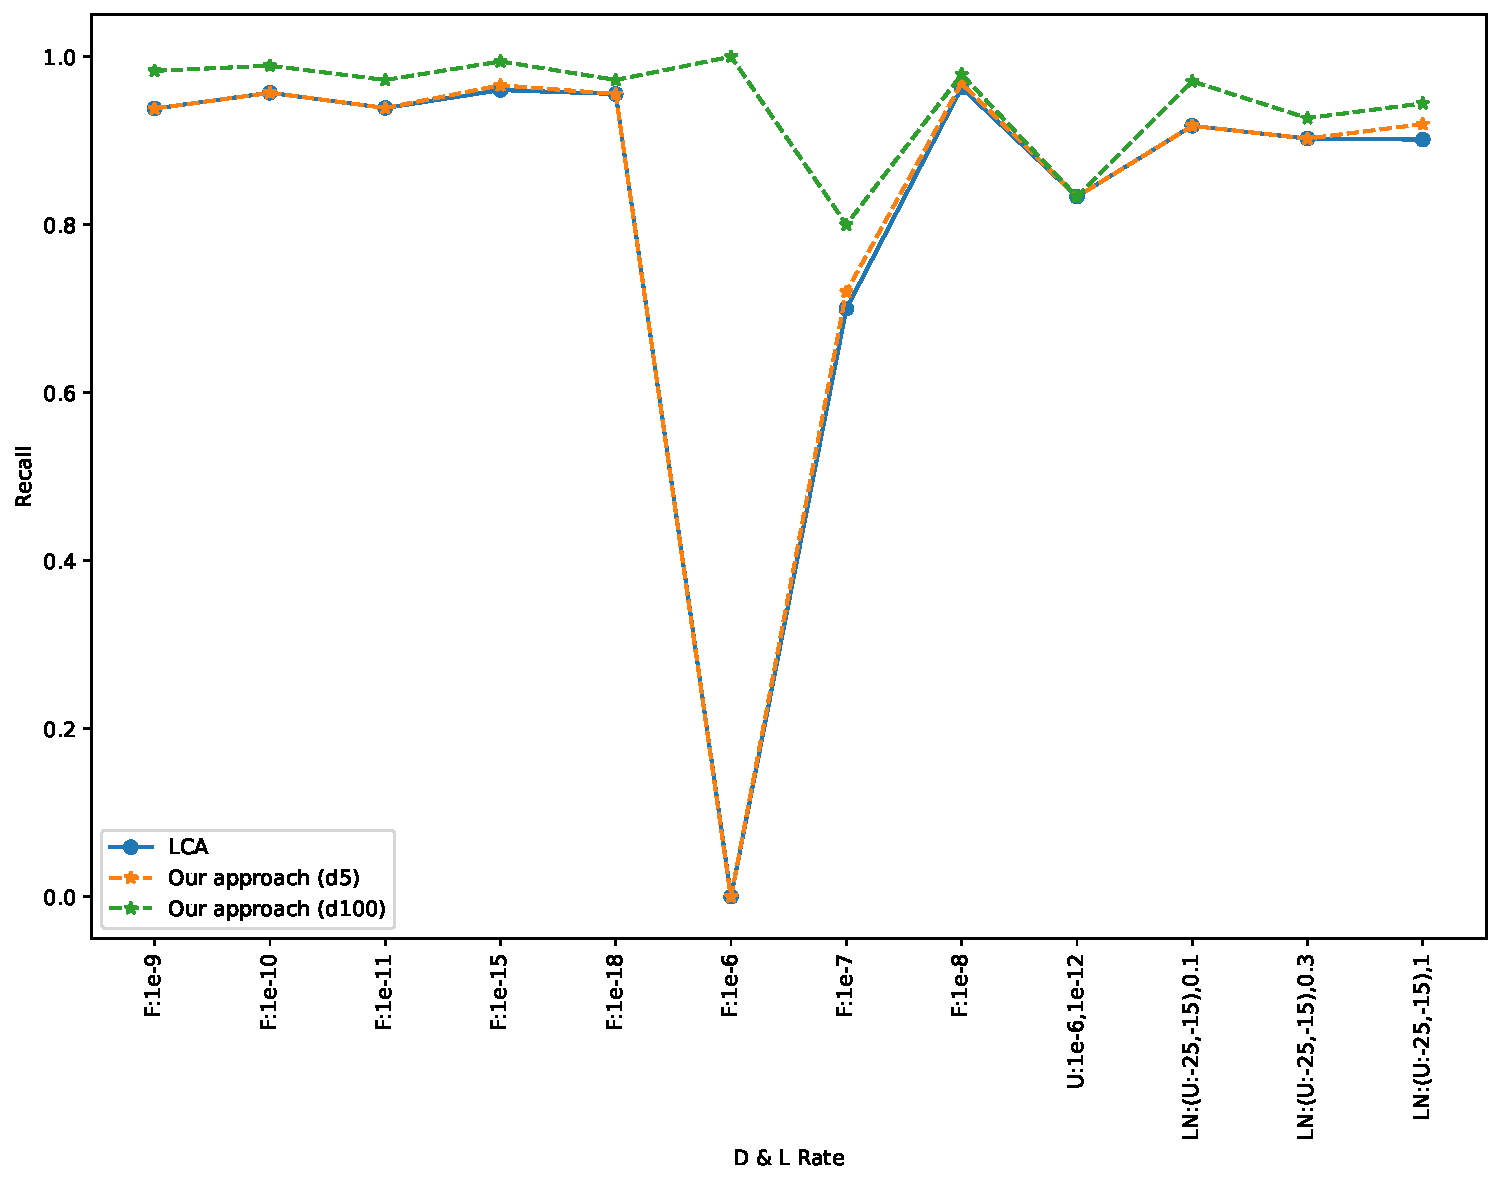
\includegraphics[width=\textwidth]{figs/recall-2W-NNI-K15-WGD-t20-t80-Avg.pdf}
        \caption{Recall of WGDs for simulations with 2 WGD under NNI when k=15, averaged over 100 runs.}
        \label{fig:recall-NNI-k15-2wgd}
    \end{subfigure}
    
    \vspace{1em} % Adds space between the two rows

    % Second row of three subplots
    \begin{subfigure}[b]{0.31\textwidth}
        \centering
        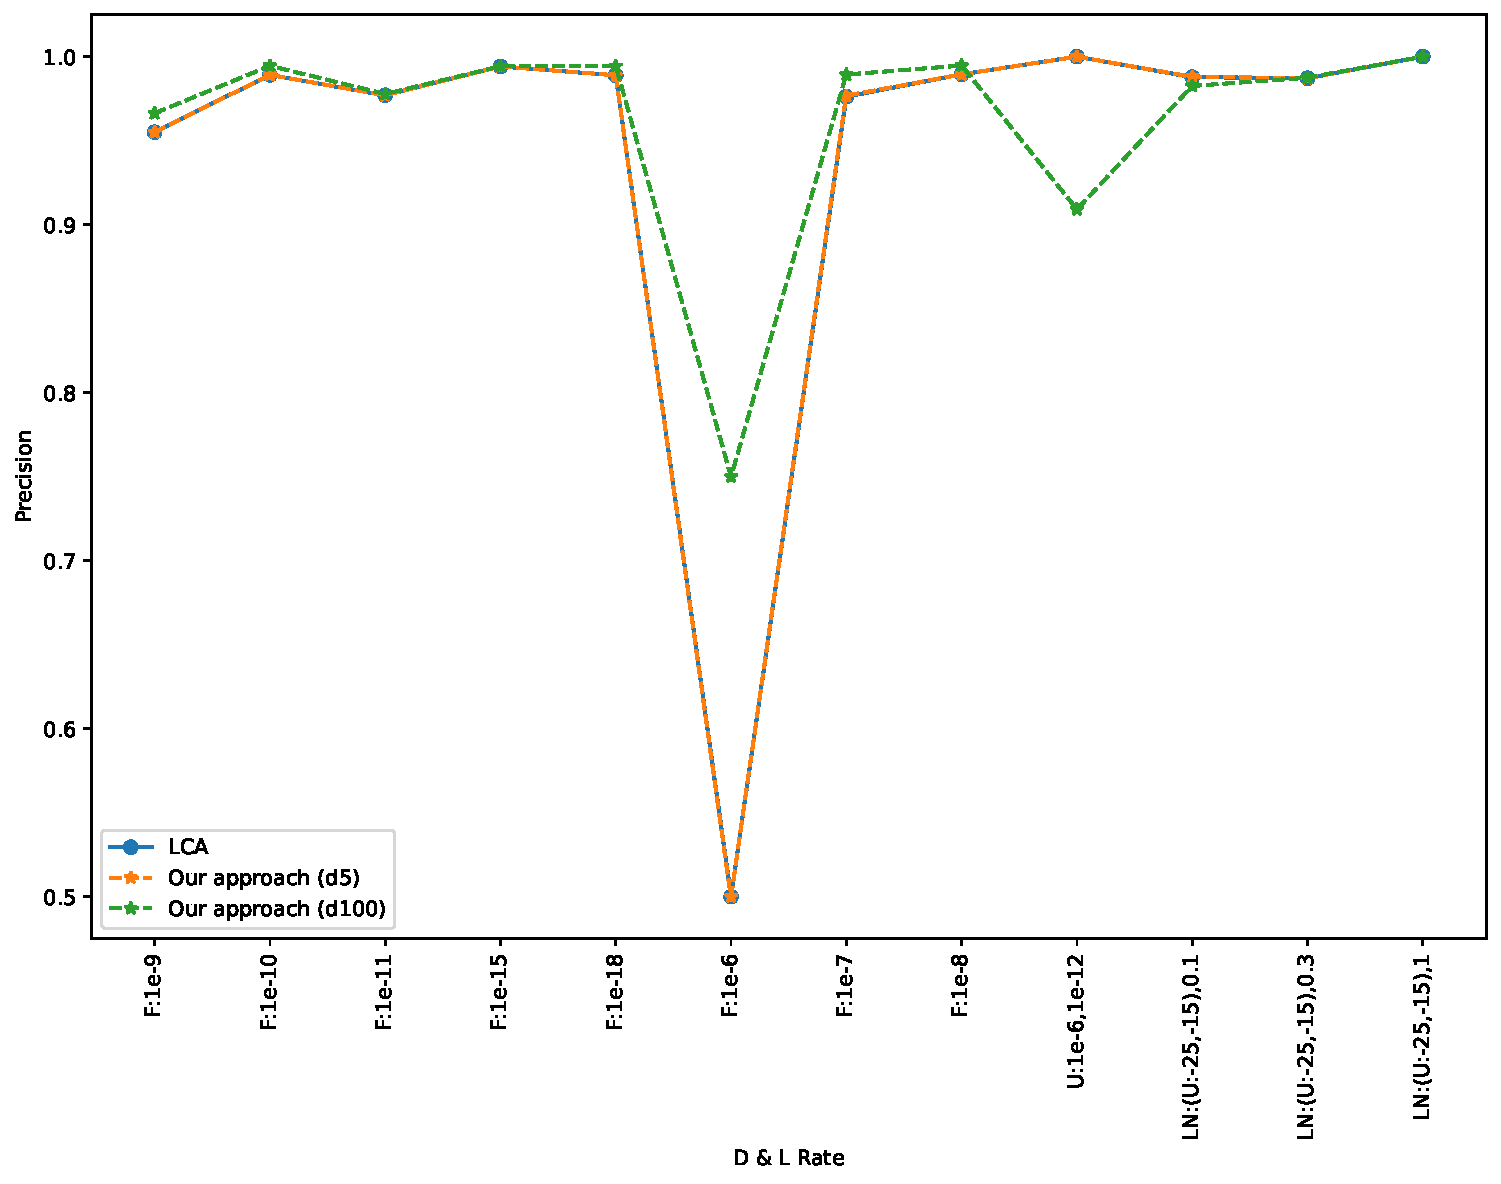
\includegraphics[width=\textwidth]{figs/precision-2W-NNI-K1-WGD-t20-t80-Avg.pdf}
        \caption{Precision of WGDs for simulations with 2 WGD under NNI when k=1, averaged over 100 runs.}
        \label{fig:precision-NNI-k1-2wgd}
    \end{subfigure}
    \hfill
    \begin{subfigure}[b]{0.31\textwidth}
        \centering
        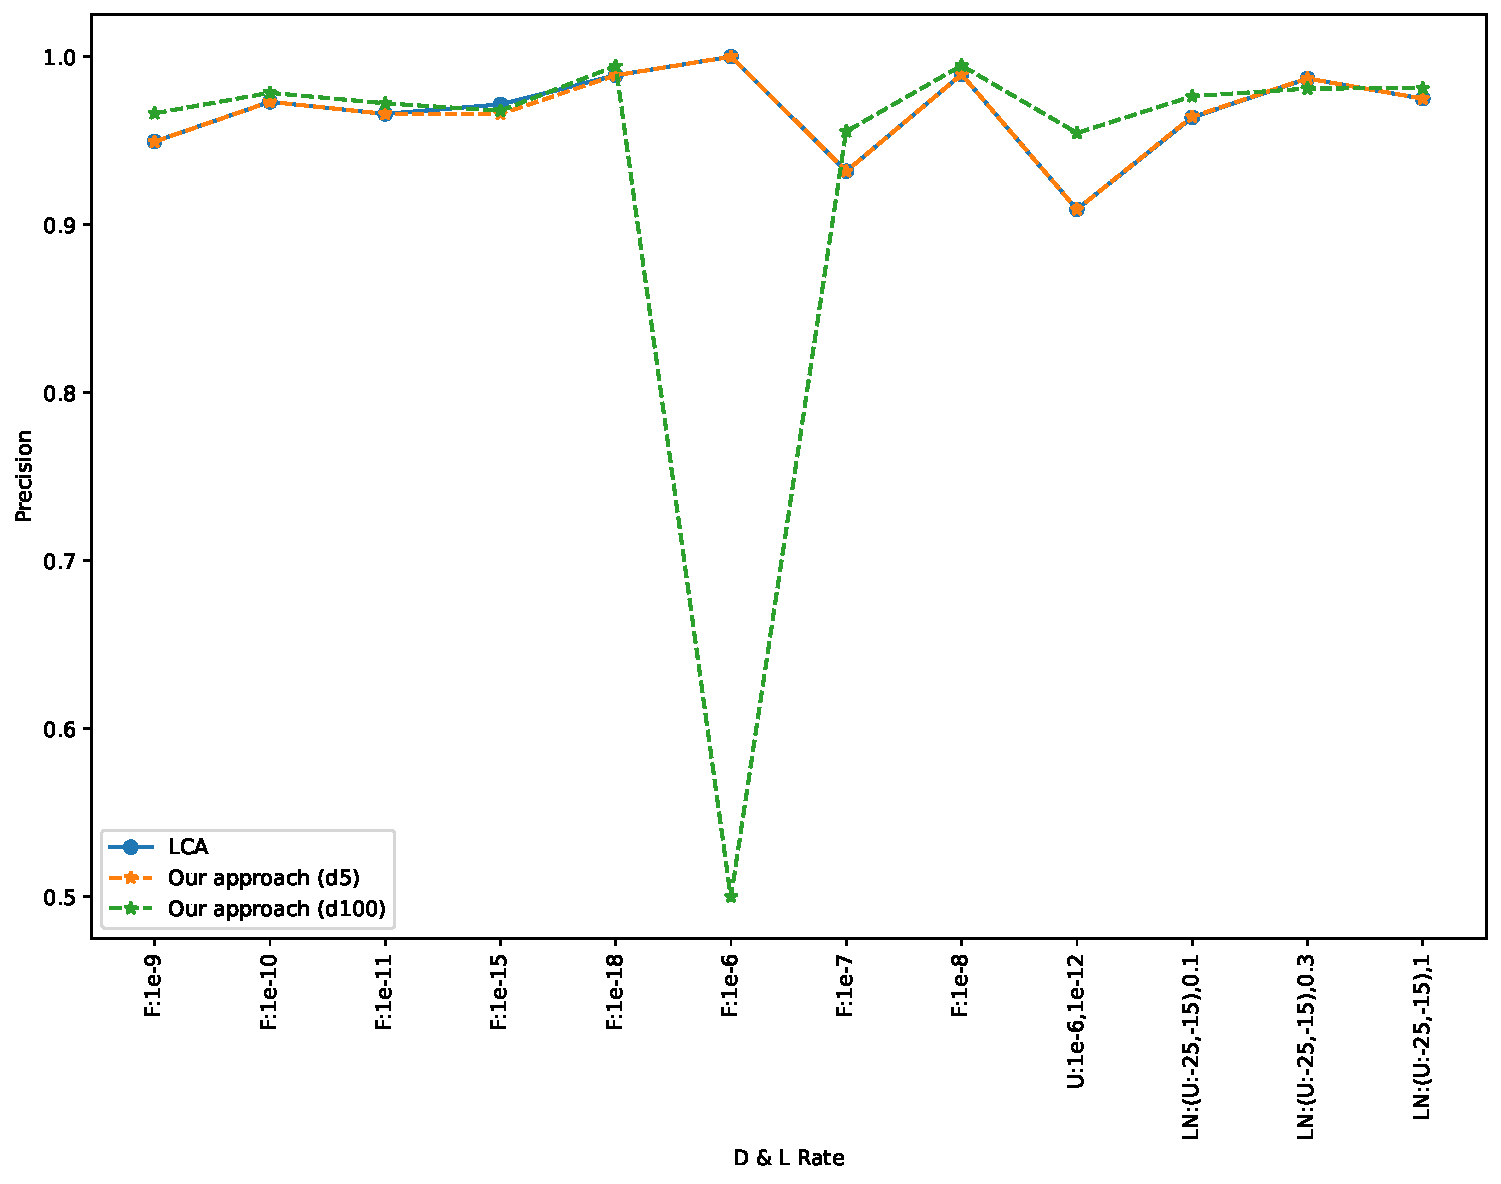
\includegraphics[width=\textwidth]{figs/precision-2W-NNI-K5-WGD-t20-t80-Avg.pdf}
        \caption{Precision of WGDs for simulations with 2 WGD under NNI when k=5, averaged over 100 runs.}
        \label{fig:precision-NNI-k5-2wgd}
    \end{subfigure}
    \hfill
    \begin{subfigure}[b]{0.31\textwidth}
        \centering
        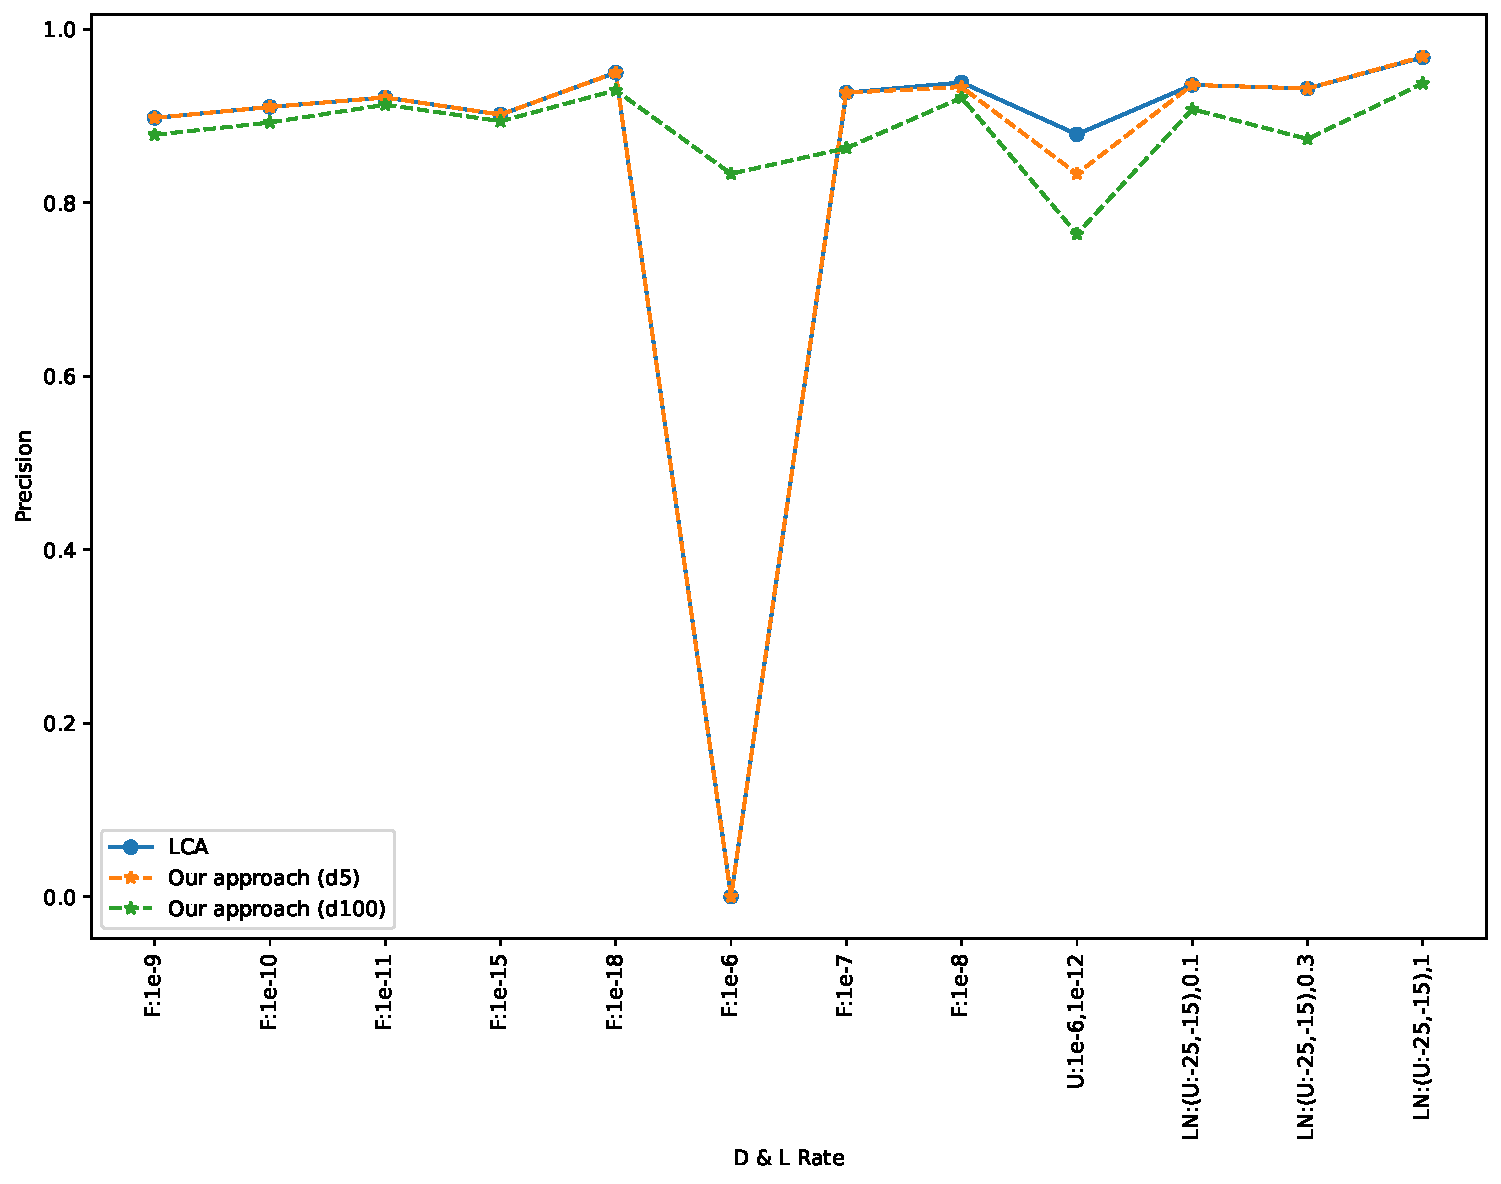
\includegraphics[width=\textwidth]{figs/precision-2W-NNI-K15-WGD-t20-t80-Avg.pdf}
        \caption{Precision of WGDs for simulations with 2 WGD under NNI when k=15, averaged over 100 runs.}
        \label{fig:precision-NNI-k15-2wgd}
    \end{subfigure}
    
    \caption{
        Comparison of Recall and Precision metrics for predicting Whole Genome Duplications (WGDs) in simulations with 2 WGD under Nearest Neighbor Interchanges (NNI) events. The parameter $k$ represents the number of NNIs applied to each gene tree. The simulations span varying duplication and loss rates and are averaged over 100 runs. Subfigures (a), (b), and (c) show Recall metrics for $k=1$, $k=5$, and $k=15$ NNIs, respectively. Subfigures (d), (e), and (f) present the corresponding Precision metrics under the same conditions.
    }
    \label{fig:recall-precision-2wgd-NNI}
\end{figure}

\newpage






\section{Acknowledgments}
This work was supported by French Agence Nationale de la Recherche through the CoCoAlSeq project (ANR-19-CE45-0012). This is the contribution ISEM 2024-XXX of the Institut des Sciences de l’Evolution de Montpellier.


\bibliographystyle{plain}
\bibliography{ref}

\end{document}






































%ARCHIVE OF OLD STUFF




\subsection{Down moves}

\begin{lemma}
    Let $u \in V(G)$ and let $s$ be a descendant of $m(u)$.  Then $\Delta(u, s) = \Delta(u, s, m(u)) + \Delta(u, s, s)$.
\end{lemma}

\begin{proof}
    todo, the idea is that only those can change
\end{proof}


\begin{lemma}
    Let $u \in V(G)$ and let $s$ be a descendant of $m(u)$.  Then:
    \begin{itemize}
        \item 
        if some child $u'$ of $u$ satisfies $m(u') = s$ and $u' \in B[s, H_m(s)]$, then $\Delta(u, s, s) = 1$;

        \item 
        if $u$ is a $dup$ under $m[u \rightarrow s]$ and $H_m(s) = 0$, then $\Delta(u, s, s) = 1$;

        \item 
        otherwise, $\Delta(u, s, s) = 0$.
    \end{itemize}
\end{lemma}

\begin{proof}
    First suppose that $u$ has a child $u'$ with $m(u') = s$ and suppose that there is some $h$ such that $u' \in B[s, h]$.  If a choice for $u'$ arises, assume that $u'$ is chosen so that $h$ is maximum.  
    When we remap $u$ to $s$, then $u$ will be a $dup$ under $m[u \rightarrow s]$ \ml{why?}.  
    This increases the height of the $s$ subtree rooted at $u'$ by $1$.  If $h = H_m(s)$, then $u' \in B[s, H_m(s)]$ and the height of the $s$ forest is increased by $1$, which justifies $\Delta(u, s, s) = 1$.
    If $h \neq H_m(s)$, then the subtree of $F_m(s)$ of maximum height is not rooted at $u'$, and remapping $u$ does not increase the height.  In this situation, we fall into the ``otherwise'' case of the statement (as $H_m(s) \neq 0$ because of $u'$) and correctly put $\Delta(u, s, s) = 0$.

    So let us assume that $u$ has no child $u'$ as described above.
    If $u$ is a $spec$ (in $s$), then $H_m(s)$ is unchanged \ml{[why not related to $p_u$?]}.  If $u$ is a $dup$, then $u$ is the root of a subtree in $s$ of height $1$.  This is an increase in $1$ if and only if $F_m(s)$ had height $0$, as stated.  
\end{proof}




\begin{lemma}
    Let $u \in V(G)$ and let $s$ be a descendant of $m(u)$.  Then:
    \begin{itemize}
        \item 
        if $u$ is a root or $p_u$ is not a $spec$ in $m(s)$ under $m[u \rightarrow s]$, 
        then
        \begin{align*}
        \Delta(u, s, m(u)) = 
            \begin{cases}
                -1 & \mbox{if $D[m(u), H_m(m(u))] = \{u\}$} \\
                0 & \mbox{otherwise}
            \end{cases}
        \end{align*}

        \item 
        if $p_u$ is a $spec$ in $m(s)$ under $m[u \rightarrow s]$, then 
        \begin{align*}
        \Delta(u, s, m(u)) = 
            \begin{cases}
                -2 & \mbox{if $D[m(u), H_m(m(u))] = \{u\}$ and $D[m(u), H_m(m(u)) - 1] = \{p_u\}$} \\
                -1 & \mbox{if $D[m(u), H_m(m(u))] = \{u\}$ and $D[m(u), H_m(m(u)) - 1] \neq \{p_u\}$} \\
                0 & \mbox{otherwise}
            \end{cases}
        \end{align*}
    \end{itemize}
\end{lemma}

\begin{proof}
    
\end{proof}








\section{Multiple gene remappings}

We know that in single-gene remapping, we may have cases where if we remap a gene from species $s_1$ to another species $s_2$, we may only increase the number of losses because there are other genes that are already mapped to the species $s_1$ that keep the same duplication height in $s_1$. So, in this case, we can try to remap all these genes at the same time to other species, then in species $s_1$ we will have reduced duplication height.

For this purpose, we take all the genes (as a set $G_s$) that have the maximum height in species $s$ and map them to another species $s_x$, all formulas in this case are similar to single-gene remapping, but the only difference is that $\Delta(u, s, m(u))$ is $-1$. We calculate the change in duplication height and the  change in the number of losses for each gene in $G_s$.

Finally, to calculate the total change, we need to look at the total change in duplication height and the total change in the number of losses.
The total change in duplication height will be the maximum value among all duplication height changes of all genes in $G_s$, $\Delta(G_s,s_x) = \max_{g \in G_s} (\Delta(G_s, s_x)$.
The total change in the number of losses will be the sum of all the changes in the number of losses for each gene in $G_s$, $\Lambda(G_s, s_x)=\sum_{g \in G_s} \Lambda(g,s_x)$. 





\section{Analyze reconciliation trees}
I've analyzed a simulation with our own simulated gene trees and noted points that prevent the greedy algorithm from acting like true reconciliation. In the \ref{sim} table, you can see the information of these simulated gene trees. As you can see in true reconciliation we only have one duplication whereas in lca and greedy we have 3 duplication heights which is not good so we are looking for the reason.

\begin{table}[hbt!]
\centering
\resizebox{1.05\columnwidth}{!}{%
\begin{tabular}{lll|l|l|l|l|l|l|}
\hline
\multicolumn{1}{|l|}{\textbf{D(lca-simphy)}} & \multicolumn{1}{l|}{\textbf{D(greedy-simphy)}} & \textbf{D(ultragreedy-simphy)} & \textbf{C(simphy)} & \textbf{DH(simphy)} & \textbf{NBL(simphy)} & \textbf{C(lca)}         & \textbf{DH(lca)}         & \textbf{NBL(lca)}         \\ \hline
\multicolumn{1}{|l|}{22}                     & \multicolumn{1}{l|}{22}                        & 22                             & 460                & 1                   & 455                  & 442                     & 3                        & 427                       \\ \hline
\textbf{}                                    & \textbf{}                                      & \textbf{}                      & \textbf{C(greedy)} & \textbf{DH(greedy)} & \textbf{NBL(greedy)} & \textbf{C(ultragreedy)} & \textbf{DH(ultragreedy)} & \textbf{NBL(ultragreedy)} \\ \cline{4-9} 
                                             &                                                &                                & 442                & 3                   & 427                  & 442                     & 3                        & 427                       \\ \cline{4-9} 
\end{tabular}
}
\caption{\label{sim}Info about simulated gene trees.}
\end{table}

First of all, there are cases where lca and greedy do not infer any duplications due to losses, for example in \ref{fig:rec1}, but these cases are not easy to handle.

\begin{figure}[hbt!]
    \centering
    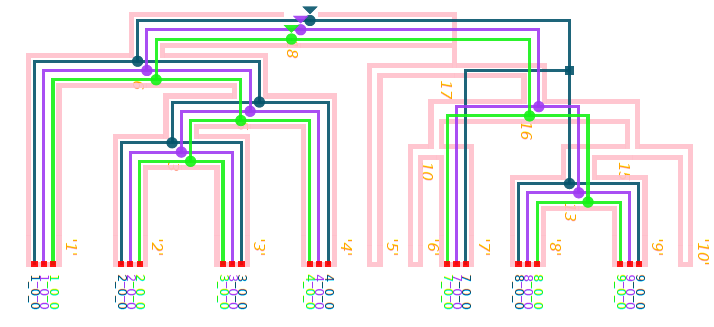
\includegraphics[width=0.85\textwidth]{rec1.PNG}
    \caption{True reconciliation has 1 duplication in species 17, but lca and greedy have no duplication, they just infer it as a speciation in species 16. The outer gene tree is the true reconciliation and the middle tree represents the lca and the inner tree is the greedy reconciliation.}
    \label{fig:rec1}
\end{figure}

Moreover, the above doesn't actually change the height of the duplication because it doesn't infer any duplications, so we'll look at cases that change the duplication.

In figure \ref{fig:rec2} it's an example when lca and greedy infer the duplication in species 16 while the duplication in true reconciliation is in species 17. In this case greedy tries to remap the duplication to species 17 but when it looks at other gene trees, there are other gene trees that have the same situation (lca and greedy have duplication in species 16 instead of 17) so by remapping 16 to 17 duplication height doesn't change, so there is no point for greedy algorithm to remap it (if it remap it just increase number of losses).

\begin{figure}[hbt!]
    \centering
    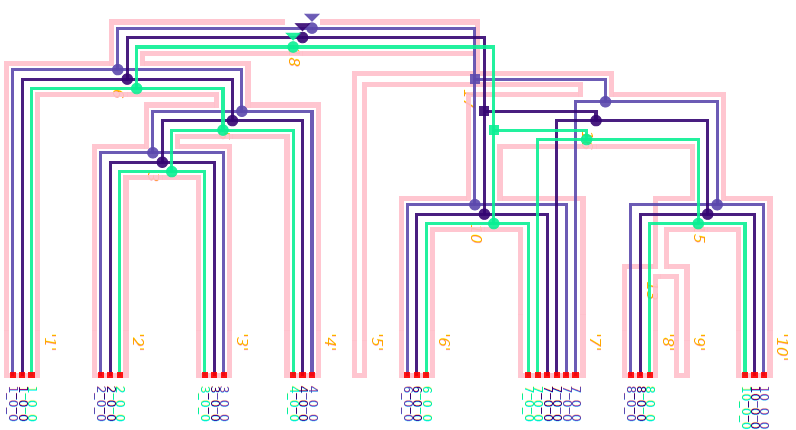
\includegraphics[width=0.85\textwidth]{rec2.PNG}
    \caption{True reconciliation has 1 duplication in species 17, but lca and greedy have one duplication in species 16. The outer gene tree is the true reconciliation and the middle tree represents the lca and the inner tree is the greedy reconciliation.}
    \label{fig:rec2}
\end{figure}

In another example (figure \ref{fig:rec3}) with the same reason as above lca and greedy remap the duplication to species 15 instaed of 17.

\begin{figure}[hbt!]
    \centering
    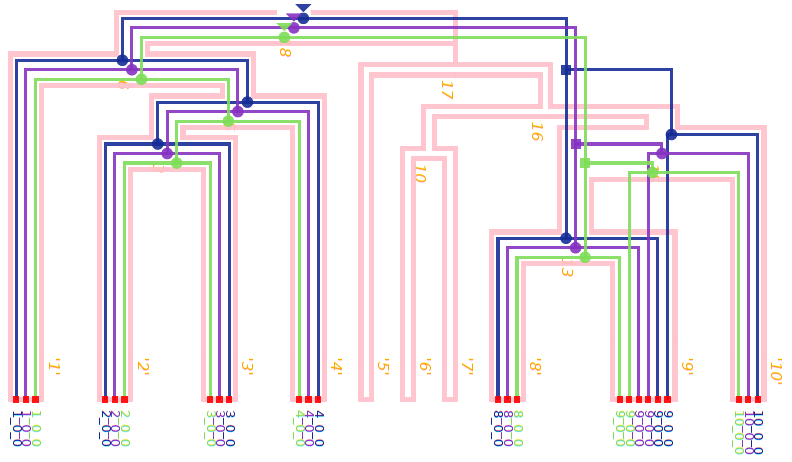
\includegraphics[width=0.85\textwidth]{rec3.PNG}
    \caption{True reconciliation has 1 duplication in species 17, but lca and greedy have one duplication in species 15. The outer gene tree is the true reconciliation and the middle tree represents the lca and the inner tree is the greedy reconciliation.}
    \label{fig:rec3}
\end{figure}

Interestingly, among 100 gene trees, there are only 2 trees where lca infers duplication in species 15 instead of 17. Also, if you remember greedy uses lca mapping as initial step, and greedy progresses the nodes one by one. When it tries to remap one of them, it notices that already in another gene tree we have a duplication in species 15, so there is no point for greedy to remap it to 17.

Solution: Add a feature that can remap some nodes at the same time? Or use another mapping for the initial step?


\section{Gene trees Simulator}
We define a simulator that takes the species tree as input and generates specified numbers of gene trees based on the species tree and some rates. The purpose of this simulation is to simulate segmental duplication.
\subsection{Duplication}
\begin{itemize}
    \item {Branch Length.} the format of species tree is newick and the length of the branch determines the probability of duplication in that branch. For example, if the branch length for node $x$ is 1, we have a repeat at node $x$.

    \item {Rate.} When a node becomes a duplicate, we have two new branches between the duplicate node and the left and right copies that we need to decide on their length (probability of duplication). Rate specifies this length, by dividing the length of the branch of the duplicate node by Rate, we will have the length of the new branches. Just a special case when the rate is 0, the length of the new branch is considered as 0.
\end{itemize}

\subsection{Loss}
After applying duplication to the gene tree, we will apply loss to them. For this purpose we count the number of leaves that are mapped to a specific species. If we called this number $n$ for species $s$, we can have different loss rates for the leaves mapped to $s$.

\begin{itemize}
    \item {Fix Rate.} at this rate, we have a fixed rate ( $(n-1)/n$ ) for all leaves mapped to $s$ , and it will not change even after each leaf is removed.

    \item {Decrease Numerator.} in this rate, we start with the fix rate ( $(n-1)/n$ ) and after removing a leaf, we decrement the numerator by 1 ($(n-1-1)/n$) and so on.

    \item {Decrease Numerator/Denominator} in this rate, we start with the fix rate ( $(n-1)/n$ ) and after removing a leaf, we decrement the numerator and denominator by 1 ($(n-1-1)/(n-1)$) and so on.
\end{itemize}

\subsection{Finalizing gene trees}
In the last step, we need to remove some branches because after duplication actions and losses, some internal nodes may become leaves, which we need to remove. Also, we may have some internal nodes with only one child that we need to remove as well.



\section{Results}
To evaluate our algorithms (both the greedy and stochastic versions), we used SimPhy, a comprehensive simulator of gene family evolution. Initially, we experimented with various rates and distributions for duplication frequency to simulate whole genome duplication (WGD) in SimPhy simulations. However, we found that SimPhy consistently generates random duplications in the simulations and does not specifically simulate WGD. 

\subsection{In-house simulator}
To better evaluate our algorithms, we developed an in-house simulator\footnote{\href{https://github.com/r3zakalhor/Gene-Trees-Simulator-Segmental-duplication-.git}{https://github.com/r3zakalhor/Gene-Trees-Simulator-Segmental-duplication-.git}} capable of simulating WGD and the results were promising. In Figures \ref{fig:in-house-cost} and \ref{fig:in-house-dist}, we show the cost and path distance between the greedy mapping and true mapping, as well as the path distance between the LCA mapping and true mapping for different types of WGD, duplication rates, and loss rates. We explain every parameter in Table \ref{table:in-house-details}.

\begin{table}[hbt!]
\centering
\resizebox{1.05\columnwidth}{!}{%
\begin{tabular}{|c|l|}
\hline
\multicolumn{1}{|l|}{\textbf{WGD type}}  & \textbf{Description}                                                                                          \\ \hline
\textbf{1}                               & one WGD                                                                                                       \\ \hline
\textbf{1+1}                             & two WGD in different subtrees                                                                                 \\ \hline
\textbf{2suc+1}                          & two successive WGD and one WGD in another subtree                                                             \\ \hline
\textbf{3suc+1}                          & three successive WGD and one WGD in another subtree                                                           \\ \hline
\multicolumn{1}{|l|}{\textbf{Dup rate}}  & \textbf{Description}                                                                                          \\ \hline
\textbf{0}                               & descendants of a WGD node have 0 dup rate                                                                     \\ \hline
\textbf{0.5}                             & descendants of a WGD node have 0.5 dup rate                                                                   \\ \hline
\textbf{1/10}                            & descendants of a WGD node have 1/10 dup rate                                                                  \\ \hline
\multicolumn{1}{|l|}{\textbf{Loss rate}} & \textbf{Description}                                                                                          \\ \hline
\textbf{(n-1)/n}                         & fix loss rate where n is the number of copies of a species                                                    \\ \hline
\textbf{(n-i)/n}                         & changeable loss rate where n is the number of copies of a species and i is the number of copies that are lost \\ \hline
\textbf{(n-i-1)/(n-i)}                   & changeable loss rate where n is the number of copies of a species and i is the number of copies that are lost \\ \hline
\end{tabular}
}
\caption{In-house simulator parameters.}
\label{table:in-house-details}
\end{table}

\begin{figure}[hbt!]
    \centering
    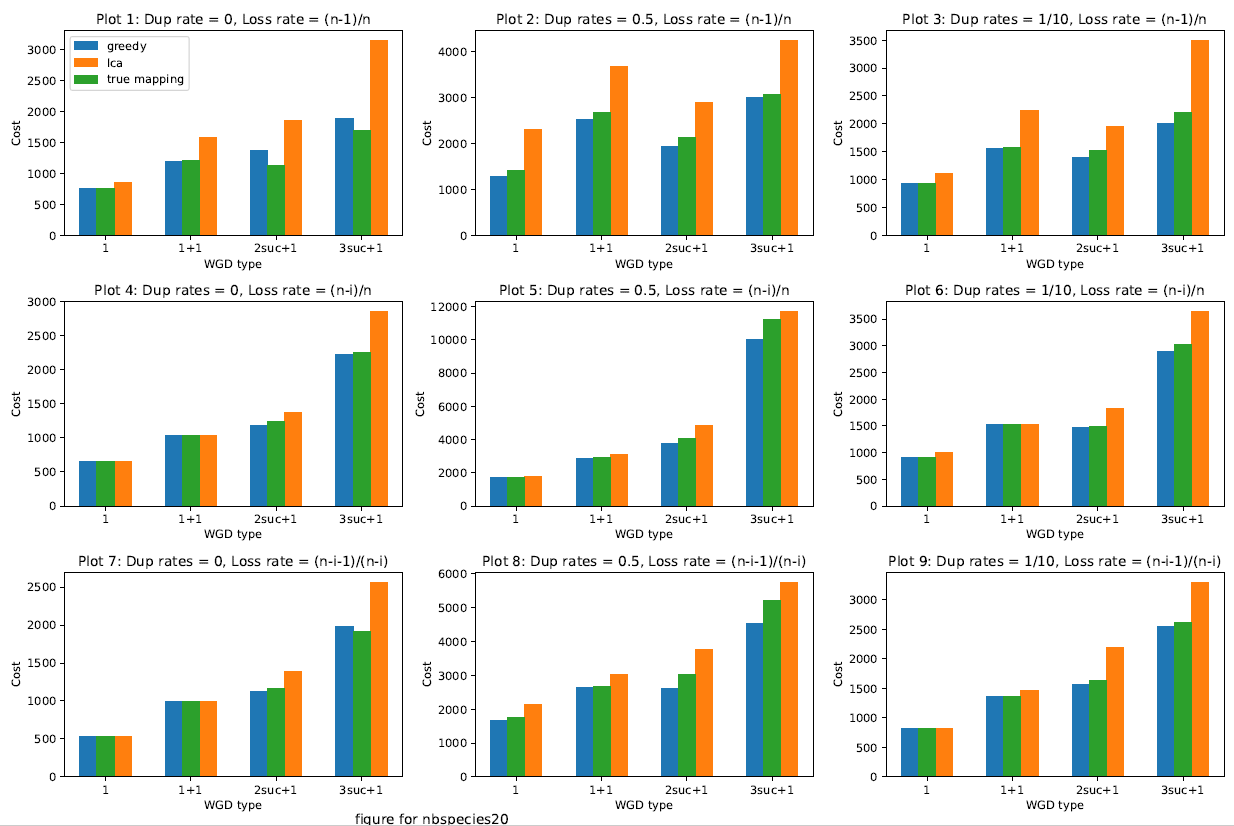
\includegraphics[width=1\textwidth]{in-house-cost-results.PNG}
    \caption{Cost histogram for greedy, lca and true mapping.}
    \label{fig:in-house-cost}
\end{figure}

\begin{figure}[hbt!]
    \centering
    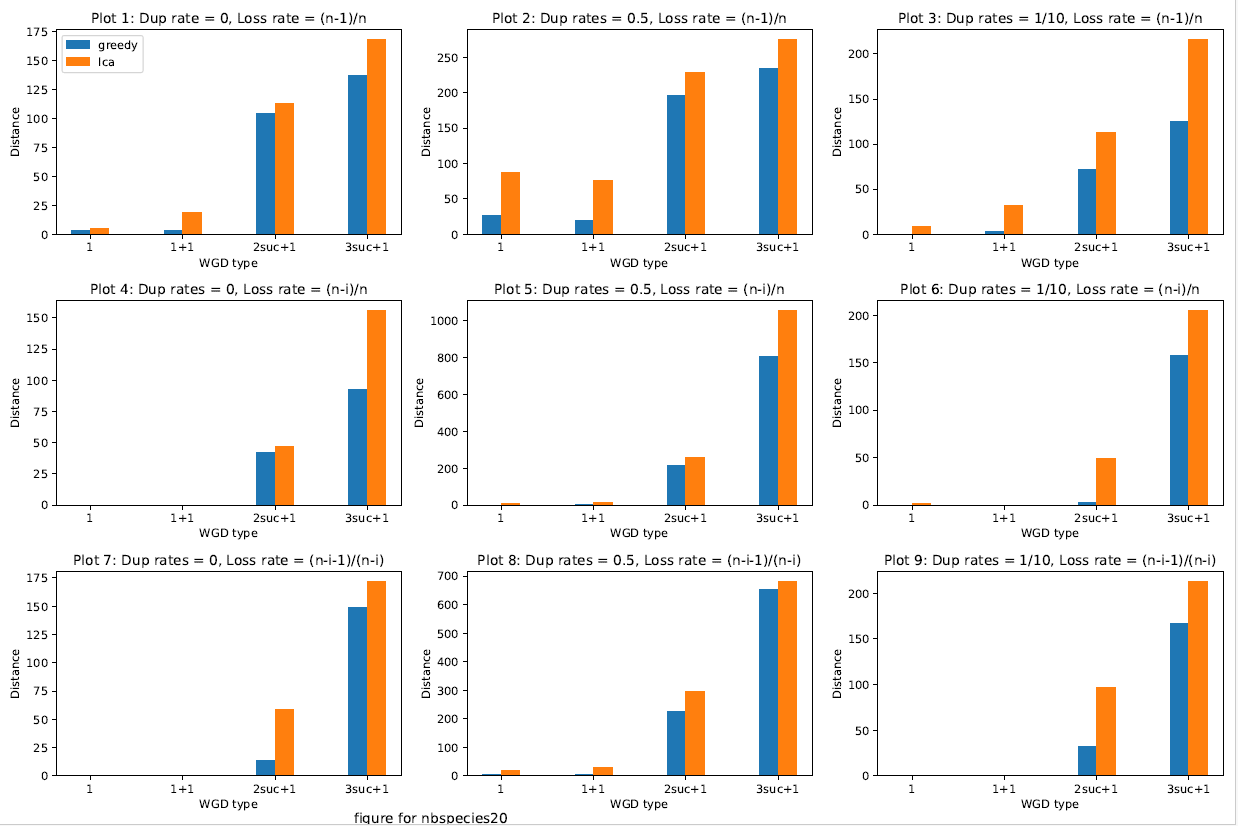
\includegraphics[width=1\textwidth]{in-house-dis-results.PNG}
    \caption{Path-distance histogram for greedy, lca and true mapping.}
    \label{fig:in-house-dist}
\end{figure}